\documentclass[12pt]{article}

\usepackage{hyperref}
\usepackage{amssymb}
\usepackage{amsfonts}
\usepackage{amsmath}
\usepackage{amscd}
\usepackage{amsthm}
\usepackage{amstext}
\usepackage{graphicx}
\usepackage{url}
\usepackage[section]{placeins}
\usepackage{caption}

\usepackage{rotating}
%\usepackage{subfig}
\usepackage{setspace}
\usepackage{lscape}
\usepackage{setspace}
\usepackage{latexsym}       % For funny characters
\usepackage{indentfirst}    % Indents all paragraphs
\usepackage{geometry}       % Increase page margins
\usepackage{epsfig}
\usepackage{yhmath}
\usepackage{footnote}
\usepackage{epic}
\usepackage{wrapfig}
%\usepackage[mdyy]{datetime}
\usepackage{booktabs}
\usepackage{pdflscape}
\usepackage{epstopdf}
\usepackage{bbm}
\usepackage{subcaption}
\usepackage{xcolor}
\usepackage{setspace}
\usepackage{soul}

%%%%%%%%%%%%%%%%%%%%%%%%%%%%%%%%%%%%%%%%%%%%%%%%%%%%%%%%%%%%%%%%%%%%%%%
\usepackage{setspace}
%\usepackage[margin=0.2in]{geometry}
\usepackage{amsmath}
\usepackage{bm}
\usepackage{mathtools}
\usepackage{amssymb}
\usepackage{lscape}
\usepackage{threeparttable}
\usepackage[utf8]{inputenc}
\usepackage{natbib}
\usepackage{lscape}
\usepackage{longtable} 
\usepackage[english]{babel}
\usepackage{graphicx}
\usepackage{color,hyperref}
\usepackage[ruled,linesnumbered]{algorithm2e}
\usepackage{dsfont}
\usepackage{mathrsfs} 
\definecolor{darkblue}{rgb}{0.0,0.0,0.3}
\hypersetup{colorlinks,breaklinks,
	linkcolor=darkblue,urlcolor=darkblue,
	anchorcolor=darkblue,citecolor=darkblue}
\usepackage{epsf}
\usepackage[font=scriptsize]{subcaption}
\captionsetup{compatibility=false}


\onehalfspacing

\setcounter{MaxMatrixCols}{10}
%TCIDATA{OutputFilter=LATEX.DLL}
%TCIDATA{Version=5.50.0.2960}
%TCIDATA{<META NAME="SaveForMode" CONTENT="1">}
%TCIDATA{BibliographyScheme=Manual}
%TCIDATA{LastRevised=Wednesday, April 01, 2015 23:48:48}
%TCIDATA{<META NAME="GraphicsSave" CONTENT="32">}
%TCIDATA{Language=American English}

\geometry {left=1in,right=1in,top=1in,bottom=1in}


%%%%%%%%%%%%%%%%%%%%%%%%%%%%%%%%%%%%%%%%%%%
%%%%%%%%%%%%%%%%%%%%%%%%%%%%%%%%%%%%%%%%%%%


%%%%%%%%%%%%%%%%%%%%%%%%%%%%%%%%%%%%%%%%%%%
%%%%%%%%%%%%%%%%%%%%%%%%%%%%%%%%%%%%%%%%%%%

\begin{document}

\title{Taxing Billionaires:  Estate Taxes and the Geographical Location of the Ultra-Wealthy}
	

\author{Enrico Moretti and Daniel J. Wilson \thanks{Moretti: Department of Economics, University of California, Berkeley (email: moretti@econ.berkeley.edu); Wilson: Economic Research Department, Federal Reserve Bank of San Francisco (email: daniel.wilson@sf.frb.org). We thank the editor, Alan Auerbach, Sebastien Bradley, Jakob Brounstein, Isabel Martinez, Emmanuel Saez, Gabriel Zucman, and seminar participants at the University of California, Berkeley; the Federal Reserve Bank of San Francisco; the University of Nevada; the 2019 NBER Taxation conference; the 2019 Utah Tax Invitational; and the 2019 IIPF annual meetings for useful suggestions. We are grateful to Annemarie Schweinert, Amber Flaharty, and Mary Yilma for excellent research assistance. The views expressed in this paper are solely those of the authors and do not necessarily reflect the views of the Federal Reserve Bank of San Francisco, or the Board of Governors of the Federal Reserve System.}}
\maketitle

%%%%%%%%

\begin{abstract} 
\smaller

We  study the effect of state-level estate taxes on the geographical location of the Forbes 400 richest Americans and its implications for tax policy. We use a change in federal law to identify the tax sensitivity of the ultra-wealthy's locational choices. 
Before 2001, estate tax liabilities for the ultra-wealthy were independent of where they live due to a federal credit against state estate taxes. In 2001, the credit was eliminated and their estate tax liabilities suddenly became highly dependent on where they live.
We find the number of Forbes 400 individuals in estate tax states fell by 35\% after 2001 compared to non-estate tax states. We also find that billionaires' sensitivity to the estate tax increases significantly with age. 
Overall,  billionaires’ geographical location appears to be highly sensitive to  estate taxes. 
When we estimate the effect of billionaire deaths on state tax revenues, we find a sharp increase in  revenues in the three years after a Forbes billionaire's death, totaling \$165 million for the average billionaire. 
In the last part of the paper, we estimate the revenue costs and benefits for each state of having an estate tax.
The benefit is the tax revenue gain when a wealthy resident dies, while the cost is the forgone income tax revenues over the remaining lifetimes of those who relocate. 
Surprisingly, despite the high estimated tax mobility, we find that  the benefit exceeds the cost for the vast majority of states. 
Of the states that currently do not have an estate tax, all but California would experience revenue gains if they were to adopt one. 
\end{abstract}



\thispagestyle{empty}


 
\newpage

\setcounter{page}{1}

\section{Introduction}

The United States exhibits vast geographical differences in the degree to which personal income, corporate income and wealth  are taxed. 
There has been much debate in recent years on the costs and benefits of state and local governments imposing high taxes on their richest residents and most profitable firms, especially in light of the potential for tax flight \citep{moretti/wilson:2017,klevenJEP,zidar}.
But despite the strong interest of policymakers and voters, the effect of state and local taxes on
the geographical location of wealthy individuals and businesses is not fully  understood. Although there have been some important recent advances,  there is still too little empirical work on the effect of taxation on the spatial mobility of individuals, especially among high income individuals. 

In this paper, we contribute to the literature on the  effect of state taxes on
the  locational choices  of wealthy individuals by studying how estate taxes affect the state of residence of the American ultra-rich and the implications for tax policy.
The estate tax is essentially a wealth tax imposed on the very wealthy at the time of death \citep{wo3}.  Specifically, we estimate the effects of state-level estate taxes on the geographical location of the Forbes 400 richest Americans between 1981 and 2017. 
We then use the estimated tax mobility elasticity  to quantify the revenue costs and benefits for each state of having an estate tax. 
We find that billionaires' geographical location is highly sensitive to state estate taxes. Billionaires tend to leave states with an estate tax, especially as they get old.   
But despite the high  tax mobility, we find that  the revenue benefit of an estate tax exceeds the cost for the vast majority of states. 


Estate taxes on the ultra-wealthy have potentially important consequences both for taxpayer families and for state governments. Given the rise of wealth owned by those at the top of the distribution, taxes on large estates have a growing potential to significantly impact states' entire budgets. 
Consider, for example, David Koch who died in August 2019 with an estimated  net worth of \$50.5 billion. He was a resident of New York state, which has an estate tax. Given our estimate  of the effective state estate tax rate (which accounts for typical charitable deductions and sheltering), New York should eventually expect to receive revenues of around  \$4.17 billion.\footnote{In practice, the {\it timing} of estate tax payment depends on marital status and the time of the death of the spouse.} 
For the richest of the Forbes 400, the effect is even larger. As of the time of this writing, Jeff Bezos is the richest person in the U.S., with an estimated net worth of roughly \$200 billion according to Forbes. He resides in Washington state, which has an estate tax. If he died today, his estate could expect to incur a state tax bill of around \$21 billion, almost doubling Washington state's total tax revenues from all sources in a single year. Of course, the typical impact of a Forbes 400 death on state revenues is smaller, though far from trivial, given that the median person in the 2017 Forbes 400 has estimated net worth of ``only" \$3.7 billion. 



%===============================

We begin the empirical analysis by investigating the quality of the Forbes 400 data. 
While prior research has found that individual net worth reported by Forbes is consistent with IRS confidential tax return data \citep{saez2016wealth}, there has been no previous assessment of Forbes  data on state of residence. 
We conduct an audit using published obituaries of deceased Forbes 400 individuals. 
State of death is likely to be highly correlated  with  the  true  state  of  residence,  as  people  are  more  likely  to  die  in  their  true primary residence state than in any other state.\footnote{For estate tax purposes, what matters is the primary domicile state; the physical location of death is irrelevant and thus individuals have no incentive to strategically die in a state other than their residence state for tax purposes.}  We find that the state of residence listed by Forbes matches the state listed in obituaries in 90\% of cases. 

Furthermore, for each  billionaire death, we estimate the effect on  estate tax revenues of the state that Forbes identifies as the one of residence. We find a sharp and economically large increase in estate tax revenues in the three years after a Forbes billionaire's death. We estimate that, on average, a Forbes billionaire's death results in an increase in state estate revenues of \$165 million. 
Our estimate implies an effective tax rate of 8.25\% after allowing for charitable and spousal deductions, and tax avoidance---a rate that is a little over half of the statutory rate. This rate is consistent with IRS estimates of federal estate tax liability for this group of taxpayers. 

% =================================

Having validated the Forbes data, we turn to the core of our empirical analysis, namely  the sensitivity of the ultra-wealthy's locational choice to estate taxes. 
We exploit the sudden change  created by the 2001 Economic Growth and Tax Relief Reconciliation Act (EGTRRA) federal tax reform. 
Before 2001, some states had an estate tax and others didn't. However, there was also a federal credit against state  estate taxes. For the ultra-wealthy, the credit amounted to a full offset. In practice, this meant that 
the estate tax liability for the ultra-wealthy was independent of their state of residence.
%\footnote{As explained  below,  the rate schedule of the credit was such that for the ultra-wealthy (but not for those further down the wealth distribution) the credit fully offset their state estate tax liability. Put differently,  state estate taxes in practice did \textit{not} exceed the credit for, and only for, the ultra-wealthy because every state's top marginal tax rate equaled the top marginal credit rate. In addition, all states had a separate so-called ``pick-up'' tax that was structured to exactly equal the federal credit.} 
The EGTRRA eliminated the credit. The estate tax liability for the ultra-wealthy suddenly became highly dependent on  state of residence.

We first use a double-difference estimator to estimate the differential effect of having an estate tax before versus after 2001 on the number of Forbes 400 individuals in a state. 
We find that before 2001, there is a slight {\it positive} correlation between estate tax status and the number of Forbes 400 individuals in the state, after conditioning on state fixed effects. After 2001, the opposite becomes true: the number of Forbes 400 individuals in estate tax states becomes significantly lower. On average, estate tax states lose 2.35 Forbes 400 individuals relative to non-estate tax states. The implied semi-elasticity is -0.33. Instrumenting contemporaneous estate tax status with estate tax status as of 2001 yields very similar results, confirming that the OLS result is not due to endogenous estate tax adoption or repeal after the 2001 reform.    

We then turn to  a triple-difference estimator based on the notion that a billionaire's sensitivity to the estate tax should increase as they age. In terms of identification, the triple-differenced models allow us to account for any correlation between changes in the unobserved determinants of Forbes' 400 geographical locations and changes in estate tax status after 2001. We find that the number of older Forbes billionaires in estate tax states drops after 2001 relative to the number of younger Forbes billionaires. The elasticity of location  with respect to estate taxes for older billionaires is significantly higher than the elasticity for the younger billionaires.\footnote{This is consistent with \cite{wo}, who finds that the onset of a terminal illness leads to a large reduction in the value of estates reported on tax returns and that this reduction reflects  “deathbed” estate planning. He interprets this as evidence that wealthy individuals care about disposition of their estates, but that this preference is dominated by the desire to maintain control of their wealth while young and healthy. }



As an alternative way to quantify the effect of estate taxes on Forbes billionaires locational choices,  we study the probability that individuals who are observed residing in  estate tax states before the reform move  to a non-estate tax states after the reform; and, inversely, the probability  that individuals who are observed living in non-estate tax states before the reform move  to an estate tax states afterwards. 
Among billionaires observed in 2001, we find a high probability of moving  from estate tax states to non-estate tax states after 2001 and a low probability moving  from non-estate tax states to estate tax states.  By year 2010---namely 9 years after the reform---21.4\% of individuals who originally were in a estate tax state have moved to a non-estate tax state; while only 1.2\% of individuals who originally were in a non-estate tax state have moved to an estate tax state.
The difference is significantly more pronounced for individuals 65 or older, consistent with the triple-difference models. 



Overall, we conclude that billionaires' geographical location is highly sensitive to state estate taxes. The 2001 federal tax reform introduced large differences in billionaires' estate tax burdens among states where there had been none. These ultra-wealthy individuals appear to have responded by leaving states with estate taxes in favor of states without estate taxes.
One implication of this tax-induced mobility is a large reduction in the aggregate tax base subject to subnational estate taxation. We estimate that tax-induced mobility resulted in 23.6 fewer Forbes 400 billionaires and \$80.7 billion less in Forbes 400 wealth exposed to state estate taxes.

In the final part of the paper, we study the implications of our estimates for state tax policy. 
States face a trade-off in terms of tax revenues. On the one hand, adoption of an estate tax on billionaires implies a one-time estate tax revenue gain upon the death of a billionaire in the state. On the other hand, our estimates indicate that the adoption of an estate tax lowers the number of billionaires residing in the state. In terms of state tax revenue, the main cost is the forgone income tax revenues over the remaining lifetime of each billionaire who leaves the state due to the estate tax (as well as any potential new billionaires that might have moved to the state in the absence of an estate tax). The cost of forgone income tax revenues is, of course, higher the higher is the state's top (average) income tax rate. 
We estimate the revenue costs and benefits for each state of having an estate tax, either just on billionaires or the broader population of all wealthy taxpayers.\footnote{This is not the usual Laffer-curve style trade-off, where states with high tax rates are compared to states with low tax rates. There is little empirical variation in estate tax rates---with virtually all states at either zero or 16\%. While states are free to set different rates, in practice they generally have stuck with 16\%, which is a historical carryover from the 16\% maximum rate in the federal credit. Thus, in our calculations we compare tax revenues in the case where a state adopts a 16\% estate tax with  the case where a state does not adopt an estate tax.}  

We quantify costs and benefits of an estate tax on billionaires, using our estimates of the elasticity of mobility with respect to estate taxes and data on expected life expectancies and the number, age and wealth of billionaires in each state. Surprisingly, 
despite the high tax mobility elasticity, we find that for most states the benefit of additional revenues from adopting an estate tax significantly exceeds the cost of forgone income tax revenue due to tax-induced mobility.

The cost-benefit ratio is 0.69 for the average state,  indicating that the the additional revenues from an estate tax exceed the loss of revenues from forgone income taxes by 31\%.  The ratio varies across states as a function of the state income tax rate and, to a lesser extent, the ages of the state's billionaires. In California, the cost-benefit ratio is 1.45, indicating that if California adopted the estate tax on billionaires, the state would lose revenues by a significant margin. (Currently, California does not have an estate tax.) The high cost reflects the very high top tax rate on personal income in California, which implies that each billionaire leaving the state has a high opportunity cost in terms of forgone personal income tax revenue.
By contrast, in Florida or Texas, the cost-benefit ratio is 0 because there is no income tax. The adoption of an estate tax in these states increases tax revenues unambiguously. We estimate that state revenues in Florida and Texas would increase by \$7.67 billion and \$7.06 billion, respectively, if the states adopted an estate tax. Overall, we estimate that 28 of the 29 states that currently do not have an estate tax and have at least one billionaire would experience revenue gains if they adopted an estate tax on billionaires, with California the lone exception. 

We caution that in our cost-benefit analysis, our measure of costs only includes the {\it direct} effects on state revenues of losing resident billionaires, namely the forgone taxable income. It does not include potential {\it indirect} effects on states if billionaire relocation causes relocation of firms and investments as well as a reduction of donations to local charities. A comprehensive analysis of these indirect effects is beyond the scope of this paper.\footnote{There could also be an additional effect on those who do not leave the state, in the form of increased tax avoidance and reduced saving (beyond what has already occurred in response to the nationwide federal estate tax). Increased tax avoidance is already incorporated in our estimates of the effective estate tax rate, but some of the response may show up as reduced capital income.}

Finally, we extend the analysis to consider the costs and benefits of adopting a broader estate tax,
one that applies not only to billionaires, but to all taxpayers with estate values above \$5.5 million for individuals and \$11 million for couples (the current federal  thresholds).  
%For each state, we compute the costs and benefits of an estate tax on this broader group of wealthy taxpayers under alternative assumptions on the elasticity of mobility. 
%Results are similar to the results for billionaires: states that have a cost benefit ratio below  1 for the billionaire estate tax tend to have a cost benefit ratio below 1 for the broader estate tax.
We find that that the policy implications for states that we draw based on a billionaire estate tax generally extend to a broad estate tax: for most states, the  benefits of adopting an estate tax exceed the costs, whether the tax is imposed on the ultra-wealthy or the merely wealthy.  
%For the latter group, we can't be certain of the exact benefits and costs, since the true elasticity of mobility with respect to estate taxes is unknown. 

Our paper seeks to advance the literature on the sensitivity of high income individuals locational choices to state and local taxes. 
We focus on wealth, while most of the previous literature has focused on personal income taxes. For example, \cite{moretti/wilson:2017} and \cite{akcigit2016taxation} find evidence that top patenters, which have very high income, are quite sensitive to income taxes in their choice of location. \cite{rau} find similar results for high income taxpayers in California.  On the other hand, \cite{young2016millionaire} and \cite{young2011millionaire} find limited evidence of tax-induced mobility of millionaires. \cite{klevenJEP} have a recent survey of the literature.\footnote{There is also a related literature on taxes and international mobility. \cite{akcigit2016taxation} find modest elasticities of the number of domestic and foreign inventors with respect to the personal income tax rate.  \cite{kleven2013migration} study a specific tax change in Denmark while \cite{kleven2013taxation} focus on European soccer players. Both find substantial tax elasticities.} 
Overall, despite the importance of the question for state and local governments, the exact magnitude of the elasticities of the number of rich taxpayers with respect to specific forms of subnational taxation is still poorly documented.  As a consequence, much of the policy debate and actual tax policy choices are based on policymaker ideological priors, rather than solid empirical facts. 

The literature on the geographic sensitivity of individuals to estate taxes is even more limited. Our paper is the first to study the ultra-rich---an increasingly important part of the potential tax base, due to their escalating wealth---and to focus on the large differences in effective tax rates after the 2001 reform. 
Before us, \cite{bakija/slemrod:2004} studied state estate taxes, but their analysis predated the elimination of the federal credit and focused on taxpayers with wealth far below that of the Forbes 400, finding mixed results on tax-induced mobility.\footnote{Bakija and Slemrod exploited the fact that the combined federal and state estate average tax rates (ATRs) varied across states even prior to 2001 for lower-wealth estate taxpayers due to state differences in exemption levels and marginal rate schedules. The pre-2001 federal credit effectively offset any cross-state ATR differences for estates far above \$10 million.} \cite{brulhart2014alleged} looked at the effect of bequest tax differences across Swiss cantons and, in contrast to our findings, estimate that high-income retirees are relatively inelastic with respect to tax rates, while \cite{brulhart_etal2017} studied differences across Swiss cantons in wealth taxes.\footnote{See \cite{wo3} for a review of the literature on national estate taxes and \cite{gale} for a discussion of the equity and efficiency of national estate taxes. More recently, \cite{jakobsen2018wealth} study the effect of wealth taxation on wealth accumulation using individual level data from Denmark, finding a sizable response for the ultra-wealthy.} 



%%\footnote{On business taxation, \cite{suarez2016benefits}  find moderate effects of state corporate taxes on wages, total employment, and land prices, while \cite{giroud2019state} find an effect of business taxes on the number of establishments and establishment size.}
 








%%%%%%%%%%%%%%%%%%%%%%%%%%%%%%%%%%%%%%%%%%%%%%%%%%%%%%%%%%%%%%
%%%%%%%%%%%%%%%%%%%%%%%%%%%%%%%%%%%%%%%%%%%%%%%%%%%%%%%%%%%%
%
%%%%%%%%%%%%%%%%%%%%%%%%%%%%%%%%%%%%%%%%%%%%%%%%%%%%%%%%%%%%
%%%%%%%%%%%%%%%%%%%%%%%%%%%%%%%%%%%%%%%%%%%%%%%%%%%%%%%%%%%%


\section{Background and Key Facts on State Estate Taxes}

\subsection{History and Structure}
State level estate taxes in the United States date back to the early nineteenth century, pre-dating the 1916 adoption of the federal estate tax. In 1924, a federal estate tax credit was enacted for state estate tax payments, up to a limit. This credit remained in place for the rest of the twentieth century.\footnote{The credit was for ``estate, inheritance, legacy, or succession taxes paid as the result of the decedent's death to any state or the District of Columbia'' (IRS Form i706 (July 1998)).}  The credit rate schedule prevailing from 1954 to 2001 is shown in Appendix Table \ref{tab:fedcreditrates} (based on Table 1 of \cite{bakija/slemrod:2004}). The top marginal credit rate of 16\% applied to all estate values above \$10,040,000. Thus, for estates far above this value -- such as those of the Forbes 400  -- both the marginal and average credit rate was 16\%.


In the period 1982-2001---which is the part of our sample period before the reform---between 10 and 27 states had an estate tax, depending on the year.\footnote{See \cite{conway2004diagnosis} for a analysis of the factors behind estate tax status in this period.} These estate taxes had progressive rate schedules, with a top marginal tax rate at or slightly below 16\%, applying to estate values above a threshold. The threshold varied across states but never exceeded \$10 million (\cite{bakija/slemrod:2004}) -- very far below the wealth of even the poorest member of the Forbes 400. Thus, for very high net worth estates, such as those of the Forbes 400, the state tax liability was fully offset by the federal credit.\footnote{The convergence between the federal estate average credit rate and state estate ATR for the highest value estates dates back to at least 1935 (\cite{cooper2006interstate}).} This was not necessarily the case for lower wealth estates, for which   
the federal credit  could be much lower than  the state tax liability.\footnote{In addition to state taxes, before 2001  all states imposed ``pick-up'' taxes. These taxes were designed to 
take advantage of the existence of the federal credit and were identical for all states, so for our purposes they can be ignored.  
Specifically, they were structured such that any estate eligible for the federal credit would face a state tax exactly equal to their maximum federal credit amount. In effect, the arrangement amounted to a transfer of funds from the federal government to the state government, leaving the estate taxpayers unaffected. Hence, state pick-up taxes effected no variation across states in tax liability for any taxpayer and thus we exclude them from our definition of the ET ``treatment'' variable used in the analyses below. Pick-up taxes became effectively void after the elimination of the federal credit.} 

For our purposes, the key implication is that, prior to 2001, the combined federal and state  tax liability of the ultra-wealthy was independent of their state of residence. Thus, state estate taxes should not have had any influence on the locational decisions of ultra-wealthy households during that period.


This situation changed completely with the 2001 Economic Growth Tax Relief and Reconciliation Act (EGTRRA). The EGTRRA phased out the credit between 2002 and 2004, eliminating it completely after 2004.\footnote{The credit was replaced with a deduction. This replacement effected large cross-state differences in the combined federal and state estate ATRs depending on whether or not each state had an estate tax. The EGTRRA also legislated changes to the federal estate tax over the subsequent decade, gradually increasing the exemption amount, gradually decreasing the maximum estate tax rate, and scheduling a one-year repeal in 2010 (though 2011 legislation retroactively reinstated the estate tax to 2010). The reductions in the federal estate tax rate over time slightly reduced the value of the state estate tax deduction and thus slightly reduced the incentive to relocate out of estate tax states. In Section 5, we show that this additional variation (beyond the cross-state variation in estate tax status) does not play a major role in billionaires' location decisions.} 
For our purposes, the main effect of the reform was that combined federal and state tax liability of the ultra-wealthy became highly dependent on their state of residence. Thus, after the reform, state estate taxes could potentially affect the locational decisions of ultra-wealthy households. 
%The  magnitude of effect is one of the questions that we investigate empirically in this paper.

The estate tax provisions of the 2001 reform were largely unexpected. 
%In our empirical analysis we will investigate empirically the  timing of the estimated effects. 
 Likely due to legislative inertia, most states that had an estate tax prior to 2001 left it in place after 2001 and most states that did not have one continued to not have. Yet, over the years since 2001, a number of the states have repealed their estate taxes, while a handful of other states have adopted new estate taxes (see \cite{michael2018survey}).



\subsection{Estate Tax Planning and Avoidance}
\label{section:EstateTaxAvoidance}

%Estate taxes are likely to be particularly important to the ultra-wealthy. They tax wealth, rather than income or consumption, and as such apply to a much larger base. [I commented out this sentence as it is distracting here]
State estate taxes are primarily owed to a single domicile state, which is the one determined to be the decedent's primary state of residence. Specifically, \textit{intangible} assets -- financial and business assets -- are taxed solely by the primary domicile state (if the state has an estate tax). The tax base for \textit{tangible} property, which is primarily real estate, is apportioned to states according to property value. Tangible property is generally a small share of the net worth of Forbes 400 individuals. \cite{raub2010comparison}'s study of federal estate tax returns of Forbes 400 decedents reported that real estate accounted for less than 10\% of total assets on average, while financial assets accounted for 85\%. (The other 5\% was ``other assets,'' which could be tangible or intangible.)     

States consider a long list of both quantitative and qualitative indicators in order to determine the primary domicile state of a decedent.  According to \cite{bakija/slemrod:2004},  relevant criteria include  ``physical  location in the state for more than six months of the year, how many years the taxpayer had lived in the state, strength of ties to the local community, and where the taxpayer was registered to vote and maintained bank accounts, among many other factors. Disputes sometimes arise over which state can claim the decedent as a resident for state tax purposes. Most states subscribe to an interstate agreement that provides for third-party arbitration in such situations.'' Note that location of death is irrelevant for tax purposes.

In practice, not all estate wealth is taxed (either by federal or state authorities). First, wealth bequeathed to a spouse is deducted from the taxable estate prior to estate taxation, though the spouse will need to pay estate taxes when they die if the wealth is still above the estate tax threshold. Wealth bequeathed to others, including children, is fully subject to the estate tax.  Inter-vivos gifts (in excess of small annual exemptions) are effectively made subject to the estate tax via gift taxes (which are nearly always paired with estates taxes).\footnote{At these levels of wealth, inter vivos giving is not relevant to shielding beyond a small percentage of the estate value.}


Second, charitable bequests are not taxed. IRS Statistics on Income data (SOI 2017) show that estates worth \$20 million or more deducted 24\% of their taxable wealth due to charitable bequests. 
Third, estate taxpayers have some latitude to make valuation discounts on assets that do not have transparent market prices. For example, artwork and the value of privately-held companies can be difficult to appraise. Note that assets in trusts \textit{are} subject to estate taxation as long as the decedent was the trustee (that is, if she controls where assets were invested and who were the beneficiaries).\footnote{\cite{wo2} investigate the temporal pattern of deaths around the time of changes in the estate tax system and uncover some evidence that there is a small timing-of-death elasticity.}

A recent study \citep{raub2010comparison}, utilizing confidential estate tax returns for deceased individuals that had been in the Forbes 400, found that the average ratio of net worth reported on tax returns to that reported by Forbes was 50\%. Accounting for spousal wealth, which is excluded from the estate tax base but is often included in the Forbes wealth estimate, brings the ratio up to 53\%. The authors attributed the remaining gap primarily to valuation discounts.

In our empirical analysis, we estimate the elasticity of the number of billionaires in a state with respect to state estate taxes. The elasticity that we quantify is to be interpreted as inclusive of any sheltering and evasion. This is the reduced-form parameter relevant for policy.  
In the post-EGTRRA world, without the federal credit to offset state estate tax liabilities, an ultra-wealthy individual's potential combined estate tax liability became hugely dependent on their domicile state. For instance, Washington state enacted an estate tax in 2005 with a top rate of 20\%, the highest in the nation. Thus, an individual with a \$1 billion estate could potentially save up to \$200 million in their eventual estate tax liability simply by moving from Washington to Oregon, or any other of the over 30 states without an estate tax. In other words, one's state estate average tax rate (ATR) could vary across states from 0\% to 20\%. Such variation is much greater than the variation in ATRs across states for personal income, sales, or property. Moreover, the estate tax applies not to a single year of income or sales, but to a lifetime of accumulated wealth. Moving to avoid a high personal income tax will lower one's tax liability resulting from the flow of income in that year and each subsequent year they remain in the state. But moving to escape an estate tax effectively avoids estate taxation on a lifetime of income flows net of consumption. Hence, it is quite conceivable that state estate taxes would factor into the tax and estate planning of ultra-wealthy individuals and could potentially affect decisions of the ultra-wealthy regarding where to live, especially as they get older.



\subsection{Which States Have  Estate Taxes}

Data on adoption and repeal dates of state estate taxes came from \cite{michael2018survey}, \cite{walczak2017state}, \cite{conway2004diagnosis} and \cite{bakija/slemrod:2004}, augmented as needed with information from individual state tax departments. 

For the billionaires in the Forbes 400, the primary geographic variation in the combined federal and state estate tax burden after the 2001 EGTRRA elimination of the federal credit is due simply to which states have an estate tax and which do not. The top marginal estate tax rate -- which approximates the average tax rate for the ultra-wealthy -- is nearly uniform across states that have an estate tax. Of the 13 states with an estate tax in 2017, 10 had a top credit rate of exactly 16\%, one (Hawaii) had a top rate 15.7\%, one (Maine) had 12\%, and one (Washington) had 20\%.\footnote{An additional state, Connecticut, had an estate tax of 16\% up until 2010, 12\% from 2010 to 2015, and then instituted a \$20 million maximum estate tax limit in 2016 (equivalent to an estate tax rate of 2\% for an estate worth \$1 billion).} 
%[I commented out the following sentence since we are not including inheritance tax anymore: And among the 5 states with an inheritance tax (instead of an estate tax) in 2018, the top rate on collateral heirs ranged from 15\% to 18\%.]

Given this uniformity in the estate ATR for billionaires across estate tax states, our baseline analysis uses a simple state-by-year indicator variable for whether or not the state has an estate tax in that year, though the results are consistent if we use the estate tax {\it rate} instead (as shown in Section \ref{section:EIeffects}).\footnote{In our baseline analysis we do not include inheritance taxes, which a handful of states have had during our sample period, in this indicator variable because they typically have a zero or very low tax rate on inheritances by lineal heirs (parents, children, grandchildren, etc.). As we show in Section \ref{section:EIeffects}, our results are not sensitive to this choice. As mentioned earlier, we also do not include in the indicator the separate pick-up taxes that all states had prior to 2001.} 
%Recall that these stand-alone estate taxes generally had top marginal rates near but not exceeding 16\% (the maximum federal credit rate) and those rates went into effect on wealth levels far below the minimum wealth of the Forbes 400. Thus, these stand-alone estate taxes would have had negligible influence on the ATR for the ultra-wealthy. Our diff-in-diff research design allows for the possibility that these pre-2001 estate taxes affect the location choices of the Forbes 400 despite the strong hypothesis that it \textit{should} not affect those choices. An alternative design would be to impose this hypothesis, limit the analysis to the post-2001 period, and simply assess whether the Forbes 400 are less likely to live in ET states than non-ET states. The advantages of the diff-in-diff approach are two-fold. First, it allows for the possibility that even those negligible tax liabilities affect the behavior of the Forbes 400 (or affected their locational choice before they reached Forbes-level wealth). Second and more importantly, by allowing for state fixed effects, it controls for state amenities  that could be correlated with estate taxes.
The maps in Figure \ref{fig:EImaps} show which states had a estate tax, and for how many years, both before and after the elimination of the federal credit. Though there is within-state variation over time, it is clear that most states with an estate tax after 2001 already had an estate tax prior to then, likely due to historical precedence and policy inertia.

It's important to note that states with estate taxes are not necessarily the states with high personal income taxes. California, for example, has the highest top personal income tax rate in the nation, but has no estate tax, while Washington state has no income tax but the highest estate tax rate in the nation. 

Appendix Figure \ref{fig:PIT_dist} shows the distribution of top personal income tax rates (from \cite{moretti/wilson:2017}) across all states by state estate tax status in 2001 (top) and in 2017 (bottom). In both years, estate tax states and non-estate tax states have wide dispersion in top income tax rates, indicating a less than perfect correlation between estate status and income tax rates on high income taxpayers. The vertical red line indicates the average. On average, the mean income tax rate of estate tax states in 2001 is slightly above that of non-estate tax states. However, the mean rates in the two groups of states are almost unchanged between 2001 and 2017. Overall, Figure \ref{fig:PIT_dist} suggests that while there is some correlation between estate status and personal income tax rates, it is not very strong and, more importantly, it has not changed much over the years. 

To see more formally if adoption of estate taxes is correlated with changes in other types of state taxation or the state business cycle, we use a linear probability model to estimate  how the probability that a state has an estate tax relates to other major tax policies and state economic conditions. Specifically, using our full 1982-2017 state panel data set, we estimate a linear probability model of the estate tax indicator on the personal income tax rate, the corporate income tax rate, and real GDP growth, allowing each coefficient to differ pre- and post-2001.\footnote{State GDP data come from \cite{stateGDP}.} The results are provided in Appendix Table \ref{tab:ETadopt}. The coefficients are statistically insignificant in all cases. Controlling for state and year effects yields similar results. We conclude that estate taxes are not systematically correlated with other taxes and the state business cycle -- both in levels and in changes over time. We also show in Section \ref{section:EIeffects} that the results are robust to conditioning on the PIT rate.  


%%%%%%%%%%%%%%%%%%%%%%%%%%%%%%%%%%%%%%%%%%%%%%%%%%%%%%%%%%%%

\section{Data and Facts About the Location of Forbes 400 Billionaires}

\subsection{Data}


Forbes magazine has published a list of the 400 wealthiest Americans every year since 1982.  Forbes defines Americans as ``U.S. citizens who own assets in the U.S.''.  They construct these lists as follows:  Forbes reporters begin with a larger list of potential candidates. They first interview individuals with potential knowledge of the person's assets, such as attorneys and employees, as well as the candidates themselves whenever possible.
They then research asset values using SEC documents, court records, probate records and news articles. Assets include ``stakes in public and private companies, real estate, art, yachts, planes, ranches, vineyards, jewelry, car collections and more.'' Forbes also attempts to estimate and net out individuals' debt, though they admit that debt figures can be difficult to obtain, especially for individuals associated with privately-held businesses.  For more details on their methodology, see: \url{www.forbes.com/forbes-400}.

We collected  the published Forbes 400 tables from 1982 to 2017 (\cite{forbes}). Data for the years 1982 to 1994 were originally in paper format and were digitized by us; the reminder was in electronic format.  
These tables include each individual's name, net worth, age, source of wealth, and residence location.\footnote{The Forbes 400 data we obtained for 2002 did not include state of residence and hence 2002 data are not used in our analyses. Also, data for some years (1995-1998 and 2001) did not include age, though we were able to calculate it using age information for the same individuals from other years.} The listed residence location is typically a single city and state, though there are many instances of multiple listed locations. We record all listed locations, though in our empirical analyses we assume the first listed state is the primary residence. Our results are robust to dropping observations with multiple states of residence. Because the name string for a given individual often has slight variations in the Forbes list from year to year (e.g., William vs. Bill or including vs. omitting a middle initial), we performed extensively cleaning of the name variable in order to track individuals longitudinally.


As has been noted elsewhere (e.g., \cite{saez2016wealth} and \cite{smith2019}), there has been a stark increase over time in the wealth of the super rich in the US in general, and Forbes 400 in particular. Appendix Figure \ref{fig:avg_wealth_tsgraph} plots average wealth over time, in both real and nominal dollars. (Throughout the remainder of the paper, dollars values are in constant 2017 dollars.) 
The Figure shows that in real terms, the wealth of the average Forbes 400 billionaire has increased tenfold since 1982.\footnote{The wealth tax base of the Forbes 400 is a non-trivial share of total wealth in the U.S. \cite{saez2016wealth}  estimate that as of 2013 the Forbes 400 owned about 3\% of total wealth.}

Panel A of Appendix Table \ref{tab:summstats} shows summary statistics. We have 13,432 individual-year observations, covering 1,755 unique individuals. Over the 1982-2017 sample period, the median age of a Forbes billionaire was 65 and their median real wealth (in 2017 dollars) was \$1.6 billion. Mean wealth, however, was much higher, at \$3.02 billion, reflecting the highly skewed wealth distribution among the Forbes 400. For example, Panel B shows selected percentiles of the wealth distribution in 2017. Wealth increases gradually as one goes from the 1st percentile to the 10th, 25th, 50th, and 75th. It more than doubles going from the 75th to the 90th and increases another sixfold from the 90th to the 99th. 
Lastly, in Panel C, we provide summary statistics at the state-year level given that most of our analysis is done at that level. The average state in this period was home to 7.68 Forbes billionaires and statewide wealth of \$22.63 billion. 


\subsection{Location of Forbes 400 Billionaires}

The Forbes 400 live throughout the United States. However, they tend to be concentrated in some states, such as California, Texas, New York, and Florida. The geographic distribution is not fixed over time. 
Figure \ref{fig:Stockmaps} shows a map of the number of Forbes billionaires in 1982 and 2017. 

Table \ref{tab2} shows in more detail the number of Forbes billionaires by state in 2017 (column 2), their mean wealth in 2017 (column 3), the change in the number between 1982 and 2017 (column 3), the change between 1982 and 2000 (column 4), and the change between 2000 and 2017 (column 5). The maps and the table point to some significant shifts in the population of Forbes billionaires. Between 1982 and 2017, California has become home to an increasing share of the Forbes 400 while Texas has comprised a smaller share. By 2017, California had added 37 Forbes billionaires on net, while Texas had lost 30. This shift likely reflects the shift in wealth generated from the technology sector relative to the oil industry boom of the early 1980's. Within California, the San Francisco MSA has gained 37 Forbes billionaires, confirming the role that new wealth generated in the high tech sector plays, while Los Angeles added only 3. A relative decline in fortunes in the Rust Belt states of Pennsylvania (-12) and Ohio (-7) is apparent. On the other hand, Florida has gained 14 new Forbes billionaires, most of them in Miami, while Wyoming has added 3 in Jackson Hole.  

While the geographical unit of analysis in the paper is the state, in order to provide further geographical detail, Appendix Table \ref{tab3}
reports the 2017 levels in number and mean wealth and the 1982-2017 change in number for the 40 cities (consolidated metro areas (CMAs)) with the largest 2017 number of Forbes billionaires.\footnote{Place names listed in Forbes are mapped to metro areas using crosswalk provided by \cite{maggot}.} The Table indicates that, despite its losses, New York city remains the metro area with the largest number of billionaires in 2017 (80), followed by the San Francisco Bay Area (54), Los Angeles (31), Miami (25), and Dallas (18). Chicago, Houston and Washington, D.C. are the other metro areas with 10 or more Forbes billionaires. 



\subsection{Quality of the Forbes 400 Data}

Forbes data on billionaires net worth and their residence are estimates produced by Forbes' researchers. As such they are likely to contain measurement error. 
Forbes' estimate of the total net worth of individuals in our sample were found by \cite{saez2016wealth} to be consistent with IRS data. Using a capitalization method to estimate wealth from income reported on tax returns they conclude that "the top 400 wealthiest taxpayers based on our capitalized income method have a wealth level comparable to the Forbes 400 in recent years'' (p.573).

Data on location have not been previously validated.
In the next section we provide two pieces of evidence on the quality of the Forbes 400 location data. First, we conduct an audit of obituaries of deceased Forbes 400 individuals, and compare state of residence reported by Forbes with state of death.  We find that the state of residence reported by Forbes generally matches the state of death listed in obituaries.
Second, for each death, we  estimate what happens to estate tax revenues in the state of residence listed in Forbes, in the years following the death. If state of residence reported by Forbes is the same as the true state of residence for tax purposes, we should see an increase in estate tax revenues in the state that Forbes identifies as state of residence.  We find  a significant spike in estate tax revenues in the state that Forbes identified as the state of residence of the deceased. 

Overall,  the amount of measurement error in state of residence reported by Forbes appears to be limited.\footnote{Since our  models relate the number of Forbes billionaires in a state to its estate tax status, random measurement error in the number of billionaires in each state would result in increased standard errors but would not affect the consistency of the point estimates. It is in principle possible that the error in billionaire location in Forbes is not just random noise but is systematically correlated with changes in state estate taxes. This might happen, for example, if following an estate tax adoption by a given state, the existing resident billionaires tend to report to Forbes researchers that they have changed their residence to a non-estate tax state (and the Forbes researchers take them at their word), even if their actual residence has not changed.}
%  [DAN: I REMOVED THIS AS IT WAS TOO DEFENSIVE. Our triple-difference models that compare changes over time in the number of old Forbes billionaires relative to young Forbes billionaires in states that adopt estate taxes and states that do not should be unaffected, as it seems plausible that, even if systematic measurement error of this type exists in our Forbes data, it is not correlated with age.} 
% We note that if this assumption fails, our estimated coefficients can be interpreted as the effect of estate taxes on the location of Forbes billionaires reported for tax purposes (as opposed to the true location of residence). This is akin to estimates in the literature on the effect of taxation of labor supply of self employed when labor supply is measured by reported earnings. In this case, our estimates of the aggregate losses and state loses remain valid.}




%%%%%%%%%%%%%%%%%%%%%%%%%%%%%%%%%%%%%%%%%%%%%%%%%%%%%%%%%%%%%%%%%%%%%%%%


\section{Location of Forbes Billionaires Deaths and Effect on Estate Tax Revenues}
\label{section: deaths_analysis}
Before studying the effect of estate taxes on the location  of Forbes billionaires, in this section we present the findings of an audit using obituaries of deceased Forbes 400 individuals in which we assess how close state of residence reported by Forbes matches the state listed in obituaries.\footnote{see \cite{forbesdeaths}} We then use the same data to quantify the impact of billionaires' deaths on state estate tax revenues. The objectives are to assess the quality of the Forbes data and to empirically estimate what fraction of  wealth at the time of death ends up being actually taxed. We use this effective tax rate in our cost-benefit analyses in Section \ref{section:CB}.

 
\subsection{Validation of Forbes' State of Residence Using Billionaire Deaths}

For estate tax purposes, what matters is the primary domicile state. The physical location of death is irrelevant and thus individuals have no incentive to strategically die in a state other than their residence state for tax purposes.\footnote{As noted above, intangible assets comprise the vast majority of Forbes 400 estates and a decedent's intangible assets are taxable by a {single} domicile state.}
Yet, state of death is likely to be highly correlated with the true state of residence, as people are more likely to die in their true primary residence state than in any other state. 
The correlation between state of death and true residence state need not be one, as individuals in our sample who die may die in a different state due to travels, vacations or other idiosyncratic reasons.

To identify potential deaths, we first identified individuals in our sample who were in the Forbes 400 for at least 4 consecutive years before permanently exiting and that, as of their last observation, were older than 50 and in the top 300 of wealth. The top 300 requirement is useful because some less wealthy individuals may disappear from the sample due to their wealth falling below the top 400 threshold rather than due to death. For this subsample of 152 individuals, we searched online for obituaries. Forbes 400 individuals are often known to the general public, and their obituaries are typically published in major newspapers such as the New York Times and the Los Angeles Times. 128 of these 152 individuals were found to have died; the other 24 had dropped out of the Forbes 400 for other reasons. 

The resulting 128 deceased individuals are listed in Appendix Table \ref{deaths}.\footnote{It is worth noting that 123 out of the 128 (96\%) individuals had at least one child according to the obituaries, underscoring the likelihood of strong bequest motives for the Forbes 400 population.} From the obituaries, we recorded both the state in which the death physically occurred as well as the state of primary residence mentioned in the obituary. We find that for 103 of the 128 cases (80\%) the state where death physically occurred was the same as the primary residence state listed in Forbes. Moreover, the mismatches were frequently due to deaths occurring at out-of-state specialized hospitals such as the Mayo Clinic or while on vacation, as indicated in the obituaries and reported in the last column of Appendix Table \ref{deaths}. After accounting for these factors, the state indicated by the obituary was the same as the primary residence state listed in Forbes in 115 deaths, or 90\%.\footnote{Forbes publishes its list in April of each year. If a death occurs between January and April, it is conceivable that Forbes reported state of death is a function of location of death. Our results do not change if we correlate state of death with a one-year lag in Forbes location.}

Overall, it appears that in the vast majority of cases, the primary residence of the individuals in our sample matched that listed by Forbes. We conclude that the state of residence reported by Forbes appears to be generally accurate in identifying the actual state of residence.
We have done a similar analysis comparing the state of residence (as opposed to state of death) reported in the obituaries to the Forbes state of residence. It seems unlikely that newspaper obituaries, when listing one's primary state of residence, would take into account which potential state of residence would imply the lowest estate tax. However, it is possible that  Forbes magazine could influence what gets reported in the obituary, making the two sources of information not completely independent.  With this caveat in mind, we find that the state of primary residence listed in the obituaries matched that listed in Forbes for 107 (84\%) of the 128 deaths. 


\subsection{Effect of Billionaire Deaths on State Estate Tax Revenues} 
 
For each death, we  estimate what happens to estate tax revenues in the state of residence, as listed in Forbes, in the years following the death.\footnote{The data on estate tax revenues comes from the Census Bureau's Annual Survey of State Tax Collections, item T50 (``Death and Gift Taxes'')(\cite{stc}). We deflate to 2017 dollars using the national CPI-U price index (\cite{CPI}).} If Forbes location is accurate, and Forbes 400 billionaires pay  estate taxes, we should see an increase in estate tax revenues in the state that Forbes identifies as the state of residence. If Forbes location is inaccurate, or Forbes billionaires are able to shelter most of their wealth from estate taxation, we should see limited effect on state estate tax revenues in the state that Forbes identifies as the state of residence. 
If Forbes location is accurate, and Forbes billionaires are able to shelter part of their wealth from estate taxation, the estimated effect will be informative of the effective tax rate for this group.  

Since we are using the time of death to empirically estimate its effect on state estate tax revenues, we focus our analysis on the subset of deaths of unmarried individuals. The reason is that if the deceased is married at the time of death, estate taxes are not due until the time of death of the spouse. To be clear, estate taxes will ultimately need to be paid, irrespective of the marital status of the deceased. However, in the case of married taxpayers, the timing of the payment is a function of the time of death of the spouse, which we don't observe. In our sample of deaths, there are 41 decedents who were unmarried at the time of death.

Figure \ref{fig:case_studies} shows two case studies. The top panel shows estate tax revenues in Arkansas leading up to and after the death of James (``Bud'') L. Walton, co-founder of Walmart along with his brother Sam Walton. Bud Walton died in 1995 and was unmarried at the time. The dashed vertical line in the figure indicates the year of death. As can be clearly seen in the figure, estate tax revenues in Arkansas were generally stable in the years leading up to his death, averaging around \$16 million in inflation-adjusted 2017 dollars between 1982 and 1994. In the year after Walton's death, Arkansas estate tax revenues increased 425\%, from \$34.8 million to \$183.2 million -- an increase of \$148.3 million.\footnote{Arkansas had a ``pick-up'' tax of the type described earlier, not a separate estate tax. The Arkansas pick-up tax expired in 2005 when the federal credit to which it was tied was eliminated. This explains the near-zero estate tax revenues in Arkansas after 2004 shown in the figure.}

Forbes estimated Bud Walton's net worth in 1994 to be \$1 billion, or \$1.65 billion in 2017 dollars. Thus, assuming the \$148 million jump in Arkansas estate tax revenues in 1996 was due solely to Walton's death, this implies that the effective average tax rate on the Walton estate was approximately 9.0\%. 

The fact that this effective ATR is below Arkansas' top statutory tax rate of 16\% is to be expected. Recall from Section \ref{section:EstateTaxAvoidance} that in practice estate taxpayers are able to reduce their effective tax rates by reducing their estate tax base through a combination of charitable bequests, asset valuation discounts, and other tax sheltering measures. In fact, the 9\% effective tax rate on the Walton estate is close to what we would expect from IRS data for this population. Specifically, \cite{raub2010comparison} found that the estate values of Forbes 400 decedents reported on federal estate tax returns is about 50\% of the net worth estimated by Forbes, and IRS Statistics on Income data indicate that for estates with wealth above \$20 million, on average 24\% is deducted for charitable bequests. This implies an effective average tax rate in practice of around 38\% ($50\% \times (1-.24)$) times the statutory tax rate of 16\%, which is 6.1\%.\footnote{According to IRS rules, federal estate taxes are not subtracted from the base before state taxes are calculated.}


The bottom panel of Figure \ref{fig:case_studies} shows estate tax revenues in Oklahoma before and after the 2003 death of Edward Gaylord, a media and entertainment mogul. In the years leading up to and including his death, state estate tax revenues were declining. They jumped in the year after Gaylord's death by approximately \$44 million (in 2017 dollars). The last estimate by Forbes (in 2001) of Gaylord's net worth was \$1.8 billion, equivalent to \$2.49 billion in 2017 dollars. This implies an effective tax rate of just 2\%. The low effective rate can be attributed to some combination of Forbes' estimate being too high, an usually high share of Gaylord's estate going to charity, and/or an usually high degree of tax sheltering.   

Of course, these are just two selected cases. We now turn to our full sample of deaths to estimate the average response of state estate tax revenues to a Forbes 400 death. Figure \ref{fig:event_study} shows the average across all 41 deaths of unmarried individuals in our sample. The figure plots state estate tax revenue from 5 years before a death to 5 years after a death. State revenues are demeaned by national yearly means to account for aggregate year-to-year variation (e.g., due to business cycle and other aggregate movements in asset values).\footnote{In case a state has multiple deaths in different years, we treat them as separate events. There is one case -- Florida in 1995 -- with two deaths in the same state and year. We code this as a single event, though the results are very similar if we code it as two separate events.}

The figures shows that in the five years leading up to a death there is no obvious pre-trend. The horizontal line marks the average revenue between $t-5$ and $t-1$ for a death occurring in year $t$. In the years after a death, we uncover an economically large increase in estate tax revenues. In the year of the death,  state estate tax revenues exceed the pre-death average by around \$45 million (in 2017 dollars).
The peak is in the year following the death, year $t+1$, when state estate tax revenues exceed the pre-death average by around \$65 million. The corresponding estimates for $t+2$ and $t+3$ are \$30 and \$25 million, respectively. 

The average effect does not all occur in a single year (relative to the death year). The timing of estate tax payments can vary from decedent to decedent based on the particular situation. Some payments may occur in the year of the death if the death occurred early in the year and asset valuation was relatively straightforward. In other cases, especially if estate asset valuation is particularly complicated or there are legal disputes, payment may occur a few years after the death. Figure \ref{fig:event_study} depicts the average response over cases.

By summing the difference between the pre-death mean and the tax revenues in the 5 years after death,  we estimate that, on average, a Forbes billionaire death results in an increase in state estate revenues of \$165 million. This estimate, combined with the fact the average net worth of the deceased individuals that we included in Figure \ref{fig:event_study} is \$2.01 billion, implies that this group of individuals paid an effective estate tax rate of 8.25\%. This rate is about half of the typical 16\% statutory average tax rate, suggesting that about half of their Forbes estimated wealth ends up taxed.
This effective rate is close to the 6.1\% back-of-the-envelope effective rate we calculated above based on IRS federal estate tax data \citep{raub2010comparison}.\footnote{In the cost-benefit analysis in Section \ref{section:CB}, we will use the 8.25\% to compute the benefit in terms of tax revenue that states can expect from adoption estate taxes. The qualitative results are similar using the 6.1\% rate instead.}

We draw two main conclusions.  First, following a death of a Forbes billionaire, we see a measurable increase in estate tax revenues in the "right" state, i.e. the state that Forbes identifies as the state of residence. Second, the magnitude of the increase is similar to what we would expect based on IRS data. Having validated the Forbes data, we turn to the core of our empirical analysis, estimating the sensitivity of the ultra-wealthy's locational choice to estate taxes.




%%%%%%%%%%%%%%%%%%%%%%%%%%%%%%%%%%%%%%%%%%%%%%%%%%%%%%%%%%%%%%%%%%%%%%%%%
\section{Effect of Estate Tax on Location of Forbes 400}
\label{section:EIeffects}
We use the elimination of the federal credit for state estate taxes in 2001 for assessing the locational sensitivity of the ultra-rich to estate taxes. Prior to the elimination, all states had essentially the same average estate tax rate for billionaires, combining federal and state liabilities. After the elimination, there was stark geographical variation in estate tax liability depending on whether a state has an estate tax or not.  

Figure \ref{fig:ShareIn2001ET} shows the unconditional share of Forbes 400 billionaires living in states that in year 2001 had an estate tax.   The vertical line marks 2001 -- the year when the tax reform was passed -- and the shaded area marks the phase-out period from 2002-2004. The dashed horizontal lines are the mean before 2001 and after 2001.\footnote{Splitting observations by 2001 ET status, rather than current year ET status, ensures that any post-2001 break in the probability of living in an ET state is not driven by ET adoption or repeal by states.}
The Figure shows that in the years 1977-2001 the ET state share fluctuates between 17.5\% and 19.5\%.  
%If anything, the share appears to be slightly {\it increasing}, although the slope is not significantly different from zero.  
In the years after the end of the phase-in period, the share declines significantly, although not monotonically.  In 1999, 2000 and 2001, the share was 19.5\% and 19.2\% and 19.1\%, respectively. By year 2015, 2016 and 2017, the share has dropped to 12.8\%, 13.5\% and 13.4\%-- a decline of about a third. 

There are no controls in Figure \ref{fig:ShareIn2001ET}. To quantify more systematically the effect of the reform, we start with a difference-in-difference estimator that compares the change in the number of billionaires (or their wealth) prior to the 2001 credit elimination and after the elimination in estate tax states and non-estate tax states.  
%If the ultra-rich locational choices are sensitive to estate taxes, we expect to observe a negative correlation after the elimination.  
Our main empirical specification is based on a triple-difference estimator, where we add a third difference (across age) to the differences across states and before/after 2001. 
Because estate taxes only apply at death and are only based  on the domicile state at that time, billionaires should become more locationally sensitive to estate taxes as they age.  \cite{wo}, for example,  finds evidence that wealthy individuals  care about disposition of their estates significantly more when they are closer to death. In addition, billionaires who work for or run a firm are probably more constrained by firm location than older billionaires who have retired or are not as involved in day-to-day firm activities.   

We also look at the probability that after 2001 individuals switch state of residence away from ET states toward non-ET states. In particular, we estimate the probability that individuals observed in an ET state in 2001 are observed in a non-ET state after the reform; and the probability that individuals observed in a non-ET state in 2001 are observed in an ET state after the reform.

Finally, we quantify the aggregate losses for the state tax base caused by geographical mobility of Forbes billionaires from estate tax states to non estate tax states. 


\subsection{Difference-in-Difference Estimates}

Table \ref{tab:2D} shows the double-difference estimates. The level of observation is a state-year pair, and  the sample includes a balanced sample of  50 states observed for 35 years for a total of 1,750 state-year observations. The dependent variables are the number of Forbes 400 individuals in that state in that year or the total wealth of Forbes 400 individuals in that state in that year.  Because the total across states is approximately a constant 400 every year, the estimates based on number of billionaires would be proportional if we used the share of the Forbes 400 in a state in that year.\footnote{Some years have slightly less than 400 individuals due to missing values for state or age.} 

We regress the number of Forbes 400 individuals in the state-year on only an indicator for whether or not the state has an estate tax and its interaction with an indicator for whether or not the year is post-2001. (Throughout the paper, the phase-out period 2002 to 2004 is included in the estimation sample. Results don't change significantly if it is dropped or if treatment is defined as post-2004.) We include state and year fixed effects in all regressions. The post-2001 indicator itself is absorbed by the year fixed effects. 

In column (1), the coefficient on the estate tax state indicator is positive, indicating that before 2001 the Forbes 400 population was slightly higher in the average ET state than in the average non-ET state.\footnote{Since before 2001 billionaire estate tax liability does not depend on location,  one may expect this coefficient to be zero. 
The fact that it is positive might suggest that states adopting estate taxes before 2001 tend to have amenities that are more attractive for billionaires than states not adopting estate taxes. Put differently, if there is any unobserved heterogeneity across states in amenities, it would seem to be  {\it positively} correlated with estate tax status.} 
By contrast, the coefficient on the interaction term is negative, indicating that the average estate tax state saw a drop of  billionaires after 2001 compared with the average non-estate tax state. 
The coefficient on the interaction term in column (1) is -2.358 (with a standard error of 0.683), suggesting that after 2001 the average estate tax state lost 2.36  billionaires relative to non-estate tax states. 
Since the average number of billionaires in an estate tax state in 2001 was 7.2 (7.01 over the full sample), a drop of 2.36 billionaires represents a 32.8\% decline, as reported at the bottom of the Table.\footnote{Since there is a fixed number of Forbes billionaires, treatment of one state comes at the expense of the control group (the other 49 states). Thus models where the dependent variable is the number of billionaires in a state suffer from a small source of bias. The bias, however, is likely to be negligible since for a treated state there are 49 potential destination states.}

One possible concern is that states that change their estate tax status might also change other forms of taxation. In column (2) we control for the top marginal personal income tax (PIT) rate, by state-year, by including both the rate and its interaction with the post-2001 indicator. For billionaires, the top PIT rate will approximately equal the average tax rate.\footnote{We measure the top PIT rate using an average of the top marginal tax rates for wage and salary income and for long-term capital gains, data for which come from the NBER's Taxsim.} We find that the negative post-2001 effect of the estate tax is robust to controlling for the PIT. This  reflects the limited correlation between estate taxes and PIT taxes across states over time that we discussed in the data section above and lends credibility to the notion that it is changes in estate taxes that affect the changes in the number of billionaires in estate tax states, not other changes in fiscal policies. 

Another potential concern could be the amenity value of non-ET states relative to ET states has increased over time for the very wealthy, leading to an increase over time in the share of the Forbes 400 living in non-ET states for reasons unrelated to the estate tax. If this were true, we would also expect to see an increase over time in the share of all wealthy individuals -- not just those subject to the estate tax -- living in non-ET states. Hence, one way to address this concern is by conditioning on the state's share of the nation's population that are wealthy but unlikely to be subject to the estate tax. To measure this share for each state and year, we use individual-level data from the Current Population Survey Outgoing Rotation Group (CPS-ORG), and calculate the population in each state-year with annual earnings between the 90th and 97th percentiles of the national earning distribution.\footnote{Measuring earnings above the 97th percentile consistently over 1982 to 2017 is not possible due to top-coding. Two other large-scale data sets with individual level income data that is not top-coded do not cover our sample period: the Decennial Census microdata are available only every 10 years and the American Community Survey does not start until 2005.} Column (3) shows the results when we include this ``high earners'' population share variable. The negative post-2001 effect of the estate tax on the Forbes 400 population is little affected, indicating that the effect is not driven by changes in the relative amenity value of non-ET states to the wealthy.

The 2001 EGTRRA federal reform was common to all states and exogenous from the point of view of states. However, in the years following the EGTRRA reform, states were free to adopt new estate taxes or repeal existing ones, and some did. One possible concern is that changes in estate tax status after 2001 may be correlated with unobserved determinants of location choices of billionaires.
In column (4), we instrument estate tax status after 2001 with estate tax status in 2001. The first-stage coefficient is 0.653 (0.097) and the first-stage F statistic is 45.7, indicating a high degree of persistence in estate tax status. The point estimate in column (4) is -3.019 (1.635). One cannot reject the null hypothesis that the IV estimate is equal to the corresponding OLS estimate in column (4), although the IV estimate is not very precise. 
The Hausman test statistic is 1.654 and the p-value is 0.437.\footnote{The reduced form coefficient is -1.457 (0.449) (not reported in the table).}  
The fact that the IV and OLS estimates are not statistically different indicates that the amount of endogenety may be limited. This is consistent with the limited number of states that changed their estate tax legislation after the 2001 federal reform. Recall that only a handful of states that did not have a estate tax in 2001 adopted one later, possibly suggesting a role for legislative inertia. Similarly, only six states that had an estate tax in 2001 repealed it later (as of 2017).

In column (5), the dependent variable is the per capita number of Forbes billionaires in a state.\footnote{State population data come from \cite{population}.} The difference-in-difference coefficient is -0.662 (0.333). 
In column (6), the dependent variables is Forbes reported wealth (in billions of 2017 dollars). 
The coefficient on the interaction term is -16.52 (2.442), suggesting that after 2001 the average estate tax state lost  \$16.5 billion relative to non-estate tax states. The implied elasticity is -39.7\%.\footnote{Note that, as we discussed above, if a decedent owned tangible property (eg, real estate) in multiple states, they actually pay estate taxes to each of those states in proportion to the property value in each. By contrast, intangible property (eg, financial assets) get taxed solely by the primary domicile state. The Forbes wealth estimates are for total wealth of an individual and do not distinguish between tangible and intangible assets. A separate issue is the fact that there is a very strong increase in the wealth of the average Forbes billionaire in our sample period: As shown in Figure \ref{fig:avg_wealth_tsgraph}, after adjusting for inflation, the mean Forbes billionaire is 10 times wealthier in 2017 than in 1982. 
This complicates the calculation of the elasticity, as the baseline average computed in the the years before 2001 is significantly lower than the average in the later years. To compute the elasticity entry in column (6), we conservatively deflate mean real wealth to be constant over the sample period (by dividing pre-2001 wealth by 2017 mean wealth).  The estimated elasticity obtained using non-adjusted wealth (in 2017 dollars) is larger.} 

In columns (7) and (8) we probe the robustness of the estimates. In column (7), the indicator for estate tax status is expanded to include states that have a inheritance tax. In column (8), we drop the years 2002 to 2004, which is the period where the federal credit  for estate taxes was being phased out. Our estimates are robust to dropping these years. 

Next, we consider an alternative specification that exploits not just the variation between states that have or don't an ET, but also the variation in effective ET rates. As mentioned previously, nearly all ET states had the same ET rate of 16\%. However, there remain two sources of variation. First, Maine, Hawaii, and Washington had rates other than 16\% ---namely: 12\%, 15.7\%, and 20\%. Second, while the 2001 EGTRRA phased out the federal credit for state estate tax payments by 2005, it replaced it with a deduction. The value of this deduction for an estate taxpayer in an ET state depends on the federal estate tax rate, which varies over time. This means that the difference in the effective combined federal and state ET rate between ET states and non-ET states will vary over time starting in 2005.\footnote{Consider the effective combined federal and state ET rate after 2004:
$\tau^{combined}_{st} = \tau^{state}_{st} + \tau^{fed}_{t} - \tau^{fed}_{t} \tau^{state}_{st}.$
While $\tau^{fed}_{t}$ is common to all states, and would be absorbed by year fixed effects in a regression with $\tau^{combined}_{st}$ on the right-hand-side, $\tau^{fed}_{t} \tau^{state}_{st}$ is not.}
%Column (9) shows the results of replacing the post-2001 ET-state dummy interaction with a post-2001 ET rate interaction. The point estimate is -24.87 (6.107). If the only variation in rates were 0\% and 16\%, we would expect a coefficient of -14.74, which is the coefficient from column (1) scaled up by 1/0.16. The coefficient is larger, though not statistically significantly different from -14.74.
Replacing the post-2001 ET-state dummy interaction with a post-2001 ET rate interaction, we obtain a point estimate of -24.87 (6.107). If the only variation in rates were 0\% and 16\%, we would expect a coefficient of -14.74, which is the coefficient from column (1) scaled up by 1/0.16. The coefficient is larger, though not statistically significantly different from -14.74.

One concern is that some of the variation over time in the geography of the Forbes 400 individuals reflects changes in the sample.  Every year, there is entry and exit from the sample, as some of less wealthy individuals in the sample are replaced  by  wealthier individuals and some individuals die. 
To assess the sensitivity of our estimates to different definitions of the sample, Panel A in Appendix Table \ref{tab:RestrictedSamples} shows estimates based only on the wealthiest 100 individuals (column 1); 
the wealthiest 200 individuals (column 2); the wealthiest 300 individuals (column 3); and those who are in the sample for at least 10 years. Models in this Panel correspond to the model in column 3 of the previous table. For the wealthiest 300 individuals and those who are in the sample for at least 10 years, the coefficient on the estate tax status interacted with the post-2001 indicator appears similar to that for the full sample, and larger than estimates for the wealthiest 100 and 200 individuals. However, because the baseline pre-reform number of billionaires in the latter two samples are much smaller, the implied elasticities (shown at the bottom of the table) are not very different from those estimated in the full sample. If anything, the elasticity for the top 100 group and for those who are in the sample for at least 10 years appear larger than the corresponding elasticity for the full sample. 

We also explore whether our results are unduly influenced by any single ET state. To do this, we repeat the baseline estimation (column 1) but dropping, one at a time, each ET state from the sample. The results are shown in Panel A of Appendix Figure \ref{newtab33}. We find that the post-2001 ET effect is negative and statistically significant in all cases. In particular, dropping New York state, which is the state with the most Forbes billionaires yields a point estimate that is very similar to the baseline estimate. Dropping Pennsylvania, a state that has lost many billionaires in our time period, yields a point estimate of -1.738 (0.654).

In principle, our results have implications about the elasticity of wealth with respect to a state wealth tax. For example, \cite{poterba2000estate} suggests multiplying the estate tax rate by mortality rate to arrive at a measure of annual burden. Using a mortality rate of 1\% for illustration, a 16\% estate tax change would then be approximately equivalent to a 0.16\% wealth tax change and a wealth tax elasticity of -0.2 equivalent to an estate tax elasticity of -20. In our context, \cite{chetty2016association} estimates a the mortality rate for a 75 year old male in the top 1\% of income is 1.6\%, making a 16\% estate tax equivalent to a wealth tax of 0.26\% and making our estimated estate tax elasticity of -37.3 equivalent to a wealth tax elasticity of -0.60.



\subsection{Triple-Difference Estimates}

If billionaires are sensitive to the estate tax, we expect the probability of a billionaire to live in an estate tax state to be independent of the billionaire's age prior to 2001, but to decrease with age in 2001 onward. 


In Figure \ref{fig:binscatterEI_Age}, each point represents a 1-year age group. Its y-axis value is the fraction of billionaires of that age that live in an estate tax state. This fraction can be interpreted as the probability that a billionaire in the Forbes 400 sample of that age was living in an estate tax state at that time. Hence, this is equivalent to estimating a linear probability model as a function of age. Panel A shows the relationship with age over the pre-reform (2001) sample, while Panel B shows the relationship over the post-2004 sample (after the federal credit was fully phased out). The solid red line in each figure shows the estimated linear relationship between the probability of a billionaire living in an estate tax state and age. 

The figure suggests that the probability of a billionaire to live in an estate tax state increases slightly with billionaire's age prior to credit phase-out, and decreases with age after the credit phase-out. 
%XX ENRICO: I think we should drop the sentence below as it draws attention to the issue of whether "old" should be defined as 70 or 75, which we'd rather not get into.
%The reversal in the age gradient is especially apparent for those above 70 to 75 years old, consistent with the notion that estate tax are most salient for older individuals. 
Appendix Figure \ref{fig:figa1} shows the same exercise using personal income taxes instead of estate taxes. In that case one observes a positive age gradient both in the early period and in the later period, suggesting that the effect uncovered in Figure  \ref{fig:binscatterEI_Age} is specific of estate taxes. 

Figure \ref{fig:AgeGradientByYear} shows the estimated age gradient separately for every year of our sample. The two horizontal dashed lines are the mean pre-reform and mean post-reform age gradients.  
For any given year the confidence interval is fairly large, but it is clear that 
there is a decline in the age gradient after the reform. 
The slope coefficients before 2001 tend to be near zero or slightly positive, while the slope coefficients after 2001 tend to be negative.\footnote{The dip in 2009 appears to be driven by outliers. In particular, there were 3 billionaires moving from estate tax (ET) to non-ET states in that year. We stress that year-to-year variation is volatile due to the relatively small number of individuals (especially movers) in the Forbes 400, which is why we focus not on year-to-year changes but the overall change from pre-reform to post-reform.  Our main estimates are robust to dropping 2009. 
We also note that the small positive age-gradient on average in the pre-reform period could be attributable to a correlation between age and the amenities that happen to be present in non-estate tax states – a correlation that our baseline models address with state fixed effects as well as triple-differencing.} 


Table \ref{tab:3D} shows estimates of triple-differenced models that include the difference between young and old.  
We split the Forbes 400 into young and old, with the latter defined by age greater than or equal to 65, the median age of the Forbes 400 in our sample (as well as the standard retirement age in the U.S.). We regress the number of billionaires by state, year, and age group on indicators for post-2001, ``old,'' estate tax state, the interactions estate tax state X post-2001, estate tax state X old, old X post 2001 and estate tax state X post-2001 X old. The coefficient on that last interaction tests whether older billionaires (relative to younger) are more sensitive to state estate taxes after 2001 than before.

In terms of identification,  the main advantage of triple-differenced models over the difference-in-difference models is that the former allow us to control for the interaction of estate tax (ET) status X post-2001.  Thus, threats to validity stemming from the correlation between unobserved differences across states in the determinants of Forbes' 400 geographical locations and estate status after 2001 are accounted for. For example, if non-estate tax states become more attractive to wealthy taxpayers after 2001 because of policy or non-policy changes correlated with estate tax status---whether personal income taxes, corporate taxes, or any other factor that may affect attractiveness of a state to the ultra-wealthy---the interaction of ET status X post-2001 would absorb such differences.\footnote{Moreover,  the triple difference model allays   concerns about systematic measurement error. Consider the case where  state of residence as reported in Forbes is systematically biased, and more so  after 2001 because Forbes 400 individuals become more likely to mis-report their state of residence to Forbes reporters after 2001 in order to minimize the chance that state tax authorities perceive them as resident of estate tax states. This may introduce bias in the difference in difference models. The triple difference estimates are unbiased if the difference in the measurement error that exists in Forbes estimated location of old billionaires and young billionaires is uncorrelated with changes over time in state estate taxes.}     

We find that older billionaires, compared with younger billionaires, are less likely to live in an estate tax state after 2001.  The coefficient on the triple interaction in column (1) is -0.991 (0.330), indicating that the negative effect of estate taxes after 2001 is greater for older billionaires than younger billionaires. 
This remains true when we condition on PIT (column 2); when we instrument current estate tax status with 2001 status (column 4); when the dependent variable is the per capita number of Forbes billionaires in a state (column 5) or wealth (col 6).     
The estimates are robust to including inheritance taxes (column 7) and to dropping 2002-2004 (column 8). 

We also assess whether the triple interaction effect could be driven by changing amenity values of non-ET states relative to ET states that hold specifically for older wealthy individuals. For example, states like Florida -- which are popular destination states for wealthy retirees and do not have estate taxes -- may have become even more attractive to this subpopulation over time. We address this concern in two ways. First, we note that the negative age gradient shown in Figure \ref{fig:AgeGradientByYear} does not have a gradual negative trend, as one might expect from a gradual shift in amenity values, but rather a sharp break after 2001. Second, we return to the CPS-ORG microdata discussed in the prior subsection and calculate each state's share of the national population (by age group) with annual earnings between the 90th and 97th percentiles. Column (3) shows that the triple-difference results are robust to controlling for this variable, suggesting the results are not driven by changes in the relative amenity value of non-ET states specific to older, wealthy individuals.

As we did for the difference-in-difference models, we replace the ET-state with the ET rate ($\tau^{combined}_{st}$) in the post-2001 interactions to exploit additional variation in the combined federal and state effective estate tax rates. The results are roughly consistent with what one would expect from simply scaling up the estimated effects in column (1) by one over the typical ET rate of 16\%. Column (1) suggests that states with an ET had 2.56 (1.567+0.991) fewer old billionaires after 2001 than before 2001. Scaling that by 1/0.16 yields 15.99, which is similar to the coefficient we obtain of 13.64.

Lastly, we assess the sensitivity of our estimates to different definitions of the sample.  Panel B in Appendix Table \ref{tab:RestrictedSamples} shows estimates based only on the wealthiest 100 individuals (column 1); 
the wealthiest 200 individuals (column 2); the wealthiest 300 individuals (column 3); and those who are in the sample for at least 10 years. Models in this Panel correspond to the model in column 3 of the previous table. Estimates for the wealthiest 300 individuals  and those who are in the sample for at least 10 years appear larger than estimates for the wealthiest 100 and 200 individuals. In terms of elasticities, however, the elasticity for the top 100 group is by far the largest.  The bottom panel in Appendix Figure \ref{newtab33} shows how  the diff-in-diff coefficient changes if we drop one state at the time.  Results are generally robust. 

The level of observation in Table \ref{tab:3D} is a state*year*age-group and the dependent variable is the number of Forbes billionaires. An alternative way to look at the same question is to use individual-level data and estimate how the probability of living in an estate tax state varies with age before versus after 2001. In particular, Table \ref{tab:EI_age} reports estimates from a linear probability model (LPM) where the dependent variable is the probability of living in an estate tax state and the level of observation is an individual-year. Unlike Table \ref{tab:3D}, where we split individuals into just two age groups, here age enters linearly. Driscoll-Kraay standard errors are reported. 

Consistent with Table \ref{tab:3D} and Figure \ref{fig:binscatterEI_Age}, the coefficients from the LPM regressions in column (1) indicate that there was no systematic relationship between estate taxes and age prior to 2001. After 2001, however, the estimates in column (2) reveal a strong negative relationship.\footnote{The slope coefficients from the linear fit regressions shown in Figure \ref{fig:AgeGradientByYear}
are provided in columns (1) and (2) of Table \ref{tab:EI_age}, Panel A.}
Column (3) estimates the difference in the age gradient from before 2001 to after 2001. It is strongly negative and significant. The estimated slope coefficients in column (4), which control for state fixed effects, indicate that over 2001 to 2017, with each additional year of age, the probability of living in an estate tax state falls by -0.23 percentage point.  Given the unconditional probability of a 40-year old billionaire in our sample living in an estate tax state after 2001 is about 22\%, this age gradient implies that, for example, a 50-year old, 70-year old and 90-year billionaire would be expected to have only a 19.4\%, 14.2\% and 9.0\% probability of living in an estate tax state after 2001, respectively. 

In column (5) we add individual fixed effects. 
The estimated slope coefficient is 0.00213, not very different from column (4), although the precision of our estimate drops.\footnote{Of the 13,432 individuals in the sample, 127 switch states over time.
In this specification the coefficient on age turns negative. It is possible that these results reflect a general preference of older individuals for non-ET states that then strengthened after 2001, though we caution that these results are based on the relatively small sample of individuals that switched states at some point.}
Overall,  columns (1) to (5) confirm the findings from the triple-differenced models: after 2001, older billionaires tended to shift from estate tax states and to non-estate tax states more so than younger billionaires.

In the last column, we perform a falsification test by assessing whether there is any similar before- vs. after-2001 difference in age-dependence for the personal income tax. We divide states into a ``high income tax'' group and ``low/zero income tax'' group according to whether or not the state has a top marginal tax rate above 3\%, which is close to the median. We repeat the prior age-dependence regressions but now using the fraction of each age group in a high income tax state as the dependent variable. We find  no difference in age-dependence before versus after 2001. In other words, the negative differential age-dependence after 2001, compared to before 2001, appears to be specific of the estate tax.\footnote{Panel C in Appendix Table \ref{tab:RestrictedSamples} shows estimates based only on the wealthiest 100 individuals (column 1); 
the wealthiest 200 individuals (column 2); the wealthiest 300 individuals (column 3); and those who are in the sample for at least 10 years.}


\subsection{Probability of Moving from an Estate Tax State to a Non-Estate Tax State and Vice-Versa}

An additional way to assess how estate taxes affect Forbes billionaires' locational choices is to look explicitly at individual-level mobility. Here, we focus on the probability that individuals who are observed residing in ET states before the reform physically move  to a non-ET state after the reform; and, inversely, the probability  that individuals who are observed living in non-ET states before the reform move to an ET state afterwards. 
If Forbes billionaires were indeed induced to move away from ET states  after the 2001 reform, we expect to observe  a high probability of moving  from ET states to non-ET states after 2001 and a low probability of moving from non-ET states to ET states.  We also expect this to be particularly true for older individuals.  

For this analysis, we focus on the set of individuals in the Forbes 400 in 2001 that were observed in a different state at some point between 1993 and 2009. For those living in an estate tax (ET) state in 2001, we ask what share of them lived in a non-estate tax (non-ET) state in each year $t$ from 1993 to 2009.\footnote{The share is calculated as the number living in a non-ET state divided by the number of ET state residents in 2001 that are also observed in year $t$. Condition on being observed in year $t$ prevents these moving probabilities from mechanically falling due to sample attrition as $t$ gets further away from 2001.} Similarly, for those living in a non-ET state in 2001, we ask what share of them lived in an ET state in each year from 1993 to 2009. These yearly share are shown in Panel A of Figure \ref{pre}. For each year other than 2001, the blue line is the probability of switching from a ET state to a non-ET state. The red line is the probability of switching from a non-ET state to an ET state.  

Three aspects of the Figure are important for its interpretation.  
First, the focus here is on geographical mobility. If a state switches ET status after 2001, and a billionaire does not move, we are not counting that as a move. 
Second, the sample is unbalanced. Third, recall that data on state of residence is missing in the Forbes 400 for 2002. 

The Figure shows that after 2001, billionaires living in ET states increasingly moved to non ET-states. By contrast, after 2001, billionaires living in non-ET states did not move to ET states in significant numbers. 
Of all of the Forbes billionaires living in ET states in 2001 (and who had not exited the sample by 2003), 6.67\% were living in a non-ET state 2 years later; and of all the Forbes billionaires living in non-ET states in 2001, 0.73\% are observed living in an ET state 2 years later. The difference, 5.94\%, is the net migration  toward non-ET states.  As the Figure shows, this difference tends to grow over time, as individuals have more time to contemplate and initiate moving, although the increase is not monotonic. By year 2010---namely 9 years after the reform---21.43\% of individuals who originally were in a ET state were in a non-ET state; while only 1.2\% of individuals who originally were in a non-ET state were in an ET state.

Panels B and C, respectively, report probability of moving for Forbes billionaires who were 65 and older in 2001 and who were younger than 65. Consistent with the triple-differenced models in table \ref{tab:3D}, these two panels show that most of the switching away from ET to non-ET states is among older individuals. 
Among all the old Forbes billionaires in ET states in 2001, 11.43\% are observed living in a non-ET state 2 years later, while among all of the old Forbes billionaires living in non-ET states in 2001, only 0.76\% are observed in a non-ET state 2 years later. The Figure shows that the difference  grows over time. By contrast, the mobility of
young individuals is much lower, and not systematically correlated with ET status. 
Overall, the findings in Figure \ref{pre} confirm the findings from our difference-in-difference and triple-difference models above.\footnote{Further evidence on the avoidance of the estate tax via relocation for older billionaires relative to younger billionaires comes from examining moving rates over time from the full sample (not just those observed in 2001). We examined 5-year moving rates by year — both for moves from ET states to non-ET states and vice-versa — separately for each age group. For the 65 and over group, we find the average ET-to-non-ET moving rate was about one-third higher after 2001 than it was before 2001, while the average non-ET-to-ET moving rate after 2001 was about half what it was before 2001, consistent with increased avoidance of the estate tax. By contrast, for the under 65 age group, the average ET-to-non-ET moving rate similarly increased by about one-third but the average non-ET-to-ET moving rate more than doubled, inconsistent with avoidance of the estate tax.}


\subsection{Effect of Tax-Induced Mobility on State Aggregate Tax Base}

The 2001 EGTRRA Federal Reform introduced potential tax competition among states where there was none and induced some billionaires to relocate from estate tax states to non-estate tax states.  One first-order effect of such mobility was that it reduced the aggregate tax base for states. Here we use our estimates of the effect of estate taxes on the number of billionaires in a state to quantify the magnitude of the decline in the aggregate tax base caused by mobility. 

Table \ref{tab15}  shows the effect of the tax induced mobility on the total number of Forbes billionaires subject to state estate taxes (row 1) and their aggregate wealth (row 2).  In particular, Column (1) shows the total number of Forbes billionaires subject to state estate taxes in 2001 and their total wealth. 
Column (2) shows the estimated changes due to mobility, obtained by  multiplying the baseline number of Forbes billionaires in 2001 and their 2001 wealth by -0.346 and -0.373, respectively---the estimated elasticities from columns (3) and (7) of Table \ref{tab:2D}. 

Entries indicate that there were 78 Forbes billionaires subject to state estate taxes in 2001, and that tax induced mobility after 2001 resulted in 27 fewer Forbes billionaires subject to state estate taxes. Moreover, \$317.6 billion of Forbes billionaires' wealth was subject to state estate taxes in 2001, and that tax induced mobility resulted in a drop of \$118.5 billion in wealth subject to state estate taxes. This appears to be a large aggregate loss in the estate tax base of states. The way to interpret these numbers is that they represent the long-run effect of mobility stemming from state tax differences on the stock of billionaires and the stock of wealth subject to state estate taxes, rather the annual flow of tax revenues. If we assume an effective estate tax rate of 8.25\% as estimated in Section \ref{section: deaths_analysis} above, the loss of \$80.7 billion implies an aggregate long term loss of tax revenues of \$9.78 billion. Since 11 states had an estate tax in 2001, this amounts to a mean loss per state equal to \$889 million.\footnote{Again, this is not the change in the annual tax revenue flow. Rather it is the overall change in (undiscounted) revenues over all future years from the pool of Forbes 400 billionaires observed in 2001.}    




\section{Costs and Benefits for States of Enacting an Estate Tax}
\label{section:CB}

In section \ref{section:EIeffects}, we found a high elasticity of Forbes billionaires' state of residence with respect to state estate taxes, especially for older individuals. In this section, we study what that estimated elasticity implies for state tax policies. Should estate tax states repeal estate taxes? Should non-estate tax states adopt estate taxes? 

States face a trade-off. On the one hand, adoption of the estate tax implies a one-time estate tax revenue gain for the state when a resident billionaire dies. As discussed in the introduction, the magnitude of this revenue can be substantial, and in some cases it can amount to a significant fraction of a state's overall annual revenue. On the other hand, our estimates indicate that the adoption of an estate tax reduces the number of billionaires residing in the state. In terms of state tax revenue, the main cost is the forgone income tax revenues over the remaining lifetime of each billionaire who leaves the state due to the estate tax, as well as any potential new billionaires that might have moved to the state in the absence of an estate tax. The cost of forgone income tax revenue from a given billionaire is different for different states: it is higher the higher is the state's income tax rate on billionaires, which is approximately equal to the state's top marginal rate.

This trade-off is not the usual Laffer-curve style trade-off that the literature  typically focuses on, where states with high tax rates are compared to states with low tax rates. There is little empirical variation in estate tax rates---with virtually all states at either zero or 16\%. While states are free to set different rates, in practice they generally have stuck with 16\%, which is a historical holdover from the 16\% maximum rate in the federal credit that existed until 2001. Thus, in our calculations we compare tax revenues in the case where a state has a 16\% estate tax with tax revenues in the case where the state has no estate tax at all. This is consistent both with the binary nature of state estate tax choices in practice, and with the variation that is used to identify our empirical estimates of the effect of estate taxes on billionaires' geographical location.  

We seek to compare the magnitude of the costs and the benefits for different states of adopting estate taxes in 2017. We use estimates of the elasticity of location with respect to estate taxes from the previous section. We consider two types of estate tax in turn. First, we provide an analysis of the costs and benefits for states of an estate tax that specifically targets billionaires.
% or more precisely, members of the Forbes 400. 
% I removed this bit because our estimates liekly generalize to all billionaires, not just forbes     
Second, we generalize our findings and provide costs and benefits of an estate tax on the full population of wealthy taxpayers, defined as taxpayers with wealth above the 2017 federal estate tax exemption. This latter analysis is more speculative, as it inevitably depends on an assumption of how the elasticity that we have estimated for the ultra-wealthy maps to the analogous elasticity for the broader population of the ``merely'' wealthy. 


\vspace{0.5cm}

\subsection{An Expression for Costs and Benefits}
To fix ideas, consider the simplest possible case of a representative Forbes billionaire in a representative state. For state $s$ that does not have an estate tax in 2017 and that adopts an estate tax in 2017, we can write the benefit as the present discounted value of additional tax revenues due to the estate tax at the time of death of billionaires who remain in the state after the tax adoption. We can write the cost as the present discounted value of the stream of personal income tax revenues that the state would have received, in absence of the estate tax, from billionaires that were deterred from residing there. The expressions for the benefit and cost are thus as follows:

\begin{equation}
\label{eq1}
     Benefit_s = (\frac{1}{1+r})^{T} \cdot N_{s} \cdot (1 - \eta) \cdot W \cdot \tau_s^{W}  
\end{equation} 

\begin{equation}
\label{eq2}
     Cost_s = \sum_{i=1}^{T}(\frac{1}{1+r})^{i} \cdot N_{s} \cdot \eta \cdot Y \cdot \tau_s^{Y}   
\end{equation}

\noindent where $N_{s}$ is the initial number of billionaires in state $s$ before adoption of an estate tax; $Y$ and $W$ are the taxable income and taxable wealth of the average billionaire;  and $\eta$ is our estimate of the elasticity of the Forbes 400 population in a state with respect to the estate tax indicator. Thus,  $(1 - \eta)N_{s}$ in equation (\ref{eq1}) is the number of billionaires left in the state after adoption and  $\eta N_{s}$ in equation \ref{eq2} is the number of billionaires who leave the state because of adoption.   
$\tau_s^{W}$ and 
$\tau_s^{Y}$ are the state estate tax rate and the personal income tax rate that applies to Forbes billionaires, respectively; $T$ is remaining lifetime for a billionaire or their spouse, whichever is longer (recall that estate taxes are paid when the surviving spouse of a couple dies.);  $r$ is the real discount rate for states.

In practice, the benefits and costs are more complicated because  the effect of estate tax adoption on the number of billionaires was found to vary significantly depending on age. Thus,   we use a more general expression of costs and benefits that allows for the elasticity $\eta$ to vary by age and for states to differ in the the age structure of their billionaire population: 


\begin{equation}
\label{eq3}
     Benefit_s = \sum_{a=0}^{100} \left[ (\frac{1}{1+r})^{T_a} \cdot N_{a,s}W \cdot (1 - \eta_a) \cdot \tau_s^{W}  \right] 
\end{equation}

\begin{equation}
\label{eq4}
     Cost_s = \sum_{a=0}^{100} \left[ \sum_{i=1}^{T_a}(\frac{1}{1+r})^{i} \cdot N_{a,s}Y \cdot \eta_a \cdot \tau_s^{Y}  \right] 
\end{equation}

\noindent where $a$ indexes age;  $\eta_a$ is the estimated elasticity at age $a$;  
$N_{a,s}$ is the initial number of billionaires of age $a$ in the state in the before adoption of the estate tax;   and   $T_a$  is remaining life expectancy of a billionaire at age $a$ or his spouse, whichever is longer.

We use our estimates from the previous section to set ${\eta_a}$. 
In particular, based on Table \ref{tab:EI_age}, column 3, we set ${\eta_a} = 0.002 - 0.00332*a $, where 0.002 is the estimated intercept and $-0.00332$ is the estimated elasticity age gradient. $N_{a,s}$ is measured as the number of billionaires of age $a$ observed in the state in 2017 in our data. 
We set $W$ equal to 51.6\% of the mean wealth of the Forbes 400 in 2017 (\$6.69 billion). 51.6\% is the average fraction of Forbes wealth ultimately subject to estate tax according to our earlier estimation of the effective estate tax rate (8.25/16 = 51.6) in section \ref{section: deaths_analysis}. This ratio accounts for Forbes mismeasurement, tax sheltering, and charitable bequest deductions. We set $Y$ equal to 10.3\% of taxable wealth, which is \$365 million. 10.3\% is the ratio of taxable income to taxable estate value for federal estate taxpayers under 70 (given that the median age of the Forbes 400 is 65), according to IRS statistics on income data for 2008.\footnote{In Appendix Table \ref{tab:CBrobustness}, we provide results based on an alternative assumption whereby, following \cite{saez-zucman:2019}, $Y$ is set equal to the 50\% of the mean taxable income of the top 400 \textit{income} taxpayers from IRS Statistics on Income data.} 
State personal income tax rates $\tau_s^{Y}$ were obtained from the National Bureau of Economic Research's TAXSIM.
\footnote{\url{http://users.nber.org/~taxsim/state-rates/}} 
We use the average of the top marginal tax rate on wage and salary income and the top marginal tax rate on long-term capital gains in each state in 2017. (These rates are the same in all but 11 states.) Recall that for this high-wealth, high-income population the average tax rate will be approximately equal to the top marginal tax rate. Empirically, the top rate in 2017 varies from 0 to 14\%.  We set $\tau_s^{W}=$ 16\%.
For $T_a$, we use 2017 age-specific life expectancy tables from the IRS (Publication 590-B, Appendix B). These tables are for use by IRA owners and take account of the life expectancy of the last survivor for couples within 10 years of age. Of course, it is possible that many spouses of the Forbes 400 are more than 10 years younger.\footnote{IRS Publication 590-B, Appendix B, contains three separate life expectancy tables. Table III is the uniform life expectancy table for IRA owners that are either unmarried or have a spouse within 10 years of age. However, it only provides life expectancies for ages 70 and above. Table II provides life expectancies by age of IRA owner and age of spouse. Table III's life expectancies for age 70 matches that of Table II for an IRA owner of age 70 with a spouse of age 60. Thus, for ages between 30 and 70, we assume a spousal age of 10 years younger. For ages below 30, we use Table I, which applies to single IRA owners.} We consider how this would affect our cost-benefit ratios below, and in Appendix Table \ref{tab:CBrobustness} we adjust age-specific life expectancy to account for evidence from Chetty, et al. (2016) that life expectancy increases with wealth. Specifically, they find that in 2014 (their latest year of data) male life expectancy was 8.7\% higher at the top of the income distribution than at the median.\footnote{Data obtained at \url{https://healthinequality.org/}} Lastly, for $r$, we use 0.02 because it is close to the real interest rate on state and local municipal bonds in 2017. 

Costs and benefits are measured in dollars, and their ratio tells us whether a state that does not have an estate tax in 2017 would experience an increase or a decrease in the net present value of tax revenues if it adopted an estate tax in 2017.  For states that do have an estate tax in 2017, we use the same expression to estimate whether the state would experience an increase or a decrease in tax revenues if it repealed the tax. For both groups, we present costs and benefits defined as costs and benefits of having an estate tax relative to not having one.\footnote{For states that do not have ET in 2017, $\eta_a N_{a,s}$ is the estimated long-run loss in the number of billionaires caused by adoption.  For states that do  have ET in 2017, $\eta_a N_{a,s}$ is the estimated long-run gain in the number of billionaires caused by repeal.  Similarly for $(1 - \eta_a) N_{a,s}$. }


In interpreting our estimates, some important caveats should be recognized. 
First, our measures of costs only include the {\it direct} costs to state revenues, namely the forgone taxable income of the billionaires who relocate due to the estate tax. The relocation of billionaires may have additional, {\it indirect} costs for states. This may happens, for example, if a billionaire's change of residence causes relocation of firms and investments or reduces local charitable giving. In this case,  the cost/benefit ratio that we estimate should be considered a lower bound. In addition, adoption of an estate tax could cause intensive-margin adjustments, such as increased tax avoidance and$/$or reduced savings. However, it should be kept in mind that billionaires in all states are subject to the federal estate tax and so they likely already have taken advantage of most feasible tax avoidance measures. Any additional tax avoidance only affects the estate tax and arguably is already incorporated in our estimates of effective estate tax rate, while reduced savings may result in lower capital income. 
  An analysis of these indirect effects is a paper in itself, and outside the scope of the current analysis.\footnote{A separate caveat is that our measure of revenue costs exclude sales tax and property tax revenues, which are mostly local (city and county).}
  
 Second, all calculations are done state-by-state. The state-level parameters affecting the fiscal externality are the state personal income tax rate, and the initial number of billionaires in that state. We assume a constant elasticity of mobility across all states. In practice, this assumption may be violated, if elasticities differ  across locations. In principle, elasticities may differ if states differ in the share of marginal and inframarginal billionaires.  States where the share of inframarginal billionaires is larger (and the share of marginal billionaires is smaller) should expect a smaller outflow of billionaires after the introduction of the estate tax compared to states where the share of inframarginal billionaires is smaller (and the share of marginal billionaires is larger).  In practice, however, there is no obvious reason to expect that in equilibrium  the share of marginal billionaires should vary significantly across states.  
 
 Third, our calculations are generally robust to the exact source of income ---in particular, whether income comes in the form of wage and salary or long-term capital gains.\footnote{Most states tax income from wage and salary and income from long-term capital gains at the same rate \citep{xxc}. Only 
  nine states — Arizona, Arkansas, Hawaii, Montana, New Mexico, North Dakota, South Carolina, Vermont, and Wisconsin — tax long-term capital gains at a lower rate than ordinary income. For these 9 states, our cost benefit analysis uses the average of the top tax rates (given by the NBER's TaxSim) on ordinary income and long-term capital gains, implicitly assuming that income is evenly split between these two sources.}
 

%\vspace{0.5cm}

\subsection{Estimates of Costs and Benefits of an Estate Tax on Billionaires} 

Based on these assumptions, we estimate that the cost-benefit ratio of having a billionaire estate tax in 2017 is 0.47 for the average state (with at least one billionaire), indicating that the the additional revenues from the estate tax exceeds the cost of forgone income tax revenues by a significant margin. Remarkably, despite the high elasticity of billionaires to state estate taxes, the gain  for the average state from taxing the estates of the remaining billionaire population exceeds the loss of income tax flows from those billionaires that flee. 

The cost-benefit ratio varies greatly across states due to the variation in state income tax rates.   
Table \ref{CBratiosAge2017} shows estimates of costs and benefits for each state. Panel A includes states that had an estate tax as of 2017. The first row indicates that Connecticut had 7 Forbes billionaires in 2017, with an aggregate wealth of  \$47.2 billion. Based on the state personal income tax rate, we estimate the revenue benefit of having an estate tax to be 44\% larger than the revenue cost, with a cost-benefit ratio equal to 0.56. In the last column we show that net expected present value (EPV) of having an estate tax is \$669 million. We stress that entries in column 5 are not annual figures, but the expected present value computed over the expected remaining lifetimes of the 2017 Forbes 400. 

By contrast, for Hawaii the benefit of having an estate tax is 12\% larger than the cost, with a cost-benefit ratio equal to 1.12.  The expected present value of having an estate tax is -\$20 million. 
The difference between Connecticut and Hawaii is largely due to the difference in their personal income tax (PIT) rate. Hawaii's PIT is higher than Connecticut's.  The higher PIT rate in Hawaii means a higher opportunity cost of foregoing billionaires' income tax streams. 

In general, we find that states with high personal income tax rates tend to have higher cost-benefit ratios, while states with low personal income tax rates  tend to have low cost-benefit ratios. Indeed, for the state of Washington, which has no PIT, the cost-benefit ratio is 0. We estimate that for this state expected present value of having an estate tax is \$2.133 billion, the largest in this group. Maryland, Massachusetts and Pennsylvania are other examples of states with benefits much larger than costs, with cost-benefit ratios equal to 0.43, 0.38 and 0.27, respectively. New York has a cost-benefit ratio of 0.50, and an EPV of having an estate tax equal to \$8.17 billion.

Overall,  of the 11 states that had an estate tax as of 2017 and have at least one billionaire, 10 states have a cost-benefit ratio below one and only Hawaii has a ratio above one. The last row in panel A indicates that for the average state in this group, the benefit of having an estate tax is 51\% larger than the cost. 
 
Panel B shows results for states that did not have an estate tax in 2017. In this group, California has by far the largest cost-benefit ratio---1.10---because it has the highest PIT rate. We estimate that if California adopted the estate tax, it would lose \$2.04 billion in EPV of revenue. However, California is more the exception than the rule. For most other states in this panel, we estimate that the cost-benefit ratio is well below 1, indicating that estate tax adoption would increase their tax revenues. For example, Florida and Texas have no personal income tax and therefore the cost-benefit ratio for them is 0. We estimate that they would gain \$8.25 and \$7.55 billion, respectively, in EPV of revenues if they adopted estate tax. The two other states with the largest absolute estimated gains from adoption in this group are Nevada and Tennessee. 


The last row indicates that on average, the cost-benefit ratio for this group is 0.31, indicating that for the average non-adopting state  the tax revenue benefit of having an estate tax on billionaires would significantly exceed the cost from forgone income tax revenues. 
Overall, of the 27 states that currently do not have estate tax and have at least one billionaire, 26 states would increase their revenues if they adopted estate taxes. 
However, the relative magnitude of costs and benefits varies widely, and depends strongly on the personal income tax rate, as the cost of adoption tends to be much higher in states with high income tax rates.


In Panel A of Appendix Table \ref{tab:CBrobustness} we probe the sensitivity of our results to alternative parameterizations. First, we allow for wealth and income to grow over time. Recall that the baseline estimates are based on wealth and income set at their 2017 levels. But historically, wealth and income of Forbes billionaires have grown significantly, as we saw in Figure \ref{fig:avg_wealth_tsgraph}.  Alternative 1  in the table assumes that real wealth and income grow beyond 2017 at 7.0\% per year, which is the average annual growth rate of Forbes 400 real wealth from 1982--2017. Next, we increase the assumed longevity of the surviving spouse. In the baseline we used IRS life expectancy tables that implicitly assume that one's spouse is within 10 years of age. Alternative 2 uses IRS surviving spouse life expectancies, by age of older spouse, for a couple 20 years apart in age. Alternative 3 assumes states discount future revenues using a real interest rate of 1\% (vs. 2\% in the baseline). Alternative 4 assumes states discount using a real interest rate of 3\%. Alternative 5, following \cite{saez-zucman:2019}, assumes that the Forbes 400 have income equal to half of the gross adjusted income reported by the top 400 income taxpayers according to IRS SOI data (vs. the baseline where we assume it is 10.3\% of Forbes 400 taxable wealth). All other parameter assumptions are the same as in the baseline scenario. The finding that benefits exceed costs for most states is found to be robust to these alternative assumptions. 
 

\subsection{Estimates of Costs and Benefits of a Broad Estate Tax}
\label{all}

Above we calculated costs and benefits for states of adopting an estate tax on  billionaires' estates. Here, we extend the analysis to consider the costs and benefits of adopting a broader estate tax, one modeled on the current federal estate tax. That tax applies to taxpayers with estate values above an exemption threshold that in 2017 equaled \$5.5 million for individuals and \$11 million for couples. Many estate-tax states follow this federal exemption level in 2017.\footnote{The lowest is \$1 million in Massachusetts and Oregon (see \cite{michael2018survey}).}

For each state, we compute the costs and benefits of an estate tax on this broader group of wealthy taxpayers using the same approach that we used above for billionaires. In particular, we use the same formula for costs and benefits---equations (\ref{eq3}) and (\ref{eq4})---with different parameters and data.     


The key parameter that we need is the elasticity of mobility with respect to the estate tax. 
It is not clear how the elasticity that applies on average to all wealthy taxpayers---those with wealth above \$5.5-\$11 million---compares to the elasticity that we have estimated for the ultra-wealthy---the Forbes 400 billionaires.  
We present estimates of costs and benefits under two alternative assumptions about the elasticity: (a) the elasticity for taxpayers with wealth above \$5.5-\$11 million is the same as the elasticity that we estimated for Forbes billionaires or (b) it is half of what we estimated for billionaires. 

In thinking about whether the elasticity that applies on average to all wealthy taxpayers can plausibly compare to the elasticity for the Forbes 400 billionaires sample, two points are worth highlighting.  
First,  within the sample of Forbes billionaires, we did not find major differences in the elasticity for those in the top 100 group, top 200 or top 300.  The wealthiest of the Forbes 400 billionaires appear to have an elasticity that is similar to that one of the least wealthy of the  Forbes 400 billionaires. 
Second, the   geographical distribution of the broader estate tax base appears generally similar to that of the Forbes 400 in 2017. To see this, compare the map in Appendix Figure \ref{new8map}---which shows the geographical distribution of the broader estate tax base---with Figure \ref{fig:Stockmaps} above.   

To quantify the cost-benefit analysis for the broad group of wealthy taxpayers, we also  need  state-by-state data on (1) the estate tax base ($(W_{as} N_{as}$) -- i.e., the total wealth of all state residents with wealth above the exemption level, (2) the income tax base for potential estate taxpayers ($(Y_{as} N_{as}$) -- i.e., the total income of all state residents with wealth above the exemption level; and (3) the average tax rates (ATRs) on estate wealth ($\tau_s^{W}$) and income ($\tau_s^{Y}$) for potential estate taxpayers.  We discuss the data sources for each of these variables in Appendix A. 

One important aspect to note here is that the estate ATR ($\tau_s^{W}$) is lower than that for the billionaire estate tax considered above because of a progressive rate schedule. Unlike for billionaires, for the population of federal estate taxpayers progressivity leads to a lower average ATR than the top MTR. We assume the same degree of progressivity as that of the federal estate tax.\footnote{Specifically, we set the effective equal to 16\% times 0.625 (=10\%), which is the ratio of the effective average tax rate (25\%) to the top statutory rate (40\%) for the federal estate tax according to IRS Statistics on Income data for 2017.} 

Table \ref{CBratiosBroad2017} shows estimates of costs and benefits  under each of the two alternative assumptions on  the elasticity of tax mobility.
Starting with estimates based on the baseline elasticity, Panel A shows  that among the 15 states that had an estate tax as of 2017, the benefits of having it exceed the costs in all but three high PIT states: Hawaii, Minnesota, and Oregon. Vermont is close to the indifference.
The last row in panel A indicates that for the average state that in 2017 had an estate tax, the benefit of having the estate tax are 29\% larger than the costs. 

Panel B shows results for states that did not have an estate tax in 2017.  California remains the state with the largest cost-benefit ratio by far: 1.48. However, the estimated cost-benefit ratio is below 1 for all other states. In particular, of the 35 states that in 2017 did not have estate tax, the benefit of the tax exceeds the cost in 34 states. The last row indicates that on average, the cost-benefit ratio for this group is 0.45 indicating that the average non-adopting state would benefit from adoption. 

A comparison of Panels A and B with the Panels A and B in the previous Table indicates that the general pictures that emerges is qualitatively similar--with benefits higher than costs in most cases---but the cost-benefit ratios found for an estate tax on the wealthy are slightly higher than those found for a billionaire estate tax. The reason stems primarily from the fact that the assumed estate tax ATR is  lower due to progressivity.\footnote{If we instead assume the same ATR as we did for the billionaire estate tax -- that is, 16\% instead of 10\% -- the resulting cost-benefit ratios are very similar to those found in Table \ref{CBratiosBroad2017}.}

Entries in the last two columns of the Table report estimated costs and benefits when we use an elasticity of mobility with respect to an estate tax for the population of wealthy taxpayers that is equal to half of the elasticity estimated for Forbes billionaires. The cost-benefit ratios are much lower. This is to be expected: lower elasticity means that the adoption of the tax causes a smaller loss in the number of wealthy taxpayers, and therefore a smaller decline in personal tax revenues. In this scenario, the cost-benefit ratio is below one for every state, including California.  In Panel B of Appendix Table \ref{tab:CBrobustness} we show estimates under 
alternative assumptions on the parameters. As with the billionaire-only estate tax, our baseline finding of a cost-benefit ratio below one for most states is generally robust. Not surprisingly, the two alternatives (2 and 4) in which the cost-benefit ratio averages above one correspond to increasing the life expectancy of surviving spouses (hence allowing for more years of income taxes and further discounting the future estate tax revenue) or assuming a higher discount rate (hence discounting more the future one-time estate tax revenue relative to the annual stream of income tax revenues).
 

Overall, we conclude that the implications that states can draw from our estimates of the costs and benefits of a broad estate tax are not qualitatively very different from the implications that states can draw from our estimates 
of costs and benefits of an estate tax only on billionaires.  In most cases, benefits exceed costs, although the exact magnitude of benefits and costs varies widely across states.  For   the broad estate tax, we can't be certain of the exact benefits and costs since the true elasticity of mobility with respect to estate taxes is unknown. But we found that if wealthy taxpayers in general are less mobile in response to taxes than billionaires, the case for a broad state estate tax is  stronger.
%\footnote{The degree of progressivity of a broad estate tax is a policy choice. A broad estate tax with an ATR similar to the current top MTR of 16\% would result in cost-benefit ratios generally below one.} 




\section{Conclusion}

Estate taxes are a form of wealth taxation that takes place at death.  The 2001 federal tax reform introduced stark cross-state variation in estate  tax liabilities for wealthy taxpayers. 
Our findings indicate that the ultra-wealthy are keenly sensitive to this variation. Specifically, 
we find that billionaires responded strongly to geographical differences in estate taxes by increasingly moving to states without estate taxes, especially as they grew older.  
Our estimated elasticity implies that  \$80.7 billion  of 2001 Forbes 400 wealth 
escaped estate taxation in the subsequent years due to  billionaires moving away from estate tax states. 

Yet, despite the high elasticity of geographical location with respect to the estate tax, 
we find that for most states the benefit of additional revenue from the estate tax exceeds the cost of forgone income tax revenue by a significant margin. 
Adoption of an estate tax implies a one-time tax revenue gain for the state when a resident billionaire dies, but it also reduces its billionaire population and thus their flow of income tax revenue over remaining lifetimes.  
For the average state the benefit of additional revenue from the estate tax exceeds the cost of forgone income tax revenue by 31\%. While the cost-benefit ratio varies substantially across states, most states
that currently do not have estate taxes would experience revenue gains if they adopted estate taxes. California, which has the highest personal income top tax rate, is the main exception.




%%%%%%%%%         REFERENCES     %%%%%%%%%
\thispagestyle{empty}
%\newpage


{\
    \bibliographystyle{apalike}
%    \bibliographystyle{abbrvnat}
	\bibliography{dw}
}

\clearpage
\newpage


%%%%%%%%% 		TABLES 	 %%%%%%%%%%%%%%%%%%%%%%%%%%%%%%%
%%%%%%%%%%%%%%%%%%%%%%%%%%%%%%%%%%%%%%%%%%%%%%%%%%%%%%%%%
\pagenumbering{gobble}


%%%%%%%%%%%%%%%%%%%%%%%%%%%%%%%%%%%%%%%%%%%%%%%%%%%%%%%%%%%%%5

\begin{table}
	\caption{Forbes 400 by State, 2017}
	\centering
	\scalebox{0.82} {
        \begin{tabular}{lccccc}
		& Forbes Population & Mean Wealth & 1982-2017 Change & 1982-2000 Change & 2000-2017 Change\\State & in 2017& in 2017 (mil) & in Forbes Population & in Forbes Population & in Forbes Population\\
\midrule
Alabama&0&&0&1&-1 \\
Alaska&0&&0&0&0 \\
Arizona&5&2780&4&2&2 \\
Arkansas&5&16800&3&3&0 \\
California&92&6715&37&43&-6 \\
Colorado&5&8540&0&6&-6 \\
Connecticut&7&6743&3&2&1 \\
Delaware&0&&-14&-14&0 \\
Florida&35&4229&14&-6&20 \\
Georgia&9&4767&1&-1&2 \\
Hawaii&1&9600&0&0&0 \\
Idaho&1&2700&-2&-2&0 \\
Illinois&14&3443&-2&0&-2 \\
Indiana&3&4300&1&1&0 \\
Iowa&1&3900&1&1&0 \\
Kansas&2&25800&0&1&-1 \\
Kentucky&1&2700&-1&-2&1 \\
Louisiana&1&2800&0&-1&1 \\
Maine&0&&-1&-1&0 \\
Maryland&7&3371&3&0&3 \\
Massachusetts&8&5988&0&9&-9 \\
Michigan&6&4417&-1&2&-3 \\
Minnesota&3&3500&-5&0&-5 \\
Mississippi&0&&0&1&-1 \\
Missouri&5&5700&2&3&-1 \\
Montana&3&4700&3&1&2 \\
Nebraska&2&41100&1&2&-1 \\
Nevada&8&7475&5&0&5 \\
New Hampshire&0&&-1&2&-3 \\
New Jersey&6&5083&0&0&0 \\
New Mexico&0&&-1&-1&0 \\
New York&71&6256&-10&-38&28 \\
North Carolina&3&5800&3&3&0 \\
North Dakota&0&&0&0&0 \\
Ohio&3&3467&-7&-6&-1 \\
Oklahoma&5&6860&-2&-5&3 \\
Oregon&1&25200&-2&-1&-1 \\
Pennsylvania&5&3500&-12&-7&-5 \\
Rhode Island&0&&-1&1&-2 \\
South Carolina&1&3500&0&0&0 \\
South Dakota&1&2200&1&0&1 \\
Tennessee&8&3813&5&2&3 \\
Texas&34&5600&-30&-30&0 \\
Utah&0&&0&3&-3 \\
Vermont&0&&-2&-2&0 \\
Virginia&4&8775&-2&4&-6 \\
Washington&10&24590&9&14&-5 \\
West Virginia&0&&-1&-1&0 \\
Wisconsin&9&5122&8&7&1 \\
Wyoming&4&11700&3&-1&4 \\
Average&8&7988&0&-0&0 \\

        \end{tabular}
	}
\label{tab2}
\end{table}



	


%%%% AGGREGATE REGRESSIONS
%\begin{landscape}
\begin{table}
	\caption{Difference-in-Difference\\Dependent Variable: Population of Forbes 400}
	\centering
%	Panel A. Full Sample\\
%	\vspace{6pt}
	\scalebox{0.65} {
		\renewenvironment{table}[1][]{\ignorespaces}{\unskip}
		{
\def\sym#1{\ifmmode^{#1}\else\(^{#1}\)\fi}
\begin{tabular}{l*{8}{c}}
\hline\hline
                &\multicolumn{1}{c}{(1)}&\multicolumn{1}{c}{(2)}&\multicolumn{1}{c}{(3)}&\multicolumn{1}{c}{(4)}&\multicolumn{1}{c}{(5)}&\multicolumn{1}{c}{(6)}&\multicolumn{1}{c}{(7)}&\multicolumn{1}{c}{(8)}\\
                &\multicolumn{1}{c}{}&\multicolumn{1}{c}{}&\multicolumn{1}{c}{}&\multicolumn{1}{c}{IV}&\multicolumn{1}{c}{Per Capita}&\multicolumn{1}{c}{Wealth}&\multicolumn{1}{c}{Incl. inher. tax}&\multicolumn{1}{c}{Drop 2002-04}\\
\hline
ET-state X post-2001&   -2.454\sym{***}&   -2.679\sym{***}&   -2.324\sym{***}&   -3.061\sym{**} &   -0.621\sym{**} &   -15.81\sym{***}&   -2.373\sym{***}&   -2.641\sym{***}\\
                &  (0.696)         &  (0.914)         &  (0.725)         &  (1.538)         &  (0.316)         &  (2.476)         &  (0.672)         &  (0.715)         \\
[1em]
ET-state        &    1.394\sym{***}&    1.355\sym{**} &    1.243\sym{**} &   -0.653\sym{*}  &    0.326\sym{***}&    11.37\sym{*}  &    1.205\sym{***}&    1.256\sym{**} \\
                &  (0.525)         &  (0.548)         &  (0.588)         &  (0.341)         &  (0.112)         &  (6.466)         &  (0.425)         &  (0.542)         \\
[1em]
PIT X post-2001 &                  & 0.000285         &                  &                  &                  &                  &                  &                  \\
                &                  &(0.00109)         &                  &                  &                  &                  &                  &                  \\
[1em]
PIT             &                  &  0.00358\sym{***}&                  &                  &                  &                  &                  &                  \\
                &                  &(0.000958)         &                  &                  &                  &                  &                  &                  \\
[1em]
High earners share&                  &                  &    1.042         &                  &                  &                  &                  &                  \\
                &                  &                  &  (0.697)         &                  &                  &                  &                  &                  \\
\hline
Observations    &     1750         &     1750         &     1750         &     1750         &     1750         &     1750         &     1750         &     1650         \\
Semi-elasticity            &    -.346         &    -.378         &    -.328         &    -.432         &    -.528         &    -.373         &    -.335         &    -.372         \\
\quad \textit{Std. Error}          &     .098         &     .129         &     .102         &     .217         &     .269         &     .058         &     .095         &     .101         \\
State Fixed Effects         &      Yes         &      Yes         &      Yes         &      Yes         &      Yes         &      Yes         &      Yes         &      Yes         \\
Year Fixed Effects          &      Yes         &      Yes         &      Yes         &      Yes         &      Yes         &      Yes         &      Yes         &      Yes         \\
\hline \hline
\multicolumn{8}{l}{\footnotesize Driscoll-Kraay (with 10-year bandwidth) standard errors in parentheses. IV regression instruments for ET-state\textsubscript{s,t}} \\
\multicolumn{8}{l}{\footnotesize and its interactions using a variable (and its corresponding interactions) equal to ET-state\textsubscript{s,t} for t$<$2001 and to ET-state\textsubscript{s,2001}} \\
\multicolumn{8}{l}{\footnotesize  for t$\geq$2001.  \sym{*} \(p<0.10\), \sym{**} \(p<0.05\), \sym{***} \(p<0.01\)}  \end{tabular} }

    }
%	\newline
%	\vspace{10pt}
%	\\
%	Panel B. Restricted Samples\\
%	\vspace{6pt}
%	\scalebox{0.7} {
%		\renewenvironment{table}[1][]{\ignorespaces}{\unskip}
%		\input{../tables/stock_EI2001TopXwith0.tex}
%	}
\label{tab:2D}
\end{table}
%\end{landscape}


\begin{table}
	\caption{Triple-Difference\\Dependent Variable: Population of Forbes 400}
	\centering
%	Panel A. Full Sample\\
%	\vspace{6pt}
	\scalebox{0.65} {
		\renewenvironment{table}[1][]{\ignorespaces}{\unskip}
		{
\def\sym#1{\ifmmode^{#1}\else\(^{#1}\)\fi}
\begin{tabular}{l*{8}{c}}
\hline\hline
                &\multicolumn{1}{c}{(1)}&\multicolumn{1}{c}{(2)}&\multicolumn{1}{c}{(3)}&\multicolumn{1}{c}{(4)}&\multicolumn{1}{c}{(5)}&\multicolumn{1}{c}{(6)}&\multicolumn{1}{c}{(7)}&\multicolumn{1}{c}{(8)}\\
                &\multicolumn{1}{c}{}&\multicolumn{1}{c}{}&\multicolumn{1}{c}{}&\multicolumn{1}{c}{IV}&\multicolumn{1}{c}{Per Capita}&\multicolumn{1}{c}{Wealth}&\multicolumn{1}{c}{Incl. inher. tax}&\multicolumn{1}{c}{Drop 2002-04}\\
\hline
ET-state X post-2001 X old&   -0.881\sym{***}&   -0.689\sym{***}&   -0.663\sym{**} &   -1.651\sym{***}&   -0.623\sym{***}&   -20.11\sym{***}&   -0.955\sym{***}&   -1.033\sym{***}\\
                &  (0.303)         &  (0.249)         &  (0.310)         &  (0.518)         &  (0.209)         &  (4.794)         &  (0.342)         &  (0.248)         \\
[1em]
ET-state X old  &    0.239         &   0.0583         &   0.0694         &    2.674\sym{***}&    0.439\sym{***}&    5.746\sym{**} &    0.313\sym{**} &    0.239         \\
                &  (0.155)         &  (0.187)         &  (0.152)         &  (0.450)         &  (0.156)         &  (2.373)         &  (0.155)         &  (0.155)         \\
[1em]
ET-state X post-2001&   -1.629\sym{***}&   -0.995\sym{**} &   -0.781\sym{***}&   -0.705         & 0.000921         &    2.151         &   -0.727\sym{**} &   -0.804\sym{**} \\
                &  (0.400)         &  (0.493)         &  (0.299)         &  (0.929)         & (0.0737)         &  (2.529)         &  (0.290)         &  (0.346)         \\
[1em]
old X post-2001 &    1.701\sym{***}&    2.915\sym{***}&    1.630\sym{***}&    2.015\sym{***}&    0.331\sym{***}&    18.26\sym{***}&    1.726\sym{***}&    1.764\sym{***}\\
                &  (0.274)         &  (0.566)         &  (0.282)         &  (0.456)         & (0.0757)         &  (3.283)         &  (0.299)         &  (0.269)         \\
[1em]
ET-state        &    0.689\sym{***}&    0.648\sym{*}  &    0.573\sym{*}  &   -1.664\sym{***}&  -0.0563         &    2.811         &    0.479\sym{**} &    0.508         \\
                &  (0.247)         &  (0.334)         &  (0.296)         &  (0.112)         & (0.0793)         &  (4.060)         &  (0.225)         &  (0.315)         \\
[1em]
old             &   -0.591\sym{***}&   -1.780\sym{***}&   -0.534\sym{**} &   -1.402\sym{***}&  -0.0857\sym{*}  &   -7.179\sym{***}&   -0.615\sym{***}&   -0.591\sym{***}\\
                &  (0.218)         & (0.0941)         &  (0.225)         &  (0.450)         & (0.0507)         &  (1.582)         &  (0.237)         &  (0.218)         \\
[1em]
PIT X post-2001 X old&                  &   -0.269\sym{***}&                  &                  &                  &                  &                  &                  \\
                &                  & (0.0930)         &                  &                  &                  &                  &                  &                  \\
[1em]
PIT X old       &                  &    0.264\sym{***}&                  &                  &                  &                  &                  &                  \\
                &                  & (0.0199)         &                  &                  &                  &                  &                  &                  \\
[1em]
PIT X post-2001 &                  &    0.149\sym{**} &                  &                  &                  &                  &                  &                  \\
                &                  & (0.0679)         &                  &                  &                  &                  &                  &                  \\
[1em]
PIT             &                  &   0.0474         &                  &                  &                  &                  &                  &                  \\
                &                  & (0.0467)         &                  &                  &                  &                  &                  &                  \\
[1em]
High earners share&                  &                  &    0.396\sym{***}&                  &                  &                  &                  &                  \\
                &                  &                  & (0.0976)         &                  &                  &                  &                  &                  \\
\hline
Observations    &     3500         &     3500         &     3500         &     3500         &     3500         &     3500         &     3500         &     3300         \\
Semi-elasticity, Young      &-.560         &    -.342         &    -.268         &    -.242         &     .002         &      .15         &     -.25         &    -.276         \\
\quad \textit{Std. Error}    &     .137         &     .169         &     .103         &     .319         &     .161         &     .176         &       .1         &     .119         \\
Semi-elasticity, Old        &      -.6         &    -.403         &    -.345         &-.523         &    -.866         &    -.642         &    -.402         &    -.439         \\
\quad \textit{Std. Error}      &     .092         &     .108         &     .109         &     .161         &     .359         &     .102         &     .105         &     .098         \\
\hline \hline
\multicolumn{9}{l}{\footnotesize Driscoll-Kraay (with 10-year bandwidth) standard errors in parentheses. All regressions include year fixed effects. Note state fixed effects are absorbed by} \\
\multicolumn{9}{l}{\footnotesize old-young differencing. IV regression instruments for ET-state\textsubscript{s,t} and its interactions using a variable (and its corresponding interactions) equal to} \\
\multicolumn{9}{l}{\footnotesize ET-state\textsubscript{s,t} for t$<$2001 and to ET-state\textsubscript{s,2001} for t$\geq$2001..} \\
\multicolumn{9}{l}{\footnotesize \sym{*} \(p<0.10\), \sym{**} \(p<0.05\), \sym{***} \(p<0.01\)}  \end{tabular} }

	}
%	\newline
%	\vspace{10pt}
%	\\
%	Panel B. Restricted Samples\\
%	\vspace{6pt}
%	\scalebox{0.7} {
%		\renewenvironment{table}[1][]{\ignorespaces}{\unskip}
%		\input{../tables/stock_EI_old2001TopXwith0.tex}
%	}
\label{tab:3D}
%\vspace{20cm}
\end{table}


\begin{table}
	\centering
	\caption{Linear Probability Model}
	\caption*{Probability of Living in Estate Tax State}
	\scalebox{0.85} {
		\renewenvironment{table}[1][]{\ignorespaces}{\unskip}
		{
\def\sym#1{\ifmmode^{#1}\else\(^{#1}\)\fi}
\begin{tabular}{l*{6}{c}}
\hline\hline
                &\multicolumn{1}{c}{(1)}&\multicolumn{1}{c}{(2)}&\multicolumn{1}{c}{(3)}&\multicolumn{1}{c}{(4)}&\multicolumn{1}{c}{(5)}&\multicolumn{1}{c}{(6)}\\
                &\multicolumn{1}{c}{1982-2001}&\multicolumn{1}{c}{2003-2017}&\multicolumn{1}{c}{1982-2017}&\multicolumn{1}{c}{1982-2017}&\multicolumn{1}{c}{1982-2017}&\multicolumn{1}{c}{High MTR}\\
\hline
Age             &  0.00186\sym{***}& -0.00134\sym{***}&  0.00186\sym{***}& 0.000641         & -0.00453\sym{***}&0.0000502         \\
                &(0.000391)         &(0.000358)         &(0.000391)         &(0.000470)         &(0.00117)         &(0.000258)         \\
[1em]
Age X post-2001 &                  &                  & -0.00320\sym{***}& -0.00235\sym{***}& -0.00213\sym{*}  &-0.000628         \\
                &                  &                  &(0.000530)         &(0.000571)         &(0.00113)         &(0.000552)         \\
\hline
Observations    &     7743         &     5689         &    13432         &    13432         &    13432         &    12910         \\
Year Fixed Effects          &      Yes         &      Yes         &      Yes         &      Yes         &      Yes         &      Yes         \\
State Fixed Effects         &       No         &       No         &       No         &      Yes         &      Yes         &      Yes         \\
Individual Fixed Effects         &       No         &       No         &       No         &       No         &      Yes         &       No         \\
\hline \hline
\multicolumn{5}{l}{\footnotesize Driscoll-Kraay standard errors (in parentheses).} \\
\multicolumn{5}{l}{\footnotesize \sym{*} \(p<0.10\), \sym{**} \(p<0.05\), \sym{***} \(p<0.01\)}  \end{tabular} }

		\unskip
	}
\label{tab:EI_age}
%\vspace{20cm}
\end{table}


\begin{table}
\caption{Effect of Tax Induced Mobility on State Aggregate Tax Base}
\label{tab15}
\begin{center}
{
\def\sym#1{\ifmmode^{#1}\else\(^{#1}\)\fi}
\begin{tabular}{l*{3}{c}}
\hline\hline
                        & 2001 Level       & Estimated   \\
                        &  in Estate Tax States    & 2001-2017     \\
                        &                  & Change Due      \\
                        &              &    to Mobility     \\
                        & (1)          &    (2)              \\ 
\hline
Number of Billionaires            &      78     &  -27.0               \\
Total Wealth  (Billions)          &   317.6    &     -118.5          \\
\hline
\end{tabular}
}
\end{center}

Notes: Column (2) is based on the estimated semi-elasticities from columns 3 and 7 of Table \ref{tab:2D}. Dollars figures are in 2017 Dollars. 

%\vspace{20cm}
\end{table}






\begin{table}
\begin{center}
	\caption{Cost-Benefit Calculations for Billionaire Estate Tax}
	%\vspace{-8pt}
	%\caption*{Allowing for Age and Wealth Heterogeneity}
	\caption*{Panel A. States with Estate Tax}
		\scalebox{0.7} {
		\renewenvironment{table}[1][]{\ignorespaces}{\unskip}
        \begin{tabular}{lccccc}
		&Forbes &Forbes &Personal Income & &EPV Net Revenues\\State& Population& Wealth (mil)& Tax Rate&Cost/Benefit&from Adopting (mil)\\
\midrule
Connecticut&7&47,200&6.99&0.56&669 \\
Delaware&0&0&6.80&&0 \\
Hawaii&1&9,600&11.20&1.12&-20 \\
Illinois&14&48,200&4.35&0.37&1,815 \\
Maine&0&0&7.15&&0 \\
Maryland&7&23,600&5.83&0.43&914 \\
Massachusetts&8&47,900&5.10&0.38&1,147 \\
Minnesota&3&10,500&10.15&0.51&419 \\
New Jersey&6&30,500&8.97&0.67&448 \\
New York&71&444,200&6.89&0.50&8,172 \\
Oregon&1&25,200&9.99&0.55&124 \\
Pennsylvania&5&17,500&3.07&0.27&750 \\
Rhode Island&0&0&5.99&&0 \\
Vermont&0&0&8.80&&0 \\
Washington&10&245,900&0.00&0.00&2,133 \\
Average&9&63,353&6.75&0.49&1,105 \\

        \end{tabular}
	\unskip
	}
	\caption*{Panel B. States without Estate Tax}
	\scalebox{0.7} {
		\renewenvironment{table}[1][]{\ignorespaces}{\unskip}
        \begin{tabular}{lccccc}
		&Forbes &Forbes &Personal Income & &EPV Net Revenues\\State& Population& Wealth (mil)& Tax Rate&Cost/Benefit&from Adopting (mil)\\
\midrule
Alabama&0&0&3.42&&0 \\
Alaska&0&0&0.00&&0 \\
Arizona&5&13,900&4.47&0.35&755 \\
Arkansas&5&84,000&5.33&0.39&719 \\
California&92&617,800&14.10&1.10&-2,046 \\
Colorado&5&42,700&4.77&0.32&843 \\
Florida&35&148,000&0.00&0.00&8,246 \\
Georgia&9&42,900&6.18&0.41&1,282 \\
Idaho&1&2,700&7.49&0.63&82 \\
Indiana&3&12,900&3.23&0.25&503 \\
Iowa&1&3,900&6.38&0.40&155 \\
Kansas&2&51,600&5.28&0.35&327 \\
Kentucky&1&2,700&6.18&0.29&204 \\
Louisiana&1&2,800&4.17&0.15&261 \\
Michigan&6&26,500&4.25&0.25&1,157 \\
Mississippi&0&0&5.07&&0 \\
Missouri&5&28,500&6.08&0.44&681 \\
Montana&3&14,100&6.11&0.44&402 \\
Nebraska&2&82,200&7.71&0.33&396 \\
Nevada&8&59,800&0.00&0.00&1,927 \\
New Hampshire&0&0&0.00&&0 \\
New Mexico&0&0&3.83&&0 \\
North Carolina&3&17,400&5.50&0.35&502 \\
North Dakota&0&0&2.34&&0 \\
Ohio&3&10,400&5.00&0.32&515 \\
Oklahoma&5&34,300&2.59&0.16&1,099 \\
South Carolina&1&3,500&5.55&0.44&126 \\
South Dakota&1&2,200&0.00&0.00&281 \\
Tennessee&8&30,500&0.00&0.00&1,823 \\
Texas&34&190,400&0.00&0.00&7,550 \\
Utah&0&0&5.00&&0 \\
Virginia&4&35,100&5.83&0.45&505 \\
West Virginia&0&0&6.50&&0 \\
Wisconsin&9&46,100&6.51&0.46&1,154 \\
Wyoming&4&46,800&0.00&0.00&889 \\
Average&7&47,249&4.25&0.31&867 \\

        \end{tabular}
	\unskip
	}	
\label{CBratiosAge2017}
\end{center}
\end{table}
\clearpage





\begin{table}
\begin{center}
	\caption{Cost-Benefit Calculations for Broad Estate Tax}
	\caption*{Panel A. States with Estate Tax}
		\scalebox{0.7} {
		\renewenvironment{table}[1][]{\ignorespaces}{\unskip}
        \begin{tabular}{lccccc}
		& & \multicolumn{2}{c}{\underline{Baseline Elasticity}}& \multicolumn{2}{c}{\underline{Lower Elasticity}}\\ &Personal Income & &EPV Net Revenues& &EPV Net Revenues\\State& Tax Rate&Cost/Benefit&from Adopting (mil)&Cost/Benefit&from Adopting (mil)\\
\midrule
Connecticut&6.99&0.74&3,862&0.32&11,237 \\
Delaware&6.80&0.72&417&0.31&1,143 \\
Hawaii&11.20&1.18&-472&0.52&1,446 \\
Illinois&4.35&0.46&16,035&0.20&26,856 \\
Maine&7.15&0.75&539&0.33&1,656 \\
Maryland&5.83&0.61&4,527&0.27&9,726 \\
Massachusetts&5.10&0.54&7,975&0.24&14,954 \\
Minnesota&10.15&1.07&-774&0.47&6,843 \\
New Jersey&8.97&0.94&1,323&0.42&15,722 \\
New York&6.89&0.73&23,200&0.32&65,365 \\
Oregon&9.99&1.05&-315&0.46&3,752 \\
Pennsylvania&3.07&0.32&17,662&0.14&25,452 \\
Rhode Island&5.99&0.63&1,391&0.28&3,093 \\
Vermont&8.80&0.93&86&0.41&788 \\
Washington&0.00&0.00&11,700&0.00&13,303 \\
Average&6.75&0.71&5,810&0.31&13,422 \\

        \end{tabular}
	\unskip
	}
	\caption*{Panel B. States Without Estate Tax}
	\scalebox{0.7} {
		\renewenvironment{table}[1][]{\ignorespaces}{\unskip}
        \begin{tabular}{lccccc}
		& & \multicolumn{2}{c}{\underline{Baseline Elasticity}}& \multicolumn{2}{c}{\underline{Lower Elasticity}}\\ &Personal Income & &EPV Net Revenues& &EPV Net Revenues\\State& Tax Rate&Cost/Benefit&from Adopting (mil)&Cost/Benefit&from Adopting (mil)\\
\midrule
Alabama&3.42&0.36&3,583&0.16&5,360 \\
Alaska&0.00&0.00&1,035&0.00&1,177 \\
Arizona&4.47&0.47&5,092&0.21&8,671 \\
Arkansas&5.33&0.56&2,314&0.25&4,513 \\
California&14.10&1.48&-77,227&0.65&63,036 \\
Colorado&4.77&0.50&5,311&0.22&9,449 \\
Florida&0.00&0.00&101,539&0.00&115,449 \\
Georgia&6.18&0.65&4,785&0.29&11,112 \\
Idaho&7.49&0.79&293&0.35&1,029 \\
Indiana&3.23&0.34&5,777&0.15&8,463 \\
Iowa&6.38&0.67&1,778&0.30&4,337 \\
Kansas&5.28&0.56&2,541&0.24&4,914 \\
Kentucky&6.18&0.65&1,599&0.29&3,714 \\
Louisiana&4.17&0.44&2,824&0.19&4,618 \\
Michigan&4.25&0.45&9,502&0.20&15,702 \\
Mississippi&5.07&0.53&1,274&0.23&2,376 \\
Missouri&6.08&0.64&6,068&0.28&13,767 \\
Montana&6.11&0.64&880&0.28&2,009 \\
Nebraska&7.71&0.81&946&0.36&3,668 \\
Nevada&0.00&0.00&12,885&0.00&14,650 \\
New Hampshire&0.00&0.00&3,360&0.00&3,820 \\
New Mexico&3.83&0.40&1,078&0.18&1,688 \\
North Carolina&5.50&0.58&5,233&0.25&10,531 \\
North Dakota&2.34&0.25&1,129&0.11&1,519 \\
Ohio&5.00&0.53&6,462&0.23&11,918 \\
Oklahoma&2.59&0.27&5,086&0.12&6,993 \\
South Carolina&5.55&0.58&2,573&0.26&5,227 \\
South Dakota&0.00&0.00&1,983&0.00&2,255 \\
Tennessee&0.00&0.00&7,519&0.00&8,549 \\
Texas&0.00&0.00&44,246&0.00&50,307 \\
Utah&5.00&0.53&1,407&0.23&2,594 \\
Virginia&5.83&0.61&5,823&0.27&12,510 \\
West Virginia&6.50&0.68&453&0.30&1,139 \\
Wisconsin&6.51&0.68&2,690&0.30&6,778 \\
Wyoming&0.00&0.00&3,572&0.00&4,062 \\
Average&4.25&0.45&5,297&0.20&12,226 \\

        \end{tabular}
	\unskip
	}	
\label{CBratiosBroad2017}
\end{center}
\end{table}
\clearpage



%%%%%%%%%%%%%%%%%%%%%%%%%%%%%%%%%%%%%%
% FIG
%%%%%%%%%%%%%%%%%%%%%%%%%%%%%%%%%%%%%%
		
\begin{figure}
	\begin{center}
	\caption{Percentage of Years with Estate Tax by State}
	\caption*{Panel A. 1982-2001}
	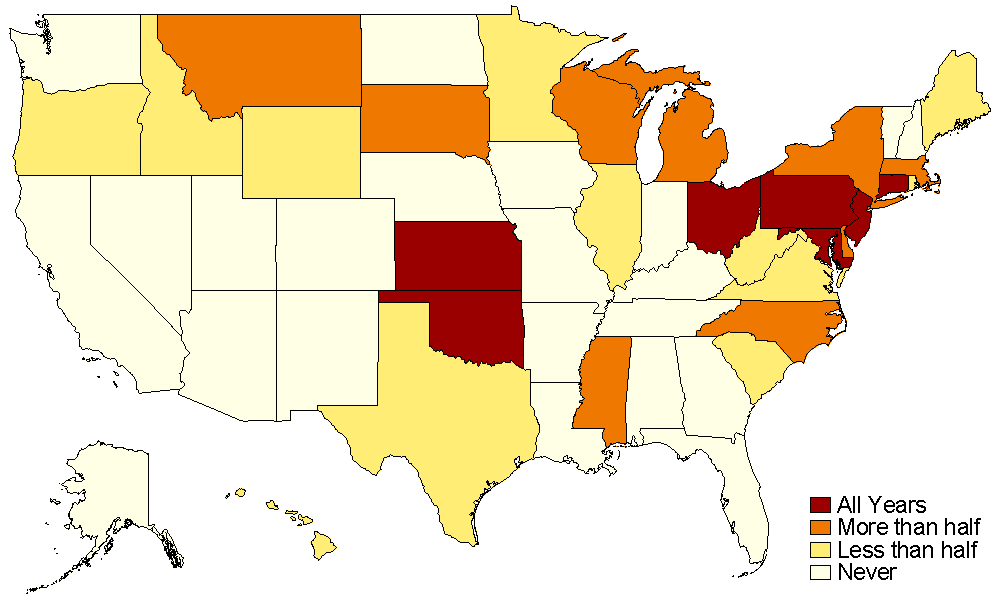
\includegraphics[width=.9\textwidth]{../Figures/Figure1_a.pdf}
	\label{fig:EImaps}
	\centering
	\caption*{Panel B. 2002-2017}
	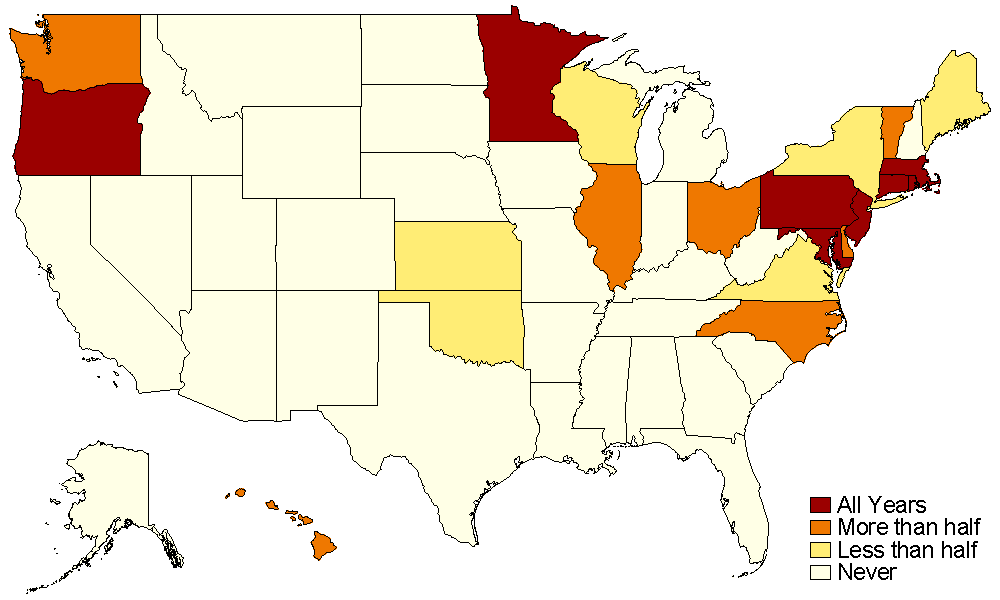
\includegraphics[width=.9\textwidth]{../Figures/Figure1_b.pdf}
	\end{center}
	\vspace{8pt}
    %\caption*{\footnotesize *Excluding ``pick-up'' taxes. See text for details.}
\end{figure}
\clearpage



\begin{figure}
	\centering
	\caption{Population of Forbes 400 by State}
	\label{fig:Stockmaps}
	\caption*{Panel A. 1982}
	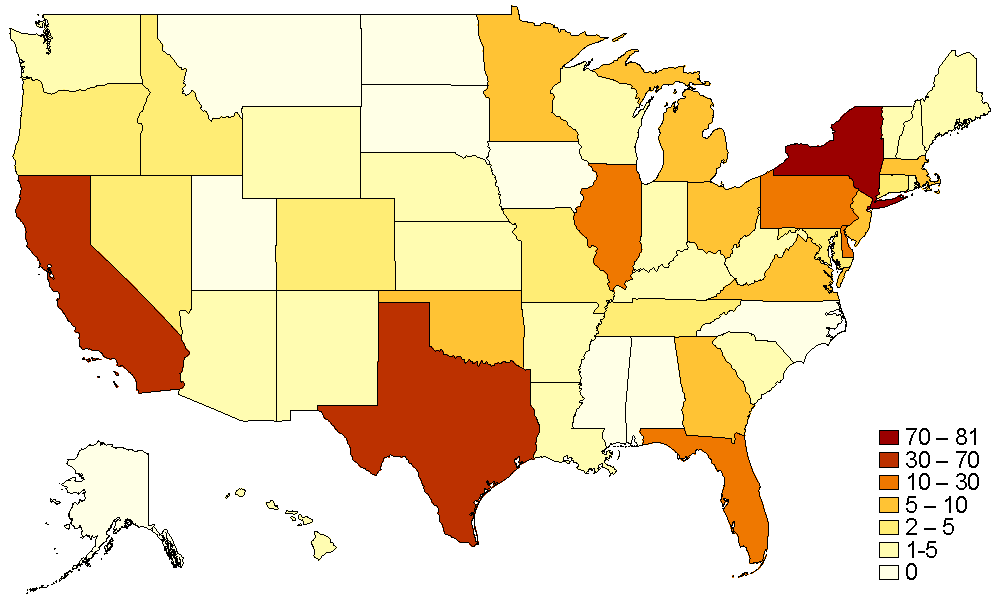
\includegraphics[width=.9\textwidth]{../Figures/Figure2_a.pdf}
	\centering
	\caption*{Panel B. 2017}
	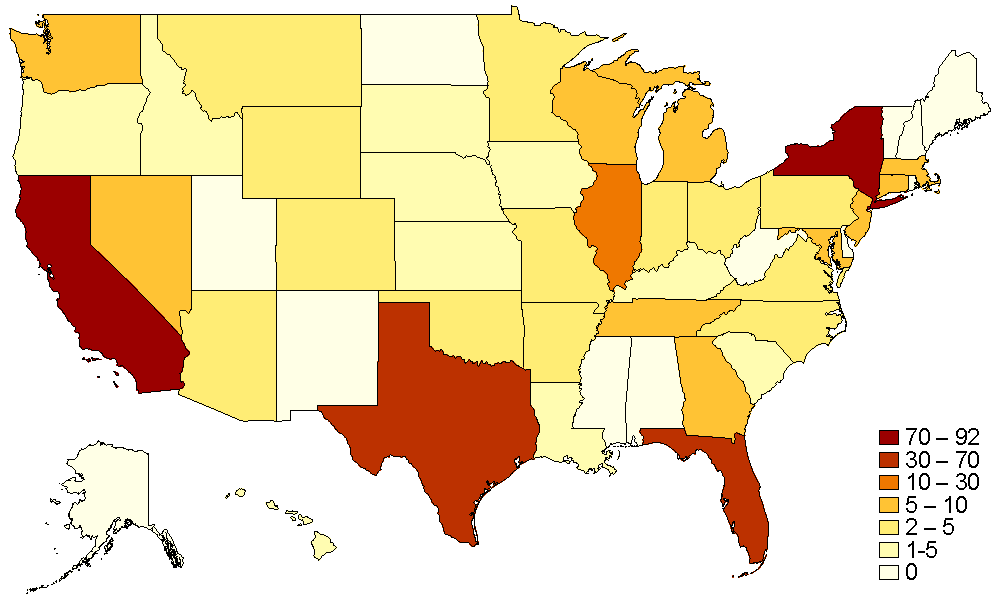
\includegraphics[width=.9\textwidth]{../Figures/Figure2_b.pdf}
\end{figure}
\vspace{10pt}
\clearpage



\begin{figure}
	\centering
	\caption{Impact of Billionaire Death on State Estate Tax Revenues\\Two Case Studies}	
	\caption*{Bud Walton of Arkansas, Died in 1995}
	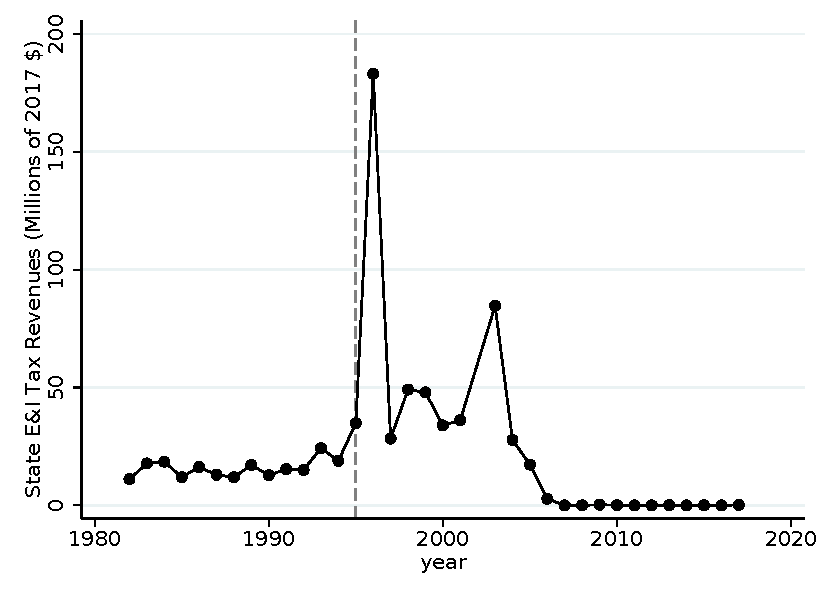
\includegraphics[width=.8\textwidth]{../Figures/Figure3_a.pdf}
    \vspace{10pt}
	\caption*{Edward Gaylord of Oklahoma, Died in 2003}
	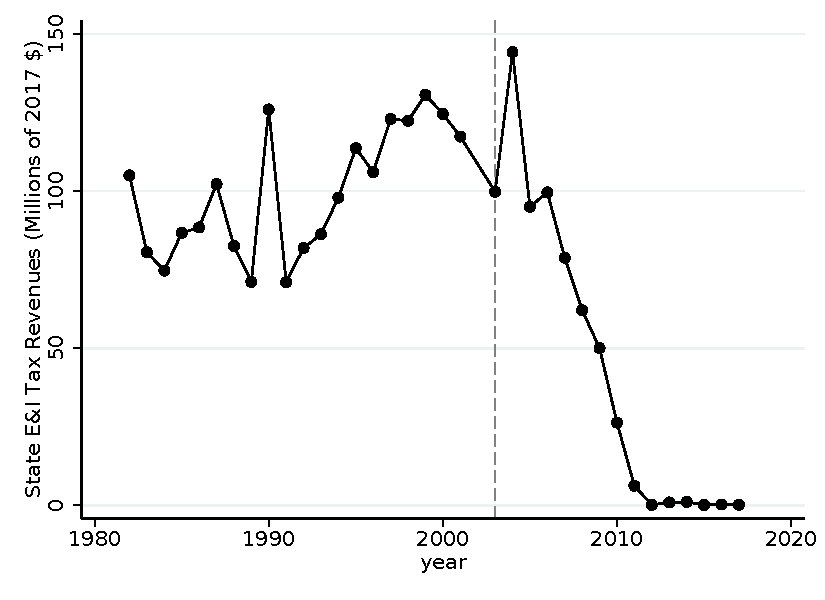
\includegraphics[width=.8\textwidth]{../Figures/Figure3_b.pdf}
\label{fig:case_studies}
\end{figure}

\clearpage
\begin{figure}
	\begin{center}
	\caption{Impact of Billionaire Death on State Estate Tax Revenues\\Event Study}
	\vspace{-12pt}
	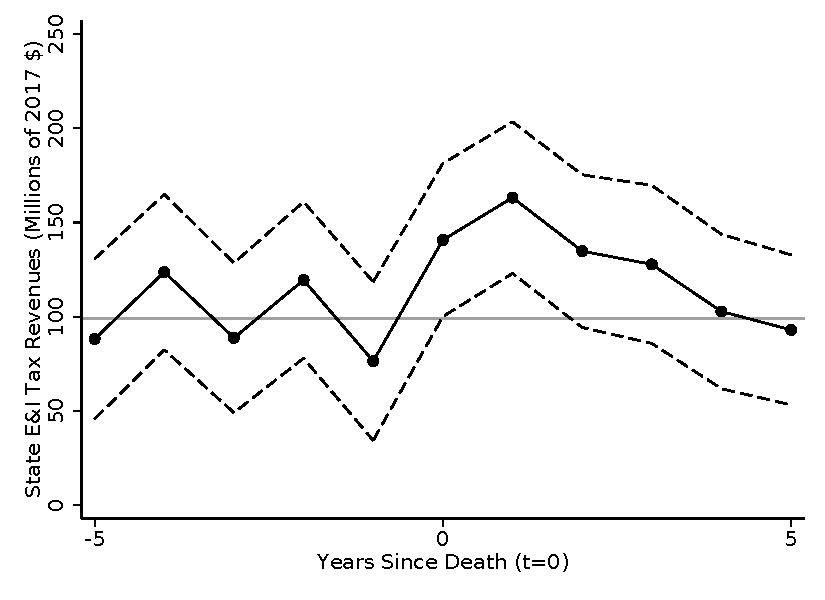
\includegraphics[width=.8\textwidth]{../Figures/Figure4.pdf}
    \label{fig:event_study}
	\end{center}
	\vspace{-16pt}
    \footnotesize{Notes: Horizontal line equals average coefficient over pre-death periods (-5 to -1). Dashed lines indicate 90\% confidence interval.}
\end{figure}

\vspace{8pt}
\begin{figure}
    \vspace{12pt}
	\begin{center}
	\caption{Share of Forbes 400 Living in a 2001 Estate Tax State}	
	\vspace{-8pt}
	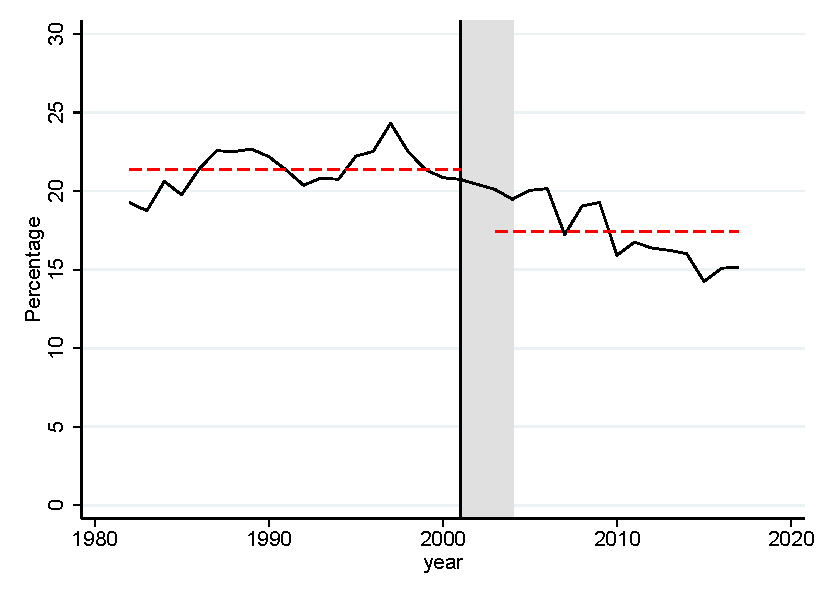
\includegraphics[width=.8\textwidth]{../Figures/Figure5.pdf}
    \label{fig:ShareIn2001ET}
	\end{center}
	\vspace{-16pt}
\footnotesize{Notes: Year 2002 is missing. Dashed horizontal lines are the mean before 2001 and after 2001.} 
\end{figure}
\clearpage




\begin{figure}
	\centering
	\caption{Probability of living in Estate Tax State By Age}	
	\caption*{Panel A. 1982-2001}
	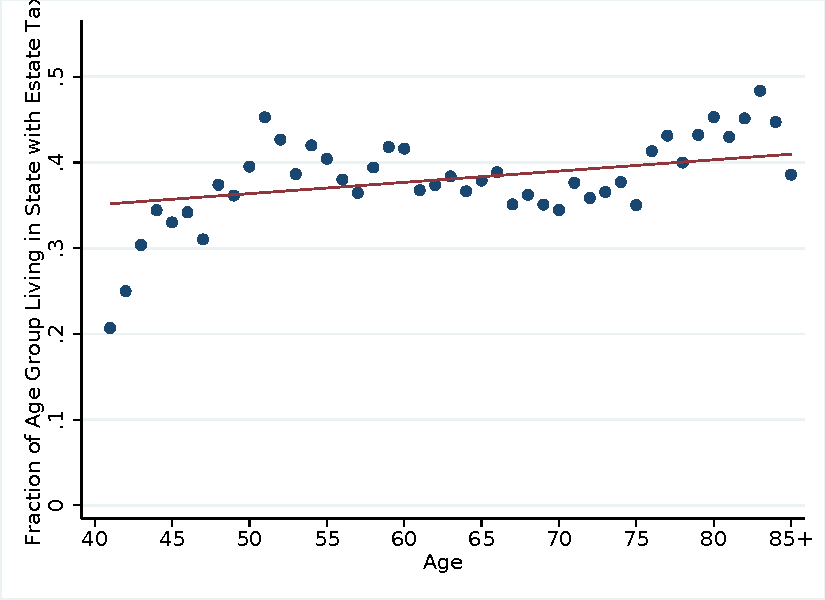
\includegraphics[width=.75\textwidth]{../Figures/Figure6_a.pdf}
	\caption*{Panel B. 2003-2017}
	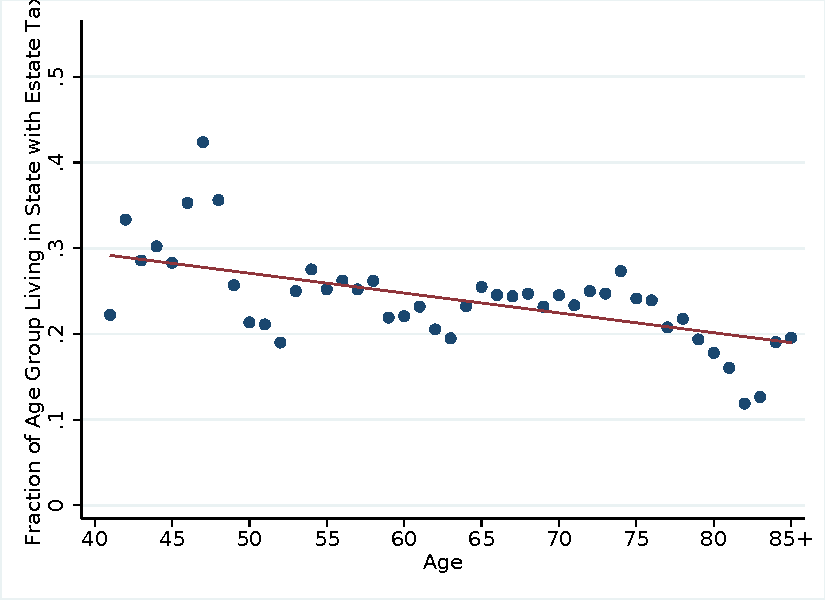
\includegraphics[width=.75\textwidth]{../Figures/Figure6_b.pdf}
	\caption*{\footnotesize Notes: Age Groups below 40 are excluded. Individuals above 85 are pooled and displayed at Age ``85+''. Note there is no data used for 2002 because Forbes did not report state of residence in that year.}
\label{fig:binscatterEI_Age}

\vspace{20cm}
\end{figure}

\clearpage


\begin{figure}
	\centering
	\caption{Estimated Age Gradient for Probability of Living in Estate Tax State}	
	\caption*{Year-by-Year Regressions}
	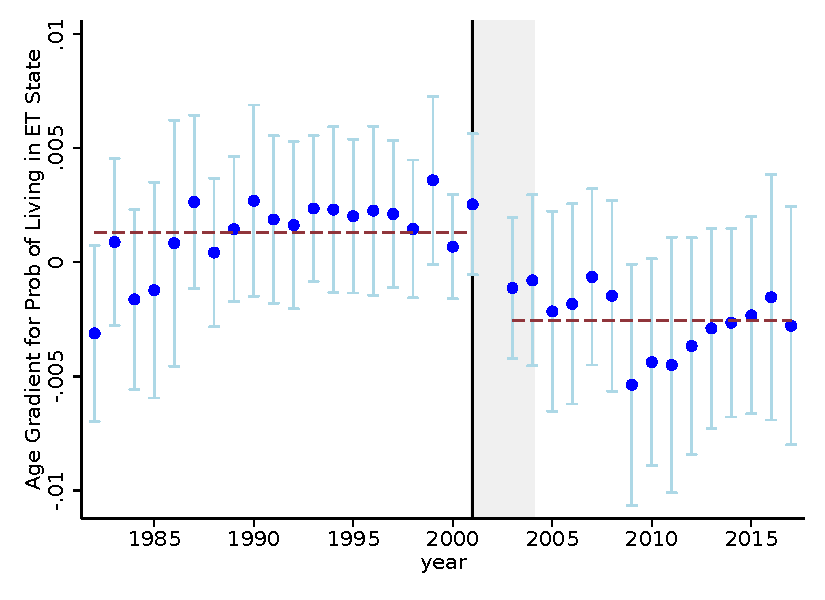
\includegraphics[width=.8\textwidth]{../Figures/Figure7.pdf}
	\caption*{\footnotesize Notes: Brackets indicate 90\% confidence intervals (clustered on state-year). Regressions include all individuals over 39 years old. Dashed horizontal lines are the means of the yearly age gradients over the pre-2002 and post-2002 periods. Note there is no age gradient for 2002 because Forbes did not report state of residence in that year.}
\label{fig:AgeGradientByYear}
%Notes: Dotted horizontal lines are the mean before 2001 and after 2001
\end{figure}



\clearpage





\begin{figure}
\centering
\caption{Probability of Moving Between ET States and Non-ET States}
	\caption*{Panel A. All}
	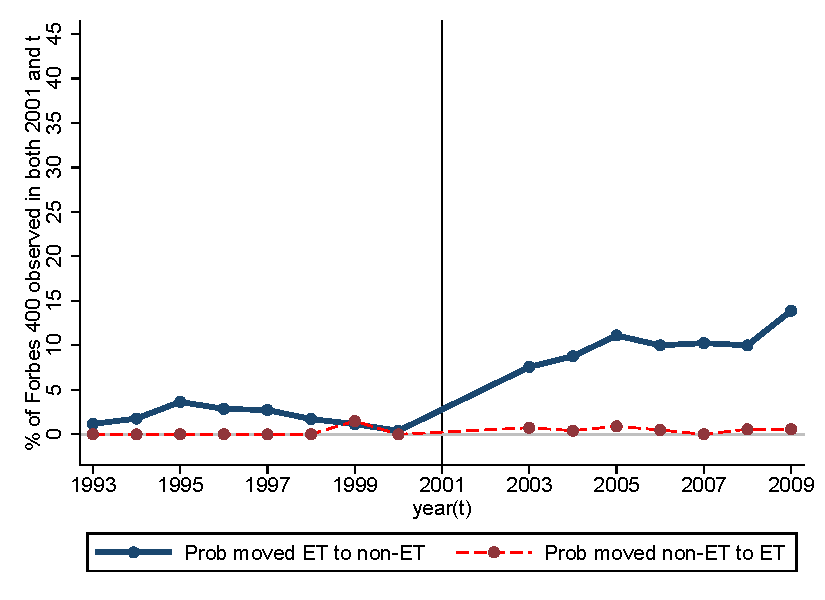
\includegraphics[width=.55\textwidth]{../Figures/Figure8_a.pdf}
	\caption*{Panel B. 65 and Over}
	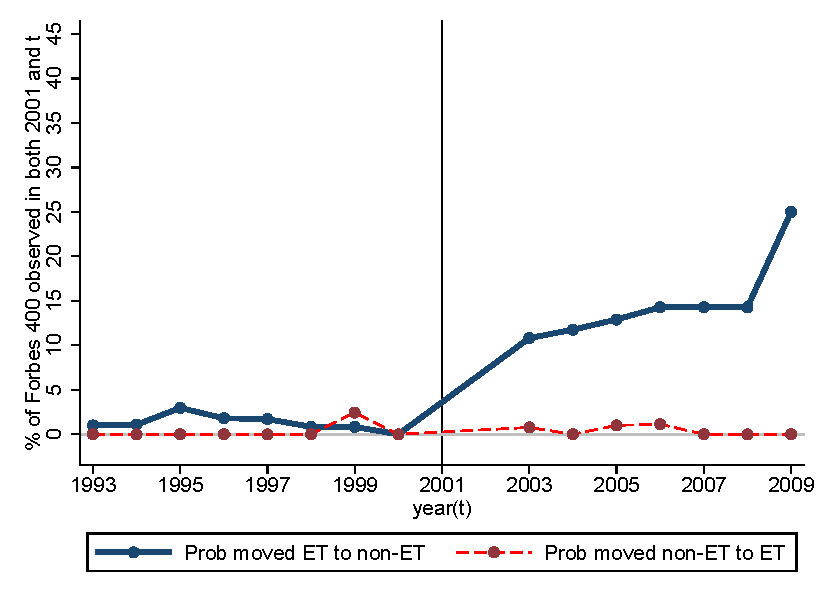
\includegraphics[width=.55\textwidth]{../Figures/Figure8_b.pdf}
	\caption*{Panel C. Under 65}
	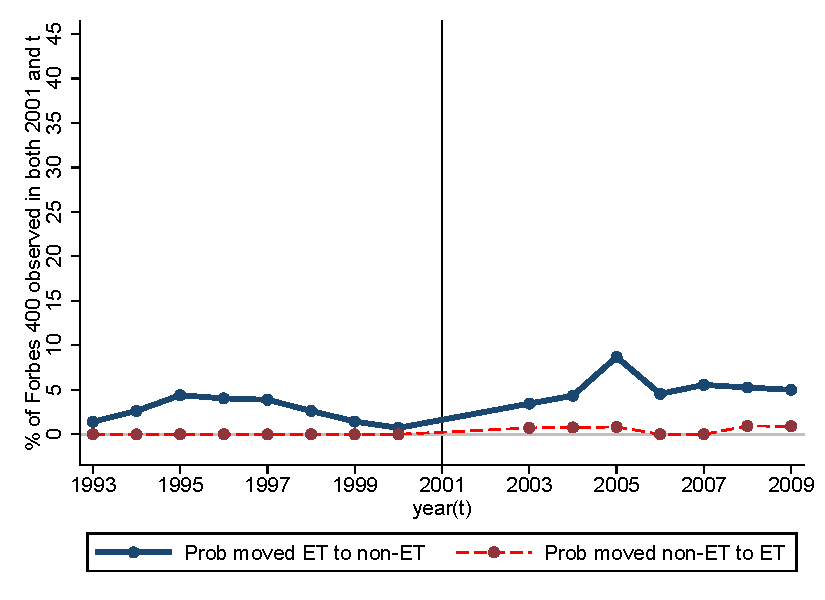
\includegraphics[width=.55\textwidth]{../Figures/Figure8_c.pdf}
	\caption*{\footnotesize Notes: The blue line is the probability of moving from a ET state to a non-ET state. The red line is the probability of moving from a non-ET state to an ET state. Year 2002 is missing. See text for details.}
\label{pre}
\end{figure}
\clearpage




%\begin{figure}
%\caption{Cost-Benefit By State, as of 2017}
%	\includegraphics[width=.85\textwidth]{../tables/CBratioAge_map_2017.pdf}
%
%\vspace{10cm}
%\end{figure}



%\clearpage

\noindent {\bf \large ONLINE APPENDIX for "Taxing Billionaires: Estate Taxes and the Geographical Location of the Ultra-Wealthy" by Enrico Moretti and Daniel J. Wilson -- Not For Publication}
\vspace{20pt}

\noindent {\bf \large ONLINE APPENDIX A -- Data Used in Cost-Benefit Calculations}
\vspace{10pt}

In this appendix, we discuss the data that we use in section \ref{all} to compute the costs and benefits of a broad-based estate tax on wealthy taxpayers.
We use equations (\ref{eq3}) and (\ref{eq4}).   
We need  state-by-state data or estimates on (1) the estate tax base ($(W_{as} N_{as}$) -- i.e., the total wealth of all state residents with wealth above the exemption level, (2) the income tax base for potential estate taxpayers ($(Y_{as} N_{as}$) -- i.e., the total income of all state residents with wealth above the exemption level, (3) the average effective tax rates on estate wealth ($\tau_s^{W}$) and income ($\tau_s^{Y}$) for potential estate taxpayers. 

\textbf{Estate tax base. }
In 2017, the federal estate tax applies to estate values above \$5.5 million for individuals and \$11 million for couples. Most current estate-tax states follow this federal exemption level, while some had lower exemptions. (The lowest is \$1 million in Massachusetts and Oregon (see \cite{michael2018survey}).
In our calculations, we use for simplicity the same exemption threshold  that applies U.S. federal estate tax 
and same degree of progressivity -- except with a 16\% top marginal rate, which is the top rate nearly all estate-tax states have currently. 

To estimate the potential estate tax base in each state, we start with IRS Statistics on Income (SOI) data on total estate values reported on federal estate tax returns by state of residence.\footnote{\url{https://www.irs.gov/statistics/soi-tax-stats-estate-tax-statistics-filing-year-table-2}.} Because the wealth by state on federal estate tax returns can be volatile from year to year, especially for small states, we use the average over 2015-2017 rather than just 2017. To fully utilize age-specific IRS data on income to wealth ratios discussed below, we apportion the statewide estate values to three broad age group (under 70, 70-79, and over 79) using national shares of estate tax returns by age group. Following the estate multiplier technique of \cite{kopczuk-saez:2004} and others, we estimate the underlying living population of wealthy taxpayers in each state by dividing the total estate values by the mortality rate for each age group from the Social Security Administration.\footnote{\url{https://www.ssa.gov/oact/STATS/table4c6.html}.} Given that mortality rates have been found to be considerably lower for the wealthy than for the general population, we adjust the mortality rates based on the mortality differentials provided in \cite{saez-zucman:2019}.   

\textbf{Income tax base.}
The income tax base for the population of potential estate taxpayers, by state and age group, can be estimated by multiplying the state-specific taxable estate tax values ($W_{as} N_{as}$) obtained above by the aggregate ratio of taxable income ($Y_a N_a$) to taxable estate value ($W_a N_a$) over all federal estate taxpayers:
%\begin{equation}
 $   Y_{as} N_{as} = W_{as} N_{as} \left(\frac{Y_a N_a}{W_a N_a}\right) $.
%\end{equation}
The national aggregates of $Y_a N_a$ and $W_a N_a$, by age group, are provided by the IRS Statistics on Income. Specifically, for 2008, the IRS matched all federal estate tax returns to the Form 1040 income tax returns filed by the decedent in the year prior to death. They report both taxable estate value and prior-year taxable income across taxpayers within each broad age group.\footnote{We add back spousal bequest deductions to taxable estate value because our cost estimates are based on revenues collected when the surviving spouse dies.} In aggregate, these taxpayers had taxable estate values of \$117.1 billion and prior-year taxable incomes of \$7.9 billion -- an income/wealth ratio of 0.074. The ratio falls with age (due primarily to labor income falling sharply over these three age groups): It is 0.103 for those under 70, 0.071 for ages 70 to 79, and 0.058 for those over 79.

\textbf{Average tax rates.}
For the average income tax rate, we use the top marginal tax rate, as we did in the previous section. Top income tax brackets among states generally start at incomes well below the income levels of individuals with wealth above the federal estate tax exemption (\$11 million for couples). Given that we seek to estimate the costs and benefits of states adopting an estate tax with the same degree of progressivity as the federal estate tax, albeit with a lower top rate (16\%), we need to take account of this progressivity when estimating the average effective estate tax rate. To estimate this average rate, we multiply the top marginal rate in state estate taxes, 16\%, by the ratio of the average tax rate to the top marginal tax rate in the federal estate tax. The federal top marginal rate in 2017 was 40\%. The average effective tax rate, based on 2017 IRS SOI data on total estate tax payments as a percentage of taxable estate values (adjusted for spousal deductions), was 25\%. Hence, we estimate the state average estate tax rate would be 16\%*(25/40) = 10\%.

%\textbf{Additional parameters.} For $T_a$ and $r$, we use the same parameters that we used for billionaires. 

\clearpage



%%%%%%%%%%%%%%%%%%%%%%%%%%%%%%%%%%%%%%%%%%%%%%%%%%%%%%%
% Appendix Tables and Figures
%%%%%%%%%%%%%%%%%%%%%%%%%%%%%%%%%%%%%%%%%%%%%%%%%%%%%%%
\setcounter {table} {0}
\setcounter {figure} {0}
\renewcommand{\thetable}{B\arabic{table}}
\renewcommand{\thefigure}{B\arabic{figure}}




%\graphicspath{{Figures/}}
\begin{table}
\begin{center}
\textbf{ONLINE APPENDIX B}

	\caption{\\Maximum Federal Credit Schedule for State Estate Taxes\\1954-2001}
		\scalebox{1} {
		\renewenvironment{table}[1][]{\ignorespaces}{\unskip}
        \begin{tabular}{ccc}
		Taxable Estate (\$)&Base Amount of Credit (\$)&Credit Rate on Excess (\%) \\
\midrule
100,000&0&0.8 \\
150,000&400&1.6 \\
200,000&1,200&2.4 \\
300,000&3,600&3.2 \\
500,000&10,000&4.0 \\
700,000&18,000&4.8 \\
900,000&27,600&5.6 \\
1,100,000&38,800&6.4 \\
1,600,000&70,800&7.2 \\
2,100,000&106,800&8.0 \\
2,600,000&146,800&8.8 \\
3,100,000&190,800&9.6 \\
3,600,000&238,800&10.4 \\
4,100,000&290,800&11.2 \\
5,100,000&402,800&12.0 \\
6,100,000&522,800&12.8 \\
7,100,000&650,800&13.6 \\
8,100,000&786,800&14.4 \\
9,100,000&930,800&15.2 \\
10,100,000&1,082,800&16.0 \\
\midrule

        \label{tab:fedcreditrates}
        \end{tabular}
	}
\end{center}
\vspace{-6pt}
\footnotesize{\qquad \qquad \qquad \quad Source: \cite{bakija/slemrod:2004}, Table 1}
\vspace{10cm}
\end{table}


\begin{table}
	\centering
	\caption{Probability of State Having an Estate Tax -- Linear Probability Model}
	\scalebox{0.8}{
		\renewenvironment{table}[1][]{\ignorespaces}{\unskip}
		{
\def\sym#1{\ifmmode^{#1}\else\(^{#1}\)\fi}
\begin{tabular}{l*{3}{c}}
\hline\hline
                &\multicolumn{1}{c}{(1)}&\multicolumn{1}{c}{(2)}&\multicolumn{1}{c}{(3)}\\
                &\multicolumn{1}{c}{Estate Tax Indicator}&\multicolumn{1}{c}{Estate Tax Indicator}&\multicolumn{1}{c}{Estate Tax Indicator}\\
\hline
Top PIT Rate    &  0.00697         &   0.0119         &   0.0486\sym{*}  \\
                & (0.0228)         & (0.0243)         & (0.0282)         \\
[1em]
Top Corp. Income Tax (CIT) Rate&    4.595\sym{*}  &    3.994         &    3.977         \\
                &  (2.480)         &  (2.576)         &  (3.187)         \\
[1em]
Log Change in real GDP&-0.0000390         &0.00000809         &-0.000148         \\
                &(0.000357)         &(0.000492)         &(0.000322)         \\
[1em]
Top PIT Rate X post-2001&   0.0157         &   0.0116         &  0.00390         \\
                & (0.0231)         & (0.0234)         & (0.0211)         \\
[1em]
Top CIT Rate X post-2001&   -1.116         &   -0.212         &    1.010         \\
                &  (2.749)         &  (2.919)         &  (3.066)         \\
[1em]
GDP Change X post-2001&-0.00000228         & 0.000274         & 0.000267         \\
                &(0.000224)         &(0.000610)         &(0.000620)         \\
[1em]
Constant        &   0.0496         &    0.225         &    0.213         \\
                &  (0.343)         &  (0.409)         &  (0.323)         \\
\hline
Observations    &     1333         &     1333         &     1333         \\
State Fixed Effects         &       No         &       No         &      Yes         \\
Year Fixed Effects          &       No         &      Yes         &      Yes         \\
\hline \hline
\multicolumn{3}{l}{\footnotesize Standard errors (clustered by state) in parentheses.}\\
\multicolumn{3}{l}{\footnotesize \sym{*} \(p<0.10\), \sym{**} \(p<0.05\), \sym{***} \(p<0.01\)}  \end{tabular} }

		\unskip
	}
\label{tab:ETadopt}
\end{table}
\clearpage


\begin{center}
\begin{table}
	\caption{Summary Statistics}
	\vspace{10pt}

	\begin{center}
	\caption*{Panel A. Individual-by-Year Observations. 1982 -- 2017}
	\scalebox{0.8} {
		\renewenvironment{table}[1][]{\ignorespaces}{\unskip}
		{
\def\sym#1{\ifmmode^{#1}\else\(^{#1}\)\fi}
\begin{tabular}{l*{1}{ccccc}}
\hline\hline
                    &      Mean&              Median&Standard Deviation&             Minimum&   Maximum\\
\hline
Age                 &     64.31&               65.00&     13.11&               23.00&     96.00\\
Net Worth (billions, 2017 dollars)&      3.02&                1.60&      5.73&                0.19&    125.06\\
\hline
Observations        &     13432&                    &          &                    &          \\
\hline\hline
\end{tabular}
}

		\unskip
	}
	\end{center}
	\vspace{20pt}

	\begin{center}
	\caption*{Panel B. Distribution of Net Worth -- 2017}
	\scalebox{0.8} {
		\renewenvironment{table}[1][]{\ignorespaces}{\unskip}
{
	\def\sym#1{\ifmmode^{#1}\else\(^{#1}\)\fi}
	\begin{tabular}{l*{1}{ccccccc}}
		\hline\hline
		
		
		
&1st&10th&25th&50th&75th&90th&99th \\
\midrule
Net Worth (bill)&2.0&2.2&2.7&3.7&5.5&12.0&71.0 \\
\end{tabular}


}
		
		 \unskip
           }
	   
	\end{center}
	\vspace{10pt}

	\begin{center}
	\caption*{Panel C. State-by-Year Observations.  1982 -- 2017}
	\scalebox{0.8} {
		\renewenvironment{table}[1][]{\ignorespaces}{\unskip}
		{
\def\sym#1{\ifmmode^{#1}\else\(^{#1}\)\fi}
\begin{tabular}{l*{1}{ccccc}}
\hline\hline
                    &      Mean&              Median&Standard Deviation&             Minimum&   Maximum\\
\hline
Population of Forbes 400&      7.68&                3.00&     15.07&                0.00&     98.00\\
Net Worth (billions 2017 dollars)&     22.63&                5.86&     53.36&                0.00&    617.80\\
Estate Tax Indicator&      0.32&                0.00&      0.47&                0.00&      1.00\\
Top PIT Rate        &      4.86&                5.40&      2.96&                0.00&     14.10\\
\hline
Observations        &      1750&                    &          &                    &          \\
\hline\hline
\end{tabular}
}

		\unskip
	}
	\end{center}

\label{tab:summstats}
\end{table}
\end{center}

\clearpage


\begin{table}
	\caption{Forbes 400 by Consolidated Metro Area (Top 40), 2017}
	\centering
		\scalebox{0.81} {
        \begin{tabular}{lccc}
		& Forbes Population & Mean Wealth & 1982-2017 Change\\City & in 2017& in 2017 (mil) & in Forbes Population\\
\midrule
Atlanta-Sandy Springs-Gainesville, GA-AL&9&4767&2 \\
Austin-Round Rock-Marble Falls, TX&4&8025&4 \\
Birchwood&1&4200&1 \\
Bloomington, IN&1&7500&1 \\
Boston-Worcester-Manchester, MA-RI-NH&8&5988&-2 \\
Chicago-Naperville-Michigan City, IL-IN-WI&14&3443&-2 \\
Columbia, MO&2&6800&2 \\
Dallas-Fort Worth, TX&18&5950&-9 \\
Denver-Aurora-Boulder, CO&4&9900&-1 \\
Detroit-Warren-Flint, MI&3&4400&-1 \\
Fayetteville-Springdale-Rogers, AR-MO&4&20375&3 \\
Houston-Baytown-Huntsville, TX&11&4464&-10 \\
Indianapolis-Anderson-Columbus, IN&2&2700&0 \\
Jackson, WY&4&11700&4 \\
Kalamazoo-Portage, MI&2&3950&0 \\
Knoxville-Sevierville-La Follette, TN&2&3050&2 \\
Las Vegas-Paradise-Pahrump, NV&7&7471&4 \\
Los Angeles-Long Beach-Riverside, CA&31&4806&3 \\
Miami-Fort Lauderdale-Pompano Beach, FL&25&4416&13 \\
Milwaukee-Racine-Waukesha, WI&4&3800&3 \\
Minneapolis-St. Paul-St. Cloud, MN-WI&2&4100&-5 \\
Naples-Marco Island, FL&3&5033&2 \\
Nashville-Davidson--Murfreesboro--Columbia, TN&4&4275&3 \\
New York-Newark-Bridgeport, NY-NJ-CT-PA&80&6368&-9 \\
Oklahoma City-Shawnee, OK&3&7867&-2 \\
Omaha-Council Bluffs-Fremont, NE-IA&2&41100&1 \\
Philadelphia-Camden-Vineland, PA-NJ-DE-MD&5&3500&-16 \\
Phoenix-Mesa-Glendale, AZ&5&2780&5 \\
Portland-Vancouver-Hillsboro, OR-WA&2&14450&0 \\
Raleigh-Durham-Cary, NC&2&6700&2 \\
Rochester-Batavia-Seneca Falls, NY&2&2850&2 \\
San Diego-Carlsbad-San Marcos, CA&2&3750&-2 \\
San Jose-San Francisco-Oakland, CA&54&8154&37 \\
Santa Barbara-Santa Maria-Goleta, CA&2&4250&2 \\
Seattle-Tacoma-Olympia, WA&8&29775&7 \\
St. Louis-St. Charles-Farmington, MO-IL&2&5450&1 \\
Tampa-St. Petersburg-Clearwater, FL&4&2375&3 \\
Tulsa-Bartlesville, OK&2&5350&0 \\
Washington-Baltimore-Northern Virginia, DC-MD-VA-WV&10&5490&4 \\
Average&9&7470&1 \\

        \end{tabular}
        }
\label{tab3}
\end{table}



%\begin{landscape}
\tiny{
\begin{longtable}{l l l l l l}
			\caption{State of Deaths and State of Residence Reported by Forbes}\\ 
			\hline 
		Name &Death &Death &Obituary &Forbes &Notes\\ 
		  &Year &State &Res. State &Res. State & \\ [0.5ex]
		\hline
		
		Liliore Green Rains&1985&CA&CA&CA&\\
		Mary Belin Du Pont Faulkner&1985&MA&MA&MA&\\
		Abram Nicholas Pritzker&1986&IL&&IL&\\
		David Whitmire Hearst&1986&CA&CA&CA&\\
		Gordon Barton Mclendon&1986&TX&TX&TX&\\
		Howard Vollum&1986&OR&OR&OR&\\
		Arnold Bernhard&1987&NY&NY/CT&CT&\\
		Burton Green Bettingen&1987&CA&CA&CA&\\
		Henry Ford II&1987&MI&MI&FL&\\
		Henry John Heinz II&1987&FL&PA&PA&Died at winter home.\\
		Paul Kalmanovitz&1987&CA&CA&CA&\\
		Ruth Chandler Von Platen&1987&CA&CA&CA&\\
		Sol Goldman&1987&NY&NY&NY&\\
		John Wilmer Galbreath&1988&OH&OH&OH&\\
		Lawrence Arthur Wien&1988&CT&CT/NY/FL&NY&\\
		Pierre Samuel Du Pont&1988&DE&DE&DE&\\
		Henry Crown&1990&IL&IL &IL&\\
		Mark Goodson&1992&NY&NY&NY&\\
		Edward John Debartolo&1994&OH&OH&OH&\\
		Milton Jack Petrie&1994&NY&NY&NY&\\
		Albert B Alkek&1995&TX&TX&TX&\\
		Alpheus Lee Ellis&1995&FL&FL&FL&\\
		Erskine Bronson Ingram&1995&TN&TN&TN&\\
		James Lawrence Walton&1995&AR&FL&AR&Died on fishing trip.\\
		John Jeffry Louis&1995&IL&IL&IL&\\
		Joseph R Coulter&1995&FL&FL&FL&\\
		Walter A Haas&1995& CA&CA&CA&\\
		Bob John Magness&1996&CO&VA&&UVA hospital.\\
		Daniel James Terra&1996&WA&IL/WA/France&IL&\\
		David Packard&1996&CA&CA&CA&\\
		Louis Larrick Ward&1996&MO&MO&MO&\\
		Claude Bernard Pennington&1997&LA&LA&LA&\\
		Herbert Allen&1997&NY&NY&NY&\\
		Jack Kent Cooke&1997&DC&DC&VA&\\
		Roberto Crispulo Goizueta&1997&GA&GA&GA&\\
		Betsey Cushing Roosevelt Whitney&1998&NY&NY &NY&\\
		Dwight Lyman Stuart&1998&CA&CA&CA&\\
		John William Berry&1998&OH&OH&OH&\\
		William Michael Cafaro&1998&OH&OH&OH&\\
		Curtis Leroy Carlson&1999&MN&MN&MN&\\
		Forrest Edward Mars Sr&1999&FL&FL&NV&\\
		Henry Earl Singleton&1999&CA&CA&CA&\\
		Jay Arthur Pritzker&1999&IL&IL&IL&\\
		Leon Hess&1999&NY&NY&NJ&\\
		Paul Mellon&1999&VA&VA&VA&\\
		Ruth Ray Hunt&1999&TX&TX&TX&\\
		Ted Arison&1999&Tel Aviv&Tel Aviv&FL&\\
		Bill Daniels&2000&CA&CA&CO&Died in hospital.\\
		Marshall Naify&2000&CA&CA&CA&\\
		Randolph Apperson Hearst&2000&NY&NY&NY&\\
		Edmund Wattis Littlefield&2001&CA&CA&CA&\\
		Larry Fisher&2001&FL&FL/ NY&NY&\\
		Malcom Purcell Mclean&2001&NY&NY&NY&\\
		Michel Fribourg&2001&NY&NY&NY&\\
		Reese Mcintosh Rowling&2001&TX&TX&TX&\\
		William Redington Hewlett&2001&CA&CA&CA&\\
		Alfred Lerner&2002&OH&OH&OH&\\
		Kathryn Mccurry Albertson&2002&ID&ID&ID&\\
		Millicent V Boudjakdji&2002&LA&LA&CA&\\
		Robert Henry Dedman&2002&TX&TX&TX&\\
		Victor Posner&2002&FL&FL&FL&\\
		Walter Hubert Annenberg&2002&PA&PA/CA&PA&\\
		Edward Lewis Gaylord&2003&OK&OK&OK&\\
		Joan Beverly Kroc&2003&CA&CA&CA&\\
		Laurence Alan Tisch&2003&NY&NY&NY&\\
		Samuel Jayson LeFrak&2003&NY&NY&NY&\\
		Charles B Benenson&2004&FL&NY&NY&Died suddenly.\\
		Jay Van Andel&2004&MI&MI&MI&\\
		Laurance Spelman Rockefeller&2004&NY&NY&NY&\\
		Marvin Harold Davis&2004&CA&CA&CA&\\
		Samuel Curtis Johnson&2004&WI&WI&WI&\\
		Susan Thompson Buffett&2004&CA&WY&CA&Died on vacation.\\
		Franklin Parsons Perdue&2005&MD&MD&MD&\\
		Jackson Thomas Stephens&2005&AR&AR&AR&\\
		Peter E Haas&2005&CA&CA&CA&\\
		Preston Robert Tisch&2005&NY&NY&NY&\\
		James R Cargill&2006&MN&MN&MN&\\
		Lamar Hunt&2006&TX&TX&TX&\\
		Margaret Anne Cargill&2006&CA&CA&CA&\\
		Raymond J Noorda&2006&UT&UT&UT&\\
		Robert Edward Rich&2006&FL&FL&FL&\\
		Barbara Cox Anthony&2007&HI&GA/HI&HI&\\
		Helen Walton&2007&AR&AR&AR&\\
		James Martin Moran&2007&FL&FL&FL&\\
		Margaret Hunt Hill&2007&TX&TX&TX&\\
		James LeVoy Sorenson&2008&UT&UT&UT&\\
		John Hugh Macmillan&2008&FL&FL&FL&\\
		John Richard Simplot&2008&ID&ID&ID&\\
		Carl Ray Pohlad&2009&MN&MN&MN&\\
		Frank Batten&2009&VA&VA&VA&\\
		Melvin Simon&2009&IN&IN&IN&\\
		Samuel J Heyman&2009&NY&NY, FL, CN&NY&Died after surgery.\\
		Trammell Crow&2009&TX&TX&TX&\\
		William Morse Davidson&2009&MI&MI&MI&\\
		Dolph Briscoe&2010&TX&TX&TX&\\
		John Werner Kluge&2010&VA&VA&FL&\\
		Paul Milstein&2010&NY&NY&NY&\\
		Richard N Goldman&2010&CA&CA&CA&\\
		Cargill Macmillan&2011&CA&CA&CA&\\
		Carl Henry Lindner&2011&OH&OH&OH&\\
		Jack N Mandel&2011&OH&OH&OH&\\
		Jean Ellen Du Pont Sheehan&2011&DE&DE&FL&\\
		John Charles Haas&2011&PA&PA&PA&\\
		John Edward Anderson&2011&CA&CA&CA&\\
		Malcolm Green Chace&2011&MA&MA&RI&\\
		Robert Alan Pritzker&2011&IL&IL&IL&\\
		William Alfred Cook&2011&IN&IN&IN&\\
		Albert Lee Ueltschi&2012&FL&FL&FL&\\
		Donald J Schneider&2012&WI&WI&WI&\\
		Barbara Piasecka Johnson&2013&Poland&Italy, Poland, Monaco&NJ&\\
		Edgar Miles Bronfman&2013&NY&NY&NY&\\
		Harold Clark Simmons&2013&TX&TX&TX&\\
		Leonard Samuel Skaggs&2013&UT&UT&UT&\\
		Robert Earl Holding&2013&UT&&ID&Res. state unclear.\\
		James Edwards Stowers&2014&MO&MO&MO&\\
		Malcolm Glazer&2014&FL&FL&FL&\\
		Nelson Bunker Hunt&2014&TX&TX&TX&\\
		Patrick Joseph Mcgovern&2014&NH&CA&NH&\\
		Kirk Kerkorian&2015&CA&CA&CA&\\
		Michael Birck&2015&IL&IL&IL&\\
		Ralph J Roberts&2015&PA&PA&PA&\\
		Forrest Edward Mars Jr&2016&WY&WA&WY&\\
		Jack Crawford Taylor&2016&MO&MO&MO&\\
		Joseph C Mandel&2016&FL&OH&OH&Died at winter home.\\
		Leandro Rizzuto&2017&FL&FL&WY&\\
		Michael Ilitch&2017&MI&MI&MI&\\
		Samuel Irving Newhouse&2017&NY&NY&NY&\\
		Charles B Wang&2018&NY&NY&NY&\\
		\hline
\label{deaths}
\end{longtable}
%\end{landscape}
}	

\clearpage


\begin{table}
\centering
	\caption{Robustness}
%	\vspace{4pt}
	\caption*{Panel A. Difference-in-Difference}
	\scalebox{0.8} {
		\renewenvironment{table}[1][]{\ignorespaces}{\unskip}
		{
\def\sym#1{\ifmmode^{#1}\else\(^{#1}\)\fi}
\begin{tabular}{l*{4}{c}}
\hline\hline
                &\multicolumn{1}{c}{(1)}&\multicolumn{1}{c}{(2)}&\multicolumn{1}{c}{(3)}&\multicolumn{1}{c}{(4)}\\
                &\multicolumn{1}{c}{Top 100}&\multicolumn{1}{c}{Top200}&\multicolumn{1}{c}{Top300}&\multicolumn{1}{c}{10+ Obs}\\
\hline
ET-state X post-2001&   -0.553\sym{***}&   -1.307\sym{***}&   -1.902\sym{***}&   -2.182\sym{***}\\
                &  (0.105)         &  (0.195)         &  (0.388)         &  (0.522)         \\
[1em]
ET-state        &   0.0599         &    0.500         &    0.911\sym{*}  &    0.944\sym{***}\\
                &  (0.199)         &  (0.318)         &  (0.466)         &  (0.356)         \\
\hline
Observations    &     1575         &     1610         &     1680         &     1575         \\
Semi-elasticity            &    -.338         &    -.327         &    -.361         &      -.4         \\
\quad \textit{Std. Error}          &     .064         &     .049         &     .073         &     .096         \\
\hline \hline
\multicolumn{5}{l}{\footnotesize Driscoll-Kraay (with 10-year bandwidth) standard errors in parentheses.} \\
\multicolumn{5}{l}{\footnotesize All regressions include state and year fixed effects.} \\
\multicolumn{5}{l}{\footnotesize \sym{*} \(p<0.10\), \sym{**} \(p<0.05\), \sym{***} \(p<0.01\)}  \end{tabular} }

	}
	
%	\vspace{4pt}
	\caption*{Panel B. Triple-Difference}
	\scalebox{0.8} {
		\renewenvironment{table}[1][]{\ignorespaces}{\unskip}
		{
\def\sym#1{\ifmmode^{#1}\else\(^{#1}\)\fi}
\begin{tabular}{l*{4}{c}}
\hline\hline
                &\multicolumn{1}{c}{(1)}&\multicolumn{1}{c}{(2)}&\multicolumn{1}{c}{(3)}&\multicolumn{1}{c}{(4)}\\
                &\multicolumn{1}{c}{Top 100}&\multicolumn{1}{c}{Top200}&\multicolumn{1}{c}{Top300}&\multicolumn{1}{c}{10+ Obs}\\
\hline
ET-state X post-2001 X old&   -0.762\sym{***}&   -0.808\sym{***}&   -1.127\sym{***}&   -1.178\sym{**} \\
                &  (0.166)         &  (0.265)         &  (0.346)         &  (0.471)         \\
[1em]
ET-state X old  &    0.245\sym{***}&    0.272\sym{***}&    0.411\sym{***}&    0.440\sym{**} \\
                & (0.0779)         & (0.0749)         & (0.0990)         &  (0.188)         \\
[1em]
ET-state X post-2001&    0.104         &   -0.250\sym{*}  &   -0.388\sym{**} &   -0.502\sym{**} \\
                & (0.0842)         &  (0.130)         &  (0.152)         &  (0.240)         \\
[1em]
old X post-2001 &    0.893\sym{***}&    1.181\sym{***}&    1.603\sym{***}&    2.166\sym{***}\\
                &  (0.121)         &  (0.242)         &  (0.301)         &  (0.537)         \\
[1em]
ET-state        &  -0.0926         &    0.114         &    0.250         &    0.252         \\
                & (0.0888)         &  (0.147)         &  (0.224)         &  (0.194)         \\
[1em]
old             &   -0.206\sym{***}&   -0.352\sym{***}&   -0.499\sym{***}&   -0.459\sym{*}  \\
                & (0.0586)         & (0.0843)         &  (0.149)         &  (0.244)         \\
\hline
Observations    &     3150         &     3220         &     3360         &     3150         \\
Semi-elasticity, Young      &     .036         &    -.086         &    -.133         &    -.173         \\
\quad \textit{Std. Error}    &     .029         &     .045         &     .052         &     .083         \\
Semi-elasticity, Old        &    -.603         &    -.465         &     -.49         &    -.499         \\
\quad \textit{Std. Error}      &     .101         &     .085         &     .108         &      .13         \\
\hline \hline
\multicolumn{5}{l}{\footnotesize Driscoll-Kraay (with 10-year bandwidth) standard errors in parentheses. All regressions} \\
\multicolumn{5}{l}{\footnotesize include year fixed effects. State fixed effects are absorbed by old-young differencing.} \\
\multicolumn{5}{l}{\footnotesize \sym{*} \(p<0.10\), \sym{**} \(p<0.05\), \sym{***} \(p<0.01\)}  \end{tabular} }

	}

%	\vspace{4pt}
	\caption*{Panel C. Linear Probability Model}
	\scalebox{0.8} {
		\renewenvironment{table}[1][]{\ignorespaces}{\unskip}
		{
\def\sym#1{\ifmmode^{#1}\else\(^{#1}\)\fi}
\begin{tabular}{l*{4}{c}}
\hline\hline
                &\multicolumn{1}{c}{(1)}&\multicolumn{1}{c}{(2)}&\multicolumn{1}{c}{(3)}&\multicolumn{1}{c}{(4)}\\
                &\multicolumn{1}{c}{Top 100}&\multicolumn{1}{c}{Top200}&\multicolumn{1}{c}{Top300}&\multicolumn{1}{c}{10+ Obs}\\
\hline
Age X post-2001 & -0.00563\sym{***}& -0.00362\sym{***}& -0.00295\sym{***}& -0.00337\sym{***}\\
                &(0.000899)         &(0.000806)         &(0.000719)         &(0.000848)         \\
[1em]
Age             &  0.00273\sym{***}&  0.00127\sym{**} & 0.000987\sym{*}  &  0.00134\sym{**} \\
                &(0.000914)         &(0.000632)         &(0.000565)         &(0.000653)         \\
\hline
Observations    &     3276         &     6465         &     9686         &     9714         \\
\hline \hline
\multicolumn{5}{l}{\footnotesize Driscoll-Kraay standard errors in parentheses.} \\
\multicolumn{5}{l}{\footnotesize All regressions include state and year fixed effects.} \\
\multicolumn{5}{l}{\footnotesize \sym{*} \(p<0.10\), \sym{**} \(p<0.05\), \sym{***} \(p<0.01\)}  \end{tabular} }

	}
\label{tab:RestrictedSamples}
\end{table}

\clearpage

\begin{table}
	\centering
	\caption{Cost-Benefit Results Under Alternative Assumptions}
	\caption*{Panel A: Billionaires Estate Tax}
	\scalebox{0.9} {
		\renewenvironment{table}[1][]{\ignorespaces}{\unskip}
		% matrix: R1 file: ../Tables/TableB7_a.tex  15 Dec 2021 15:33:16
\begin{table}[htbp]
\begin{tabular}{|l|c|c|c|c|c|c|}\hline  
 & Baseline  & Alt 1  & Alt 2  & Alt 3  & Alt 4  & Alt 5  \\ \hline  
ET States (10) &   . &   . &   . &   . &   . &   . \\ \hline 
Average CB ratio & 0.49 & 0.18 & 0.73 & 0.41 & 0.58 & 0.23 \\ \hline 
Number with CB$\geq$1 & 1.00 & 0.00 & 2.00 & 0.00 & 1.00 & 0.00 \\ \hline 
r4 &   . &   . &   . &   . &   . &   . \\ \hline 
Non-ET States (28) &   . &   . &   . &   . &   . &   . \\ \hline 
Average CB ratio & 0.31 & 0.13 & 0.48 & 0.27 & 0.35 & 0.14 \\ \hline 
Number with CB$\geq$1 & 1.00 & 0.00 & 1.00 & 0.00 & 1.00 & 0.00 \\ \hline 
Average CB ratio &   . &   . &   . &   . &   . &   . \\ \hline 
Number with CB$\geq$1 &   . &   . &   . &   . &   . &   . \\ \hline 
r10 & 0.36 & 0.14 & 0.55 & 0.31 & 0.42 & 0.17 \\ \hline 
All States (38) & 2.00 & 0.00 & 3.00 & 0.00 & 2.00 & 0.00 \\ \hline 
  \end{tabular}
\end{table}

		\unskip
	}
	\vspace{10pt}
	\caption*{Panel B: Broad Estate Tax}
	\scalebox{0.9} {
		\renewenvironment{table}[1][]{\ignorespaces}{\unskip}
		% matrix: R2 file: ../Tables/TableB7_b.tex  15 Dec 2021 15:33:16
\begin{table}[htbp]
\begin{tabular}{|l|c|c|c|c|c|c|}\hline  
 & Baseline  & Alt 1  & Alt 2  & Alt 3  & Alt 4  & Alt 5  \\ \hline  
ET States (14) &   . &   . &   . &   . &   . &   . \\ \hline 
Average CB ratio & 0.71 & 0.28 & 1.05 & 0.61 & 0.83 & 0.71 \\ \hline 
Number with CB$\geq$1 & 3.00 & 0.00 & 9.00 & 1.00 & 5.00 & 3.00 \\ \hline 
r4 &   . &   . &   . &   . &   . &   . \\ \hline 
Non-ET States (36) &   . &   . &   . &   . &   . &   . \\ \hline 
Average CB ratio & 0.45 & 0.18 & 0.66 & 0.38 & 0.52 & 0.45 \\ \hline 
Number with CB$\geq$1 & 1.00 & 0.00 & 5.00 & 1.00 & 1.00 & 1.00 \\ \hline 
Average CB ratio &   . &   . &   . &   . &   . &   . \\ \hline 
Number with CB$\geq$1 &   . &   . &   . &   . &   . &   . \\ \hline 
r10 & 0.53 & 0.21 & 0.78 & 0.45 & 0.62 & 0.53 \\ \hline 
All States (50) & 4.00 & 0.00 & 14.00 & 2.00 & 6.00 & 4.00 \\ \hline 
  \end{tabular}
\end{table}

		\unskip
	}
\label{tab:CBrobustness}
\end{table}

{\footnotesize \noindent Notes: Cost-benefit ratios in Panel A exclude states that had no Forbes 400 billionaires in 2017. Baseline assumptions are described in the text. Alternative 1 assumes that wealth and income grow at 7.0\% (vs. 0\% in baseline) per year beyond 2017; 7.0\% is the average annual growth rate of Forbes 400 real wealth from 1982--2017. Alternative 2 assumes surviving spouse is 20 (vs. 10) years younger than decedent. Alternative 3 assumes states discount using a real interest rate of 1\% (vs. 2\%). Alternative 4 assumes states discount using a real interest rate of 3\%. Alternative 5, following \cite{saez-zucman:2019}, assumes income of Forbes 400 is half of income reported by top 400 income taxpayers according to IRS SOI data (vs. assuming it is 10.3\% of Forbes 400 taxable wealth). All other parameter assumptions are the same as in the baseline scenario.}

\clearpage




\begin{landscape}
\begin{figure}
    \caption{Distribution of Top Personal Income Tax Rates by State Estate Tax Status}
    \label{fig:PIT_dist}
		\begin{center}
			\begin{tabular}{@{}cc@{}cc@{}}
				
				\begin{subfigure}{0.7\textwidth}
					\caption{2001, Non-Estate Tax States}	
					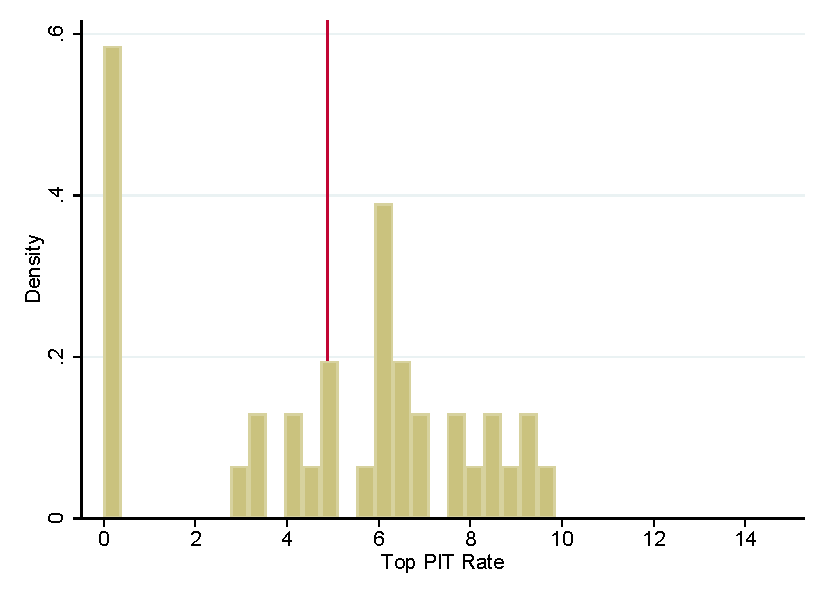
\includegraphics[height=75mm]{../Figures/FigureB1_a.pdf}
				\end{subfigure} &
				\vspace{10pt}

				\begin{subfigure}{0.7\textwidth}
					\caption{2001, Estate Tax States}
					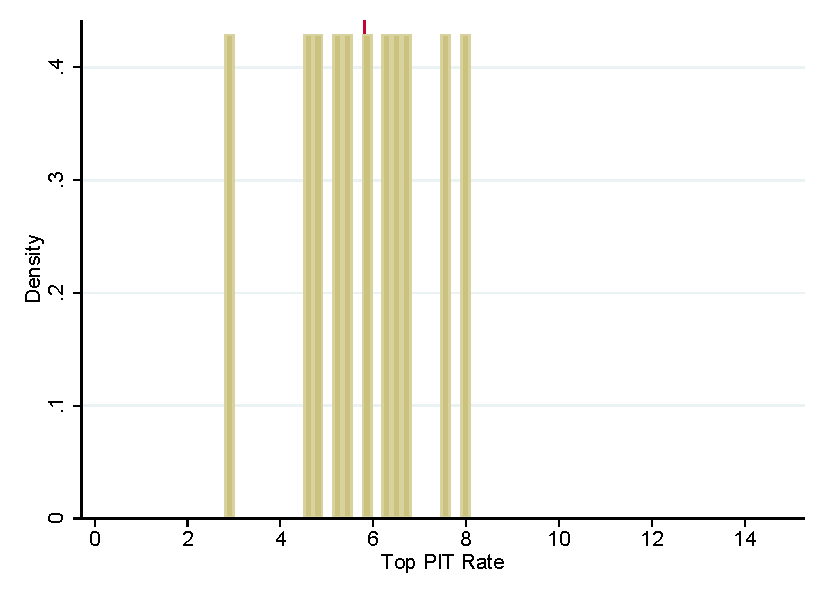
\includegraphics[ height=75mm]{../Figures/FigureB1_b.pdf}
				\end{subfigure} \\
				
				\begin{subfigure}{0.7\textwidth}
					\caption{2017, Non-Estate Tax States}
					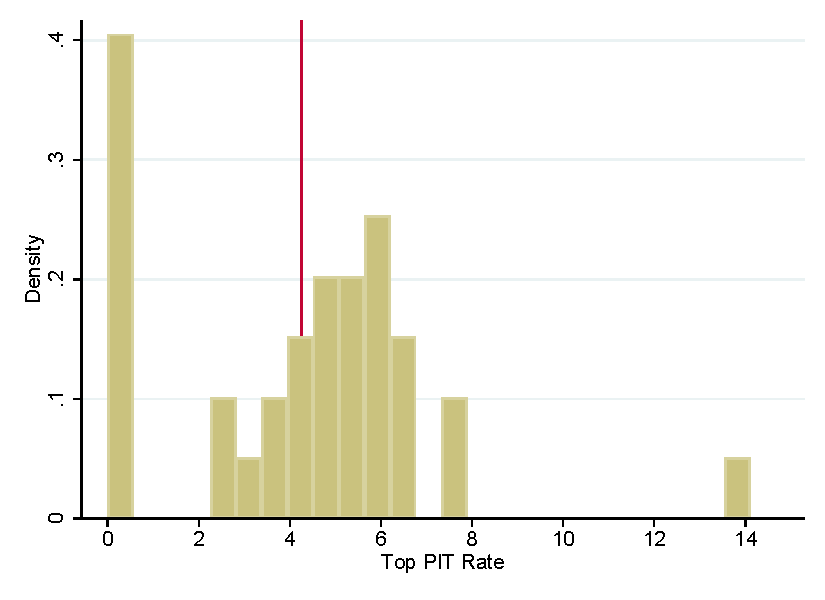
\includegraphics[ height=75mm]{../Figures/FigureB1_c.pdf}
				\end{subfigure} &
				
				\begin{subfigure}{0.7\textwidth}
					\caption{2017, Estate Tax States}
					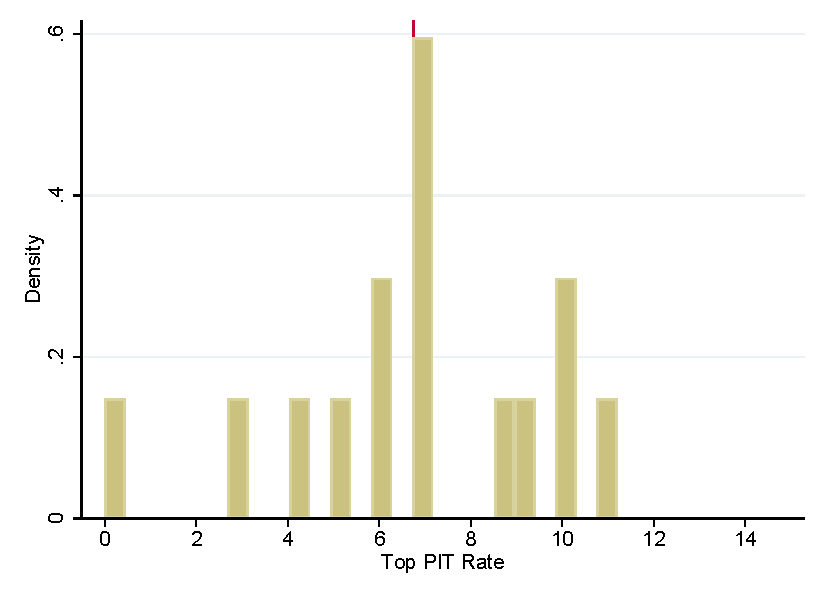
\includegraphics[height=75mm]{../Figures/FigureB1_d.pdf}
				\end{subfigure} \\	
			\end{tabular}
		\end{center}	
{Note: red lines indicate means.}
\end{figure}
\end{landscape}
\clearpage






\begin{figure}
	\centering
	\caption{Average Wealth of Forbes 400 Sample (1982 to 2017)}
	\label{fig:avg_wealth_tsgraph}
	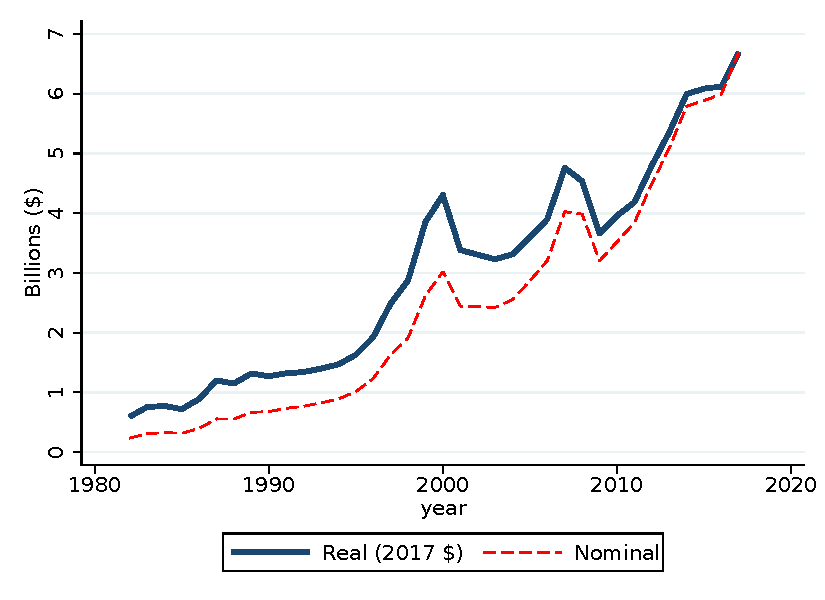
\includegraphics[width=1\textwidth]{../Figures/FigureB2.pdf}
	\caption*{\footnotesize *Based on our sample of Forbes 400 individual-year observations, which excludes those with no data on age or state of residence.}
\end{figure}
\clearpage




\begin{figure}
\centering
\caption{Robustness to Dropping Individual ET States}
\label{newtab33}
	\caption*{Panel A. Difference-in-Difference}
	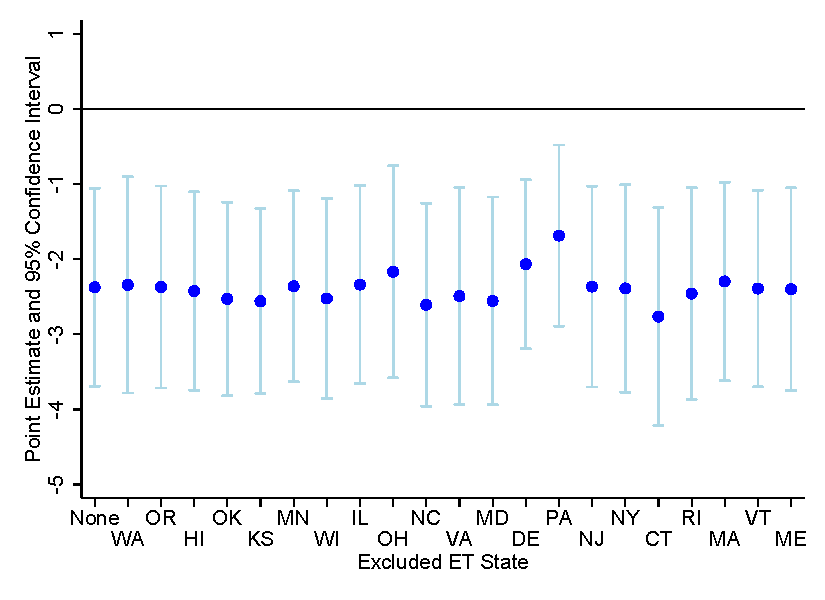
\includegraphics[width=.7\textwidth]{../Figures/FigureB3_a.pdf}
	\caption*{Panel B. Triple-Difference}
	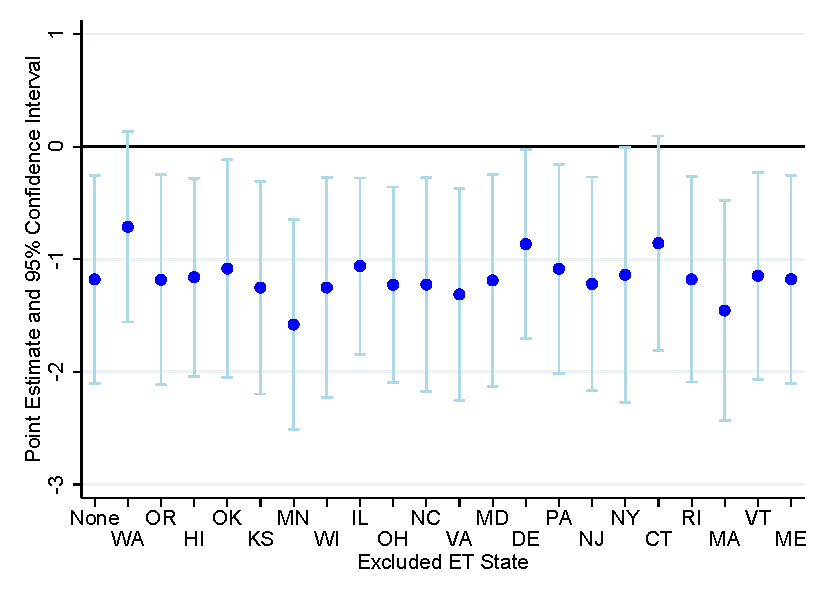
\includegraphics[width=.7\textwidth]{../Figures/FigureB3_b.pdf}
	\caption*{\footnotesize Notes: Panel A shows the estimated coefficient on EIxPost, and its 95\% confidence interval, from the difference-in-difference specification discussed in Section 5.1 dropping, one by one, each state that had an estate tax at some point after 2001. The leftmost coefficient, labeled ``None'', corresponds the baseline estimate shown in Table 2. Point B shows the estimated coefficient on EIxPostxOld, and its 95\% confidence interval, from the triple-difference specification discussed in Section 5.2 dropping, one by one, each state that had an estate tax at some point after 2001. The leftmost coefficient, labeled ``None'', corresponds the baseline estimate shown in Table 3.}
\end{figure}


\begin{figure}
\centering
\caption{Probability of living in High Income Tax State By Age}
	\caption*{Panel A. 1982-2001}
	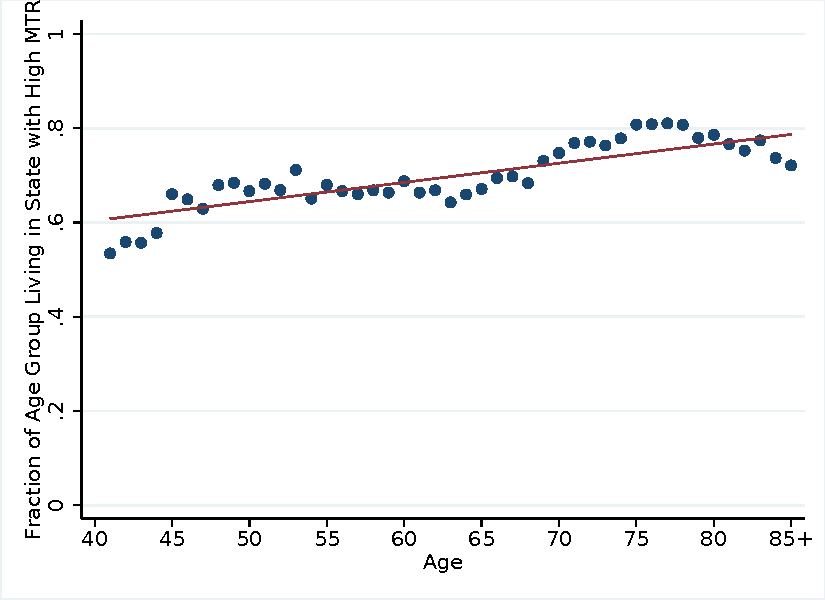
\includegraphics[width=.75\textwidth]{../Figures/FigureB4_a.pdf}
	\caption*{Panel B. 2005-2017}
	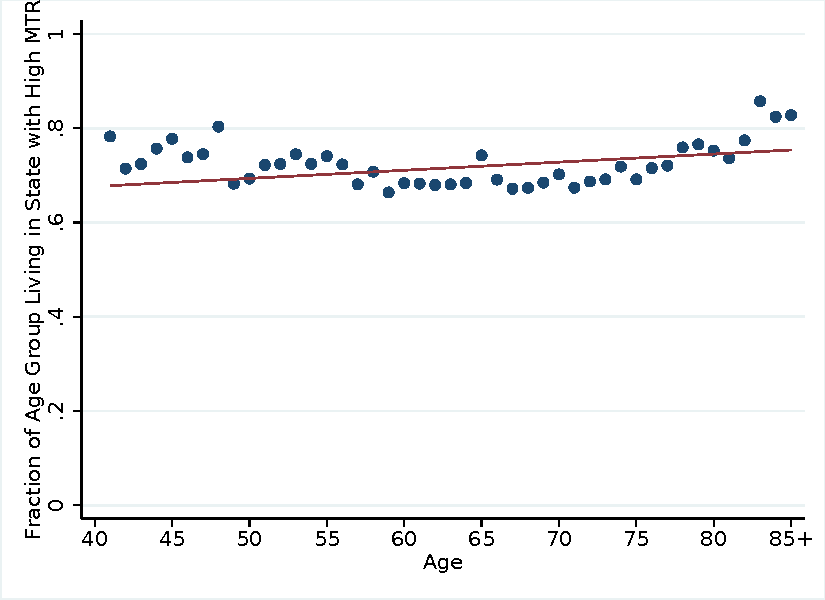
\includegraphics[width=.75\textwidth]{../Figures/FigureB4_b.pdf}
	\caption*{\footnotesize Notes: Age Groups below 40 are excluded. Individuals above 95 are pooled and displayed at Age 96.}
\label{fig:figa1}
\end{figure}
\clearpage



\begin{figure}
\centering
\caption{Number of Federal Estate Taxpayers by State, 2017}
\label{new8map}
	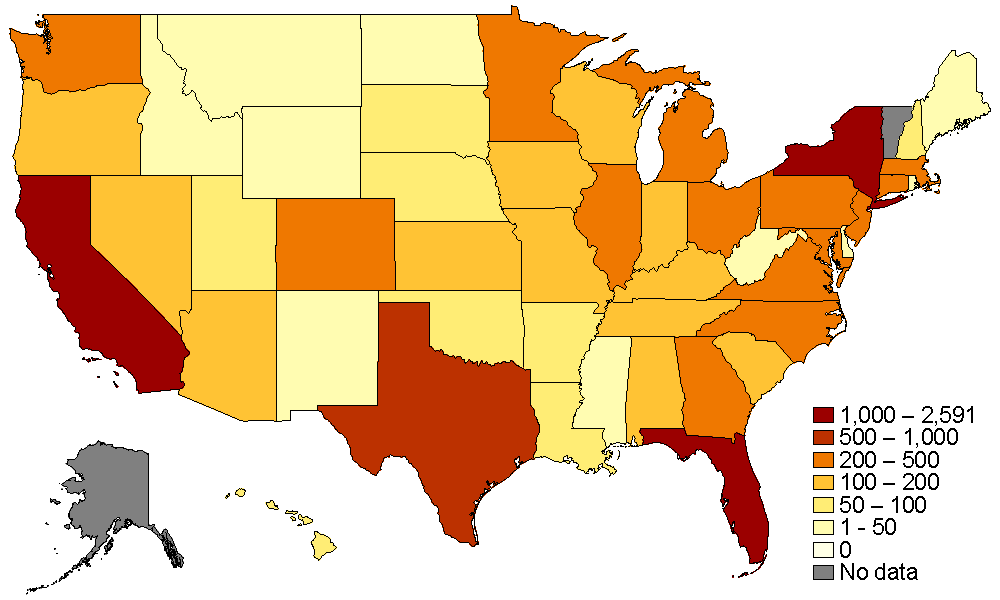
\includegraphics[width=.99\textwidth]{../Figures/FigureB5.pdf}
	\caption*{\footnotesize Source: IRS Statistics on Income.}
\end{figure}
\clearpage



%%%%%%%%%%%%%%%%%%%%%%%%%%%%% NEW MATERIAL TO BE POTENTIAL ADDED TO THE DRAFT %%%%%%%%%%%%%%%%%%%%%%%%%%%%%%%%%%%%%%%%
\if0

\setcounter {table} {0}
\setcounter {figure} {0}
\renewcommand{\thetable}{C\arabic{table}}
\renewcommand{\thefigure}{C\arabic{figure}}



\begin{figure}
\centering
\caption{Forbes 400 Age Distribution, 1982-2017}
	\includegraphics[width=.99\textwidth]{../tables/hist_age.pdf}
\end{figure}


\begin{landscape}
\begin{table}
	\caption{Triple-Difference\\Dependent Variable: Population of Forbes 400}
	\caption*{``Old'' = 60+}
	\centering
	\scalebox{0.65} {
		\renewenvironment{table}[1][]{\ignorespaces}{\unskip}
		\input{../archive/stock_EI_old2001with060.tex}
	}
\end{table}
\clearpage

\begin{table}
	\caption{Triple-Difference\\Dependent Variable: Population of Forbes 400}
	\caption*{``Old'' = 70+ (65-69 year-olds dropped)}
	\centering
	\scalebox{0.65} {
		\renewenvironment{table}[1][]{\ignorespaces}{\unskip}
		\input{../archive/stock_EI_old2001with070.tex}
	}
\end{table}
\clearpage

\begin{table}
	\caption{Triple-Difference\\Dependent Variable: Population of Forbes 400}
	\caption*{``Old'' = 75+ (65-74 year-olds dropped)}
	\centering
	\scalebox{0.65} {
		\renewenvironment{table}[1][]{\ignorespaces}{\unskip}
		\input{../archive/stock_EI_old2001with075.tex}
	}
\end{table}
\clearpage
\end{landscape}

\fi


\end{document}





%%%%%%%%%%%%%%%%%%%%%%%%%%%%%%%%%%%%%%%%%%%%%%%%%%%%%%%%%%%%%%%
%%%%%%%%%%%%%%%%%%%%%%%%%%%%%%%%%%%%%%%%%%%%%%%%%%%%%%%%%%%%%%%
%%%%%%%%%%%%%%%%%%%%%%%%%%%%%%%%%%%%%%%%%%%%%%%%%%%%%%%%%%%%%%%
%%%%%%%%%%%%%%%%%%%%%%%%%%%%%%%%%%%%%%%%%%%%%%%%%%%%%%%%%%%%%%%
\begin{landscape}
\begin{table}
	\centering
	\caption{Probability of Moving Away from ET States and to Non-ET States}
	\caption*{Panel A: All Forbes 400 Individuals Observed in 2001}
	\scalebox{0.9} {
		\renewenvironment{table}[1][]{\ignorespaces}{\unskip}
		\input{../archive/mover_table1.tex}
		\unskip
	}
	\vspace{10pt}
	\caption*{Panel B: Forbes 400 Individuals Observed in 2001 -- 65 and Over}
	\scalebox{0.9} {
		\renewenvironment{table}[1][]{\ignorespaces}{\unskip}
		\input{../archive/mover_table2.tex}
		\unskip
	}
	\vspace{10pt}
	\caption*{Panel C: Forbes 400 Individuals Observed in 2001 -- Under 65}
	\scalebox{0.9} {
		\renewenvironment{table}[1][]{\ignorespaces}{\unskip}
		\input{../archive/mover_table3.tex}
		\unskip
	}
\label{tab:movers_table}
\end{table}

{\footnotesize Notes: ``ET'' denotes status of living in estate tax state; ``Non-ET'' denotes status of living in non-estate tax state. Sample for each column consists of Forbes 400 billionaires observed in both 2001 and year \textit{t}. Second row of each panel shows the percentage of individuals observed in 2001 who, by year \textit{t}, have physical moved from an ET state to a non-ET state. Third row of each panel shows the percentage of individuals observed in 2001 who, by year \textit{t}, have physical moved from a non-ET state to an ET state. Age is measured in 2001.}
\end{landscape}

\clearpage
